\documentclass[10pt]{article}

% Pacotes extras necessários
\usepackage{amsmath}
\usepackage[lmargin=0.5in, rmargin=0.5in, tmargin=0.5in, bmargin=0.5in, includehead, includefoot]{geometry}
\usepackage{amsfonts}
\usepackage[utf8]{inputenc}
\usepackage[portuguese]{babel}
\usepackage{graphicx}
\usepackage{fancyhdr}
\usepackage{setspace}
\usepackage{listings}
\usepackage{url}
\usepackage{enumitem}
\usepackage{appendix} % For creating appendix sections
\usepackage{subcaption} % Use subcaption para legendas modernas

% More defined colors
\usepackage[dvipsnames]{xcolor}

% Define a custom style for the code listing
\lstdefinestyle{mystyle}{
    language=Matlab,
    inputencoding=latin1,
    extendedchars=true,
    backgroundcolor=\color{white},   % Choose the background color
    basicstyle=\ttfamily\footnotesize, % Set the font and size for the code
    numbers=left,                    % Line numbers on the left
    numberstyle=\tiny\color{gray},   % Line numbers style
    numbersep=5pt,                   % Distance of line numbers from the code
    tabsize=2,                       % Set tab size (default is 8 spaces)
    breaklines=true,                 % Automatically wrap long lines
    keywordstyle=\color{blue},       % Keywords in blue
    commentstyle=\color{green!60!black}, % Comments in green
    stringstyle=\color{orange},      % Strings in orange
    frame=single,                    % Draw a frame around the code
    keepspaces=true,                 % Preserve spaces in text
    showspaces=false,                % Don't show spaces in strings
    showstringspaces=false,          % Don't show spaces in strings
    showtabs=false,                  % Don't show tabs in strings
    % Add any other options you need
}

\lstset{style=mystyle} % Set the custom style
 
% Required package
\usepackage{tikz}
\usetikzlibrary{positioning}

\graphicspath{ {./images/} }

% Sets para outras partes
\setlength{\parindent}{1cm}
\setstretch{1.5}
\DeclareMathOperator{\sen}{sen}
\DeclareMathOperator{\sinc}{sinc}

%% Facilidades
%% -- Laplace
\newcommand{\Lap}[1]{\mathcal{L}\left\{#1\right\}}

%% -- Negrito em matemáticas
\newcommand{\bm}[1]{\boldsymbol{#1}}


% ------- Estilo do trabalho -------- %
\fancypagestyle{capa}{
    \fancyhf{}
    \renewcommand\headrulewidth{0pt}
}

\pagestyle{fancy}
\fancyhead{}
\fancyhead[L]{\thepage}
\fancyfoot{}
% ----------------------------------- %

% Dados do Grupo
\title{ Robótica e Automação - Trabalho Nº3}
\author{
    Leonardo Soares da Costa Tanaka - DRE: 121067652 \\
    Engenharia de Controle e Automação/UFRJ \\
    Rio de Janeiro, Brasil \\
    Dezembro de 2024
}
\date{}

\begin{document}
\maketitle
\thispagestyle{capa}

\section{Introdução}

Para a resolução do trabalho, foi usado o manipulador Kinova Gen3 Ultra lightweight (www.kinovarobotics.com) da Kinova
Inc.. A estrutura cinemática deste manipulador de 7 juntas pode ser vista na figura a seguir:

\begin{figure}[h]
    \centering
    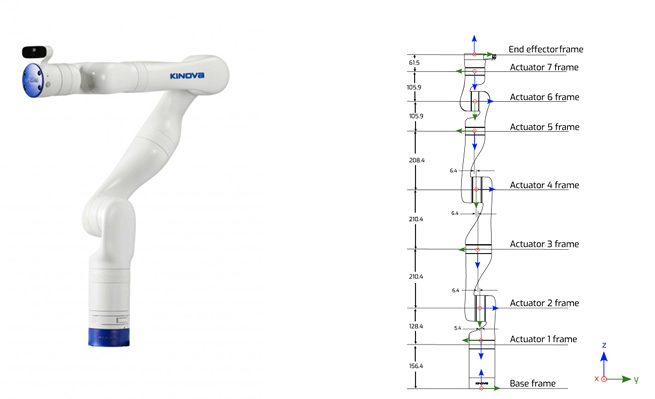
\includegraphics[scale=1]{kinova.png}
    \caption{Foto e Diagrama do manipulador Kinova}
\end{figure}

Além disso, os parâmetros de Denavit-Hartenberg do manipulador são apresentados na Tabela~\ref{tab:dh_parameters}.
Foi considerado que a orientação do sistema de coordenadas 0 com relação à base é dado por
$R_{b0}=R_x(\pi)$ onde $R_x(\cdot)$ é uma rotação elementar ao redor do eixo x.

\begin{table}[h!]
    \centering
    \begin{tabular}{|c|c|c|c|c|c|}
    \hline
    \textbf{Junta} & $\alpha$ (rad) & $A$ (m) & $\theta$ (rad) & $D$ (m) & \textbf{Offset (rad)} \\ \hline
    1 & $\pi/2$ & 0 & $\theta_1$ & $-0.2848$ & $\pi$ \\ \hline
    2 & $\pi/2$ & 0 & $\theta_2$ & $-0.0118$ & $\pi$ \\ \hline
    3 & $\pi/2$ & 0 & $\theta_3$ & $-0.4208$ & $\pi$ \\ \hline
    4 & $\pi/2$ & 0 & $\theta_4$ & $-0.0128$ & $\pi$ \\ \hline
    5 & $\pi/2$ & 0 & $\theta_5$ & $-0.3143$ & $\pi$ \\ \hline
    6 & $\pi/2$ & 0 & $\theta_6$ & 0 & $\pi$ \\ \hline
    7 & $\pi$ & 0 & $\theta_7$ & 0 & $\pi$ \\ \hline
    \end{tabular}
    \caption{Parâmetros de Denavit-Hartenberg Standard do Kinova Gen3}
    \label{tab:dh_parameters}
\end{table}

Ademais, os parâmetros dinâmicos deste sistema robótico são dados no arquivo urdf, kinova\_gen3.urdf,
onde podem ser obtidos os parâmetros da massa, centro de massa e momento de inércia
de cada elo no formato urdf. Podendo ser estruturados nas Tabelas~\ref{tab:joints} e~\ref{tab:links}:

\begin{table}[h!]
    \centering
    \begin{tabular}{|c|c|c|c|c|c|c|}
    \hline
    \textbf{Joint i} & \textbf{Parent} & \textbf{Child} & \textbf{xyz} & \textbf{rpy} & \textbf{Type} & \textbf{Axis} \\ \hline
    1 & base\_link & shoulder\_link & 0, 0, 0.15643 & 3.1416, 0, 0 & continuous & 0, 0, 1 \\ \hline
    2 & shoulder\_link & half\_arm\_1\_link & 0, 0.005375, -0.12838 & 1.5708, 0, 0 & revolute & 0, 0, 1 \\ \hline
    3 & half\_arm\_1\_link & half\_arm\_2\_link & 0, -0.21038, -0.006375 & -1.5708, 0, 0 & continuous & 0, 0, 1 \\ \hline
    4 & half\_arm\_2\_link & forearm\_link & 0, 0.006375, -0.21038 & 1.5708, 0, 0 & revolute & 0, 0, 1 \\ \hline
    5 & forearm\_link & spherical\_wrist\_1\_link & 0, -0.20843, -0.006375 & -1.5708, 0, 0 & continuous & 0, 0, 1 \\ \hline
    6 & spherical\_wrist\_1\_link & spherical\_wrist\_2\_link & 0, 0.00017505, -0.10593 & 1.5708, 0, 0 & revolute & 0, 0, 1 \\ \hline
    7 & spherical\_wrist\_2\_link & bracelet\_link & 0, -0.10593, -0.00017505 & -1.5708, 0, 0 & continuous & 0, 0, 1 \\ \hline
    8 & bracelet\_link & end\_effector\_link & 0, 0, -0.061525 & 3.14159, 0, 0 & fixed & 0, 0, 0 \\ \hline
    \end{tabular}
    \caption{URDF das juntas do manipulador Kinova}
    \label{tab:joints}
\end{table}
\begin{table}[h!]
    \centering
    \begin{tabular}{|c|c|c|c|}
    \hline
    \textbf{Link}          & \textbf{Origem (xyz)}   & \textbf{Massa(kg)} & \textbf{Inércia (ixx iyy izz ixy ixz iyz)} \\ \hline
    base\_link             & -0.000648 -0.000166 0.084487 & 1.697               & 0.004622 0.004495 0.002079 9E-06 6E-05 9E-06 \\ \hline
    shoulder\_link         & -2.3E-05 -0.010364 -0.07336  & 1.377               & 0.00457 0.004831 0.001409 1E-06 2E-06 0.000448 \\ \hline
    half\_arm\_1\_link     & -4.4E-05 -0.09958 -0.013278  & 1.163               & 0.011088 0.001072 0.011255 5E-06 0 -0.000691 \\ \hline
    half\_arm\_2\_link     & -4.4E-05 -0.006641 -0.117892 & 1.163               & 0.010932 0.011127 0.001043 0 -7E-06 0.000606 \\ \hline
    forearm\_link          & -1.8E-05 -0.075478 -0.015006 & 0.93                & 0.008147 0.000631 0.008316 -1E-06 0 -0.0005 \\ \hline
    spherical\_wrist\_1\_link & 1E-06 -0.009432 -0.063883  & 0.678               & 0.001596 0.001607 0.000399 0 0 0.000256 \\ \hline
    spherical\_wrist\_2\_link & 1E-06 -0.045483 -0.00965   & 0.678               & 0.001641 0.00041 0.001641 0 0 -0.000278 \\ \hline
    bracelet\_link         & -9.3E-05 0.000132 -0.022905  & 0.364               & 0.000214 0.000223 0.00024 0 1E-06 -2E-06 \\ \hline
    end\_effector\_link    & 0 0 0                     & 0                   & 0 0 0 0 0 0 \\ \hline
    \end{tabular}
    \caption{URDF dos elos do manipulador Kinova com rpy="0 0 0" para todos os elos}
    \label{tab:links}
\end{table}
Para saber a representação dos centros de massa nos sistemas de coordenadas do Denavit-Hartenberg que será usado para gerar o SerialLink,
é necessário  obter as transformações homogêneas entre os sistemas de coordenadas das duas representações a partir do Denavit-Hartenberg e do URDF.
A seguir temos as transformações homogêneas:

\begin{equation}
T_1 = \begin{bmatrix} 
1 & 0 & 0 & 0 \\ 
0 & 0 & 1 & 0.12837 \\ 
0 & -1 & 0 & 0 \\ 
0 & 0 & 0 & 1 
\end{bmatrix}, \quad
T_2 = \begin{bmatrix} 
-1 & 0 & 0 & 0 \\ 
0 & 0 & 1 & 0.006425 \\ 
0 & 1 & 0 & -0.00001 \\ 
0 & 0 & 0 & 1 
\end{bmatrix}, \quad
T_3 = \begin{bmatrix} 
1 & 0 & 0 & 0 \\ 
0 & 0 & 1 & 0.21041 \\ 
0 & -1 & 0 & 0.00005 \\ 
0 & 0 & 0 & 1 
\end{bmatrix}, 
\end{equation}

\begin{equation}
T_4 = \begin{bmatrix} 
-1 & 0 & 0 & 0 \\ 
0 & 0 & 1 & 0.006475 \\ 
0 & 1 & 0 & 0.00003 \\ 
0 & 0 & 0 & 1 
\end{bmatrix}, \quad
T_5 = \begin{bmatrix} 
1 & 0 & 0 & 0 \\ 
0 & 0 & 1 & 0.1059 \\ 
0 & -1 & 0 & 0.0001 \\ 
0 & 0 & 0 & 1 
\end{bmatrix}, \quad
T_6 = \begin{bmatrix} 
-1 & 0 & 0 & 0 \\ 
0 & 0 & 1 & -0.00007505 \\ 
0 & 1 & 0 & -0.00003 \\ 
0 & 0 & 0 & 1 
\end{bmatrix},
\end{equation}

\begin{equation}
T_7 = \begin{bmatrix} 
1 & 0 & 0 & 0 \\ 
0 & -1 & 0 & -0.0002501 \\ 
0 & 0 & -1 & 0.10596 \\ 
0 & 0 & 0 & 1 
\end{bmatrix}.
\end{equation}

Os parâmetros dinâmicos do robô incluem massa ($L(i).m$), centro de massa ($L(i).r$) e momentos de inércia ($L(i).I$) para cada elo.
A massa de cada elo é especificada diretamente, enquanto o centro de massa é calculado utilizando as transformações homogêneas $T_i$ aplicadas às coordenadas locais do elo, resultando em $\text{cmass}_i = T_i \cdot [x \; y \; z \; 1]^T$, com $L(i).r$ sendo os três primeiros elementos.
Os momentos de inércia são definidos como um vetor contendo os valores em relação aos eixos principais e os produtos de inércia, usados na modelagem dinâmica.
Além disso, a inércia dos motores é inicializada como $L(i).Jm = 0$ para todos os elos.

Para este manipulador, foi projetado os seguintes controladores:

\begin{enumerate}
    \item \textbf{Controlador PD:}
    \begin{equation}
        \tau = K_p (\theta_d - \theta) + K_d (\dot{\theta}_d - \dot{\theta}),
    \end{equation}
    de forma que os polos dominantes de cada elo tenham frequência natural \(\omega_n = 10 \, \text{rad/s}\) e coeficiente de amortecimento \(\zeta = 1\).

    \item \textbf{Controlador P-PI:}
    \begin{equation}
        \tau = K_d e_2 + K_i \int e_2 \, dt + K_a \ddot{\theta}_d,
        \label{eq:pi_ppi}
    \end{equation}
    onde
    \begin{equation}
        e_2 = K_p (\theta_d - \theta) + (\dot{\theta}_d - \dot{\theta}),
        \label{eq:p_ppi}
    \end{equation}
    também garantindo \(\omega_n = 10 \, \text{rad/s}\) e \(\zeta = 1\).

    \item \textbf{Controlador por Torque Computado + PD:}
    \begin{equation}
        \tau = M(\theta) u + C(\theta, \dot{\theta}) \dot{\theta} + G(\theta),
    \end{equation}
    com
    \begin{equation}
        u = K_p (\theta_d - \theta) + K_d (\dot{\theta}_d - \dot{\theta}) + \ddot{\theta}_d,
    \end{equation}
    assegurando \(\omega_n = 10 \, \text{rad/s}\) e \(\zeta = 1\).

    \item \textbf{Controlador de Slotine \& Li:}
    \begin{equation}
        \tau = M(\theta) \ddot{\theta}_r + C(\theta, \dot{\theta}) \dot{\theta}_r + G(\theta) - K_d \sigma,
    \end{equation}
    onde
    \begin{equation}
        \sigma = (\dot{\theta} - \dot{\theta}_d) + \Lambda (\theta - \theta_d) = \dot{\theta} - \dot{\theta}_r,
    \end{equation}
    garantindo desempenho similar aos itens anteriores.
\end{enumerate}

A trajetória desejada, em radianos, é dada por:
\begin{align}
    \theta_{1d} &= 0.5236 \cos(\omega_n t), \\
    \theta_{2d} &= 0.2618 + 0.2618 \cos(\omega_n t), \\
    \theta_{3d} &= \pi, \\
    \theta_{4d} &= -2.2689 + 0.2618 \cos(1.2 \omega_n t), \\
    \theta_{5d} &= 0.0, \\
    \theta_{6d} &= 0.9599 + 0.2618 \cos(1.3 \omega_n t), \\
    \theta_{7d} &= \pi/2.
\end{align}

O comportamento do sistema em malha fechada foi simulado para as condições iniciais do manipulador definidas pelos ângulos de juntas \(\theta = [0, 15, 180, -130, 0, 55, 90] \, (\text{graus})\), considerando as seguintes trajetórias desejadas:
\begin{itemize}
    \item Trajetória rápida com \(\omega_n = \pi\);
    \item Trajetória lenta com \(\omega_n = \pi/2\).
\end{itemize}

Adicionalmente, foi analisado o caso em que a massa do último elo (\textit{end-effector link}) muda para \(m_l = 10 \, \text{kg}\).
As simulações irão avaliar a estabilidade e o desempenho de cada controlador projetado sob essa nova condição.
Isso foi seguido conforme a mudança da massa, o deslocamento do centro de massa e a mudança da inércia do último elo que
foram implementados seguindo as seguintes formulações:
\begin{equation}
    m_7 = 10 + 0.364 = 10.364,
\end{equation}
\begin{equation}
    r = \frac{0.364 \cdot \begin{bmatrix} -0.0001 \\ -0.0004 \\ 0.1289 \end{bmatrix} + 10 \cdot \begin{bmatrix} 0 \\ 0 \\ 0.1674 \end{bmatrix}}{10.364}
\end{equation}
\begin{equation}
    I_P = I_c - m \left( \vec{r}_c \vec{r}_c \cdot - ||\vec{r}_c||^2 \, I \right)
\end{equation}

\section{Desenvolvimento}

Esta seção propõe o projeto e análise de quatro estratégias de controle – PD, P-PI, Torque Computado com PD e Slotine \& Li – ajustadas para assegurar pólos dominantes com frequência natural \(\omega_n = 10 \, \text{rad/s}\) e coeficiente de amortecimento \(\zeta = 1\).
As simulações consideram trajetórias rápidas (\(\omega_n = \pi\)) e lentas (\(\omega_n = \pi/2\)), além de mudanças no manipulador, como o aumento da massa do último elo para \(m_{l2} = 10 \, \text{kg}\).
O objetivo é avaliar o desempenho e a estabilidade de cada controlador, destacando suas vantagens e limitações em diferentes cenários operacionais.
O polinômio característico associado aos pólos dominantes desejados é dado por:
\begin{equation}
    p_c(s) = s^2 + 20s + 100
\end{equation}

\subsection{Controlador PD}

Considera-se que \(M(\theta)\) é expressa como:

\begin{equation}
    M(\theta) = \bar{M} + \Delta M(\theta),
\end{equation}
em que \(\bar{M} \in \mathbb{R}^{n \times n}\) é uma matriz positiva, diagonal e constante, i.e.,
\begin{equation}
    \bar{M} = \text{diag}(\bar{m}_1, \cdots, \bar{m}_n) > 0, \quad \bar{m}_i \in \mathbb{R}.
\end{equation}

Para seu cálculo, cada elemento diagonal $\bar{m}_i$ é determinado pela soma dos momentos de inércia ($L(j).I(3,3)$) e das contribuições das massas dos elos ($L(j).m$), ponderadas pela distância do centro de massa ($\|\mathbf{r}_j\|^2$) e a distância acumulada das juntas anteriores até o elo atual. A distância acumulada é calculada como o quadrado do deslocamento das juntas ($|L(j).d|^2$).
Dessa forma, considerando o modelo dinâmico do manipulador, tem-se:
\begin{equation}
    \tau = (\bar{M} + \Delta M(\theta)) \ddot{\theta} + C(\theta,\dot{\theta}) \dot{\theta} + G(\theta)
\end{equation}

Portanto, o modelo dinâmico do manipulador pode ser escrito como:
\begin{equation}
    \tau = \bar{M} \ddot{\theta} + d,
\label{eq:dinamica_simplificada}
\end{equation}
em que: $d = \Delta M(\theta) \ddot{\theta} + C(\theta,\dot{\theta}) \dot{\theta} + G(\theta)$.

Ao utilizar o controlador PD ($u = - K_d \dot{\tilde{\theta}} - K_p \tilde{\theta}$) é obtido o seguinte polinômio característico do manipulador:
\begin{equation}
    p_c(s) = \bar{M}s^2 + K_d s + K_p
\end{equation}
em que $K_d = 20\bar{M}$ e $K_p = 100\bar{M}$  para respeitar as especificações do projeto.
A seguir temos o diagrama do controlador PD com os ganhos projetados implementado no Simulink:

\newpage

\begin{figure}[h]
    \centering
    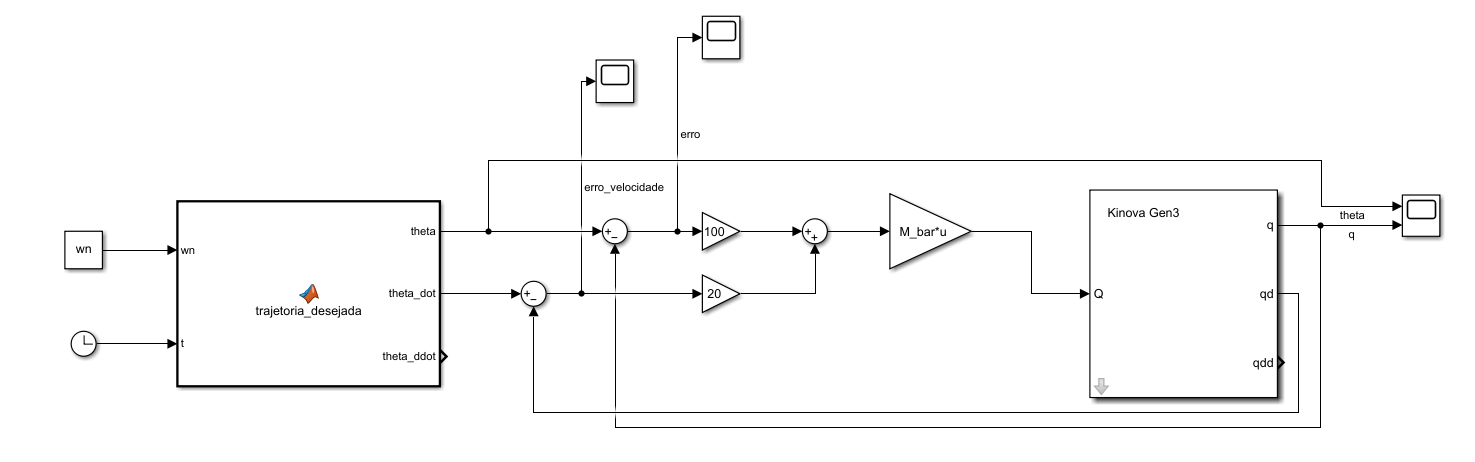
\includegraphics[scale=0.55]{diagrama_pd.png}
    \caption{Diagrama do controlador PD}
\end{figure}

Além disso, foi avaliado esse controlador para um intervalo de 10 segundos com um $\omega_n = \pi$.
Isso foi feito observando as posições das juntas,
o erro entre as posições das juntas e as posições das trajetórias desejadas e
o erro entre as velocidades das juntas e as velocidades das trajetórias desejadas.
A seguir temos os gráficos:

\begin{figure}[h!]
    \centering
    \begin{subfigure}[b]{0.45\textwidth}
        \centering
        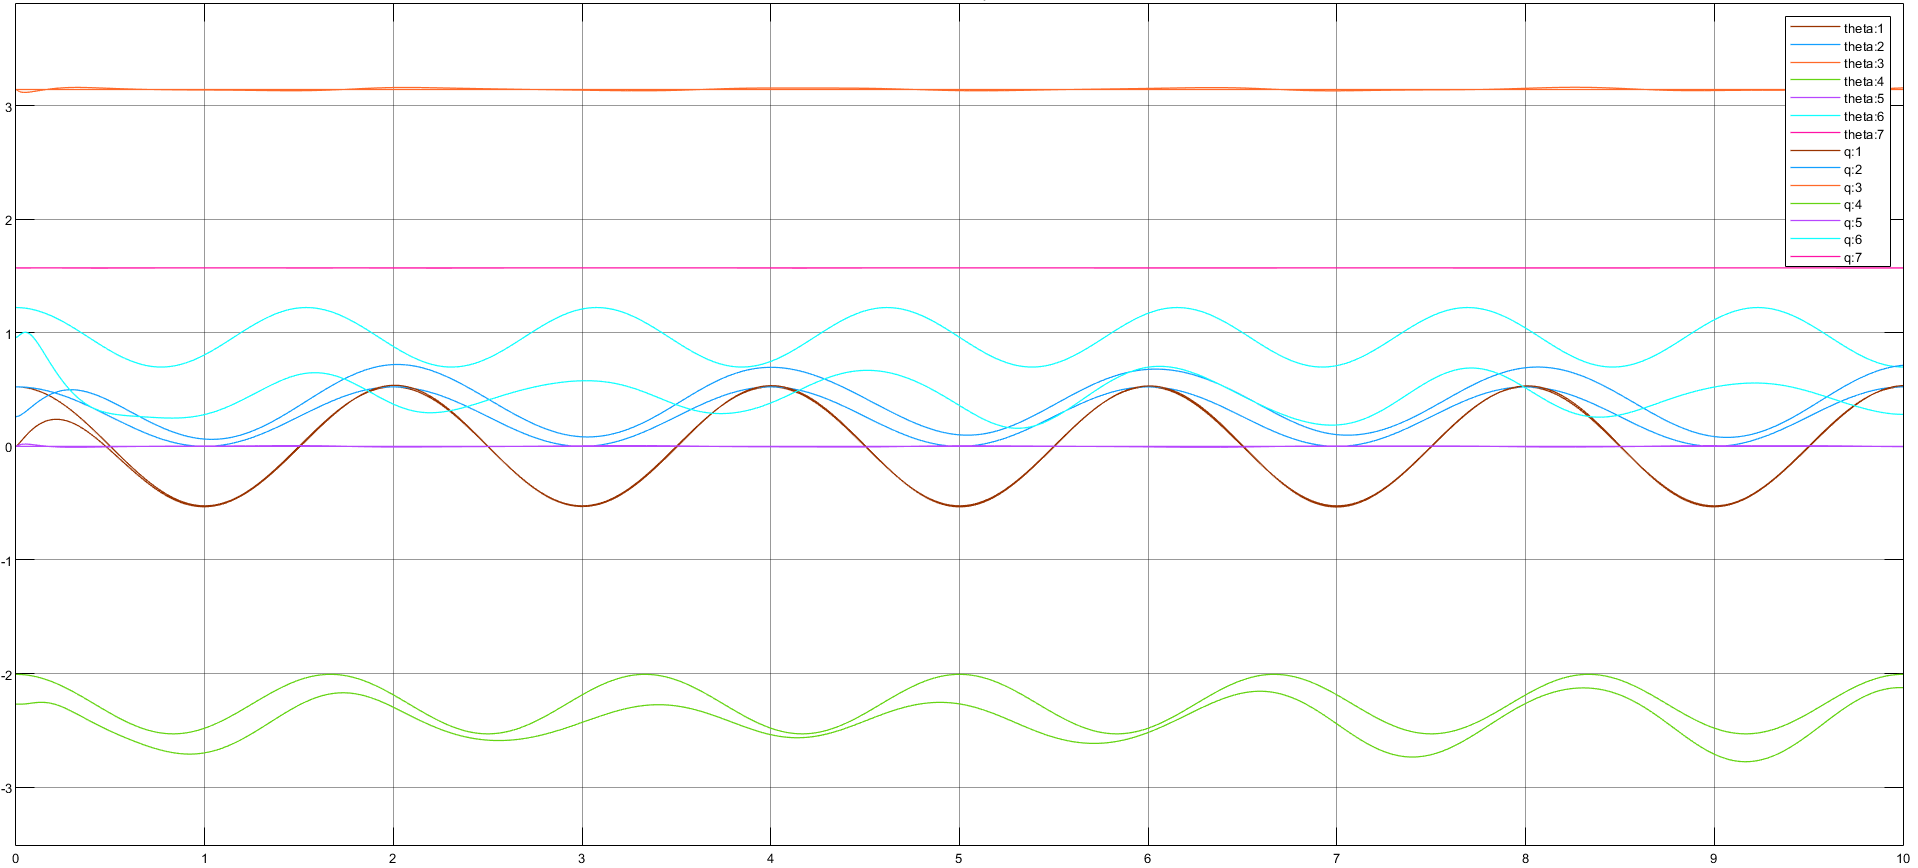
\includegraphics[width=\linewidth]{posicao_pd_pi.png}
        \caption{Posições das juntas}
        \label{fig:posicao_pd_pi}
    \end{subfigure}%
    \hfill
    \begin{subfigure}[b]{0.45\textwidth}
        \centering
        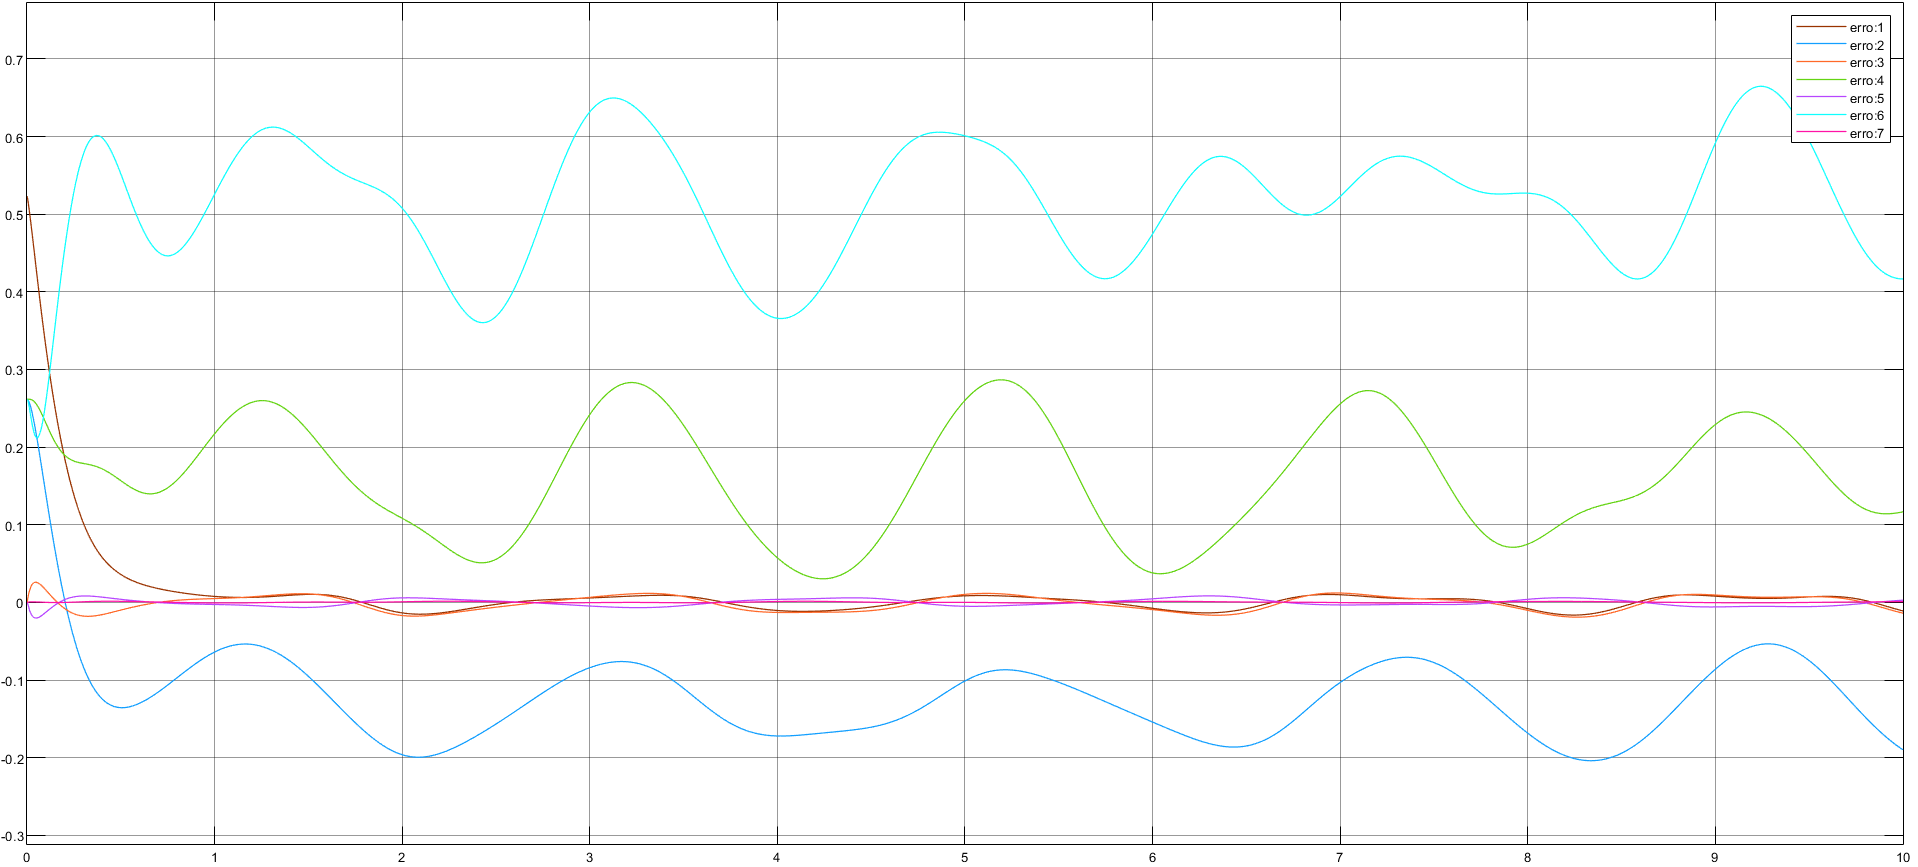
\includegraphics[width=\linewidth]{erro_pd_pi.png}
        \caption{Erros de posições das juntas}
        \label{fig:erro_pd_pi}
    \end{subfigure}%
    \hfill
    \begin{subfigure}[b]{0.45\textwidth}
        \centering
        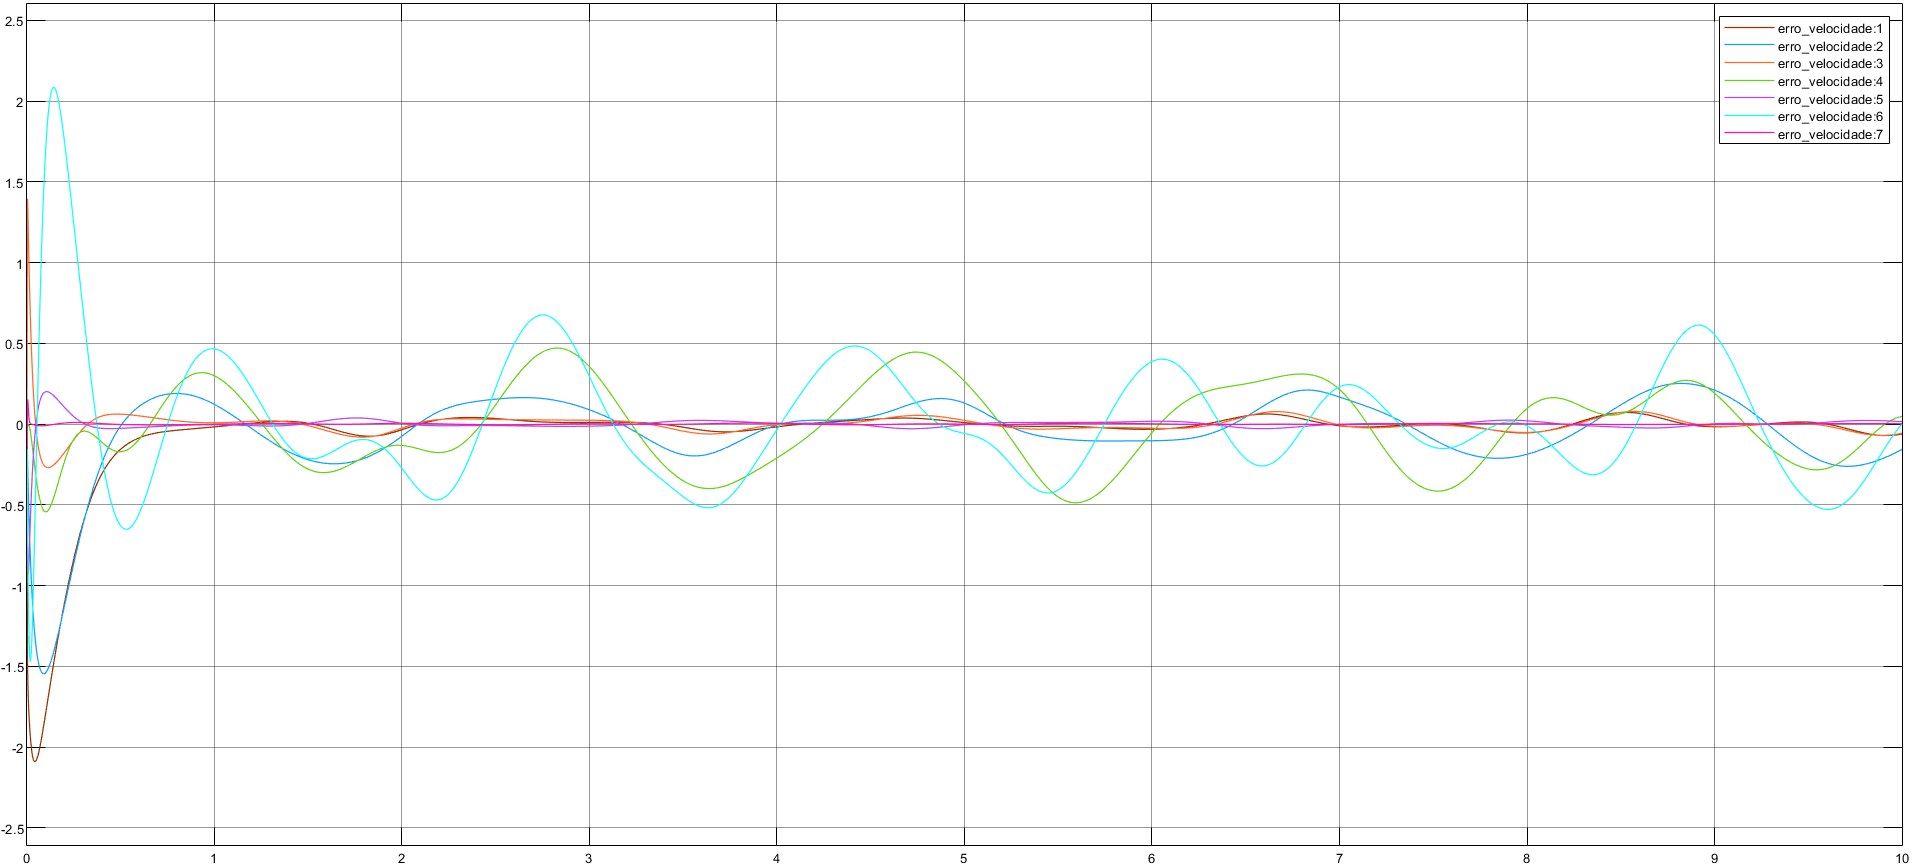
\includegraphics[width=\linewidth]{erro_velocidade_pd_pi.png}
        \caption{Erros de velocidades das juntas}
        \label{fig:erro_velocidade_pd_pi}
    \end{subfigure}%
    \caption{Controlador PD ($\omega_n = \pi$)}
    \label{fig:imagens_pd_pi}
\end{figure}

Isso também foi feito para $\omega_n = \pi/2$. Obtendo os seguintes resultados:

\newpage

\begin{figure}[h!]
    \centering
    \begin{subfigure}[b]{0.45\textwidth}
        \centering
        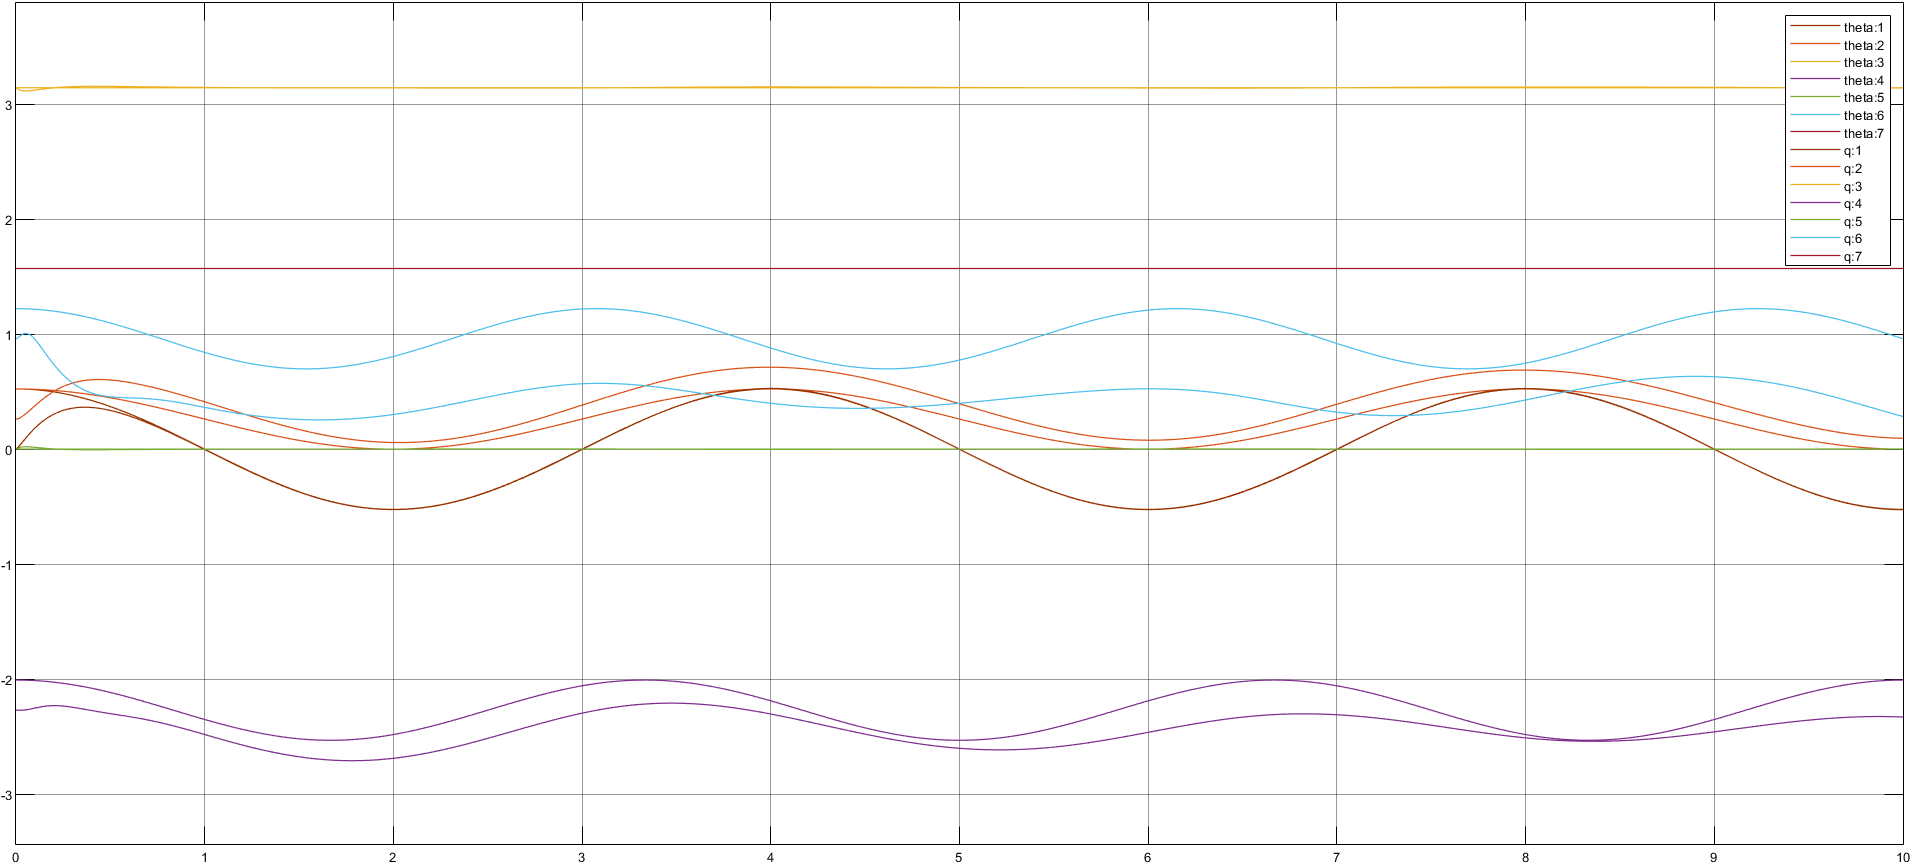
\includegraphics[width=\linewidth]{posicao_pd_pi2.png}
        \caption{Posições das juntas}
        \label{fig:posicao_pd_pi2}
    \end{subfigure}%
    \hfill
    \begin{subfigure}[b]{0.45\textwidth}
        \centering
        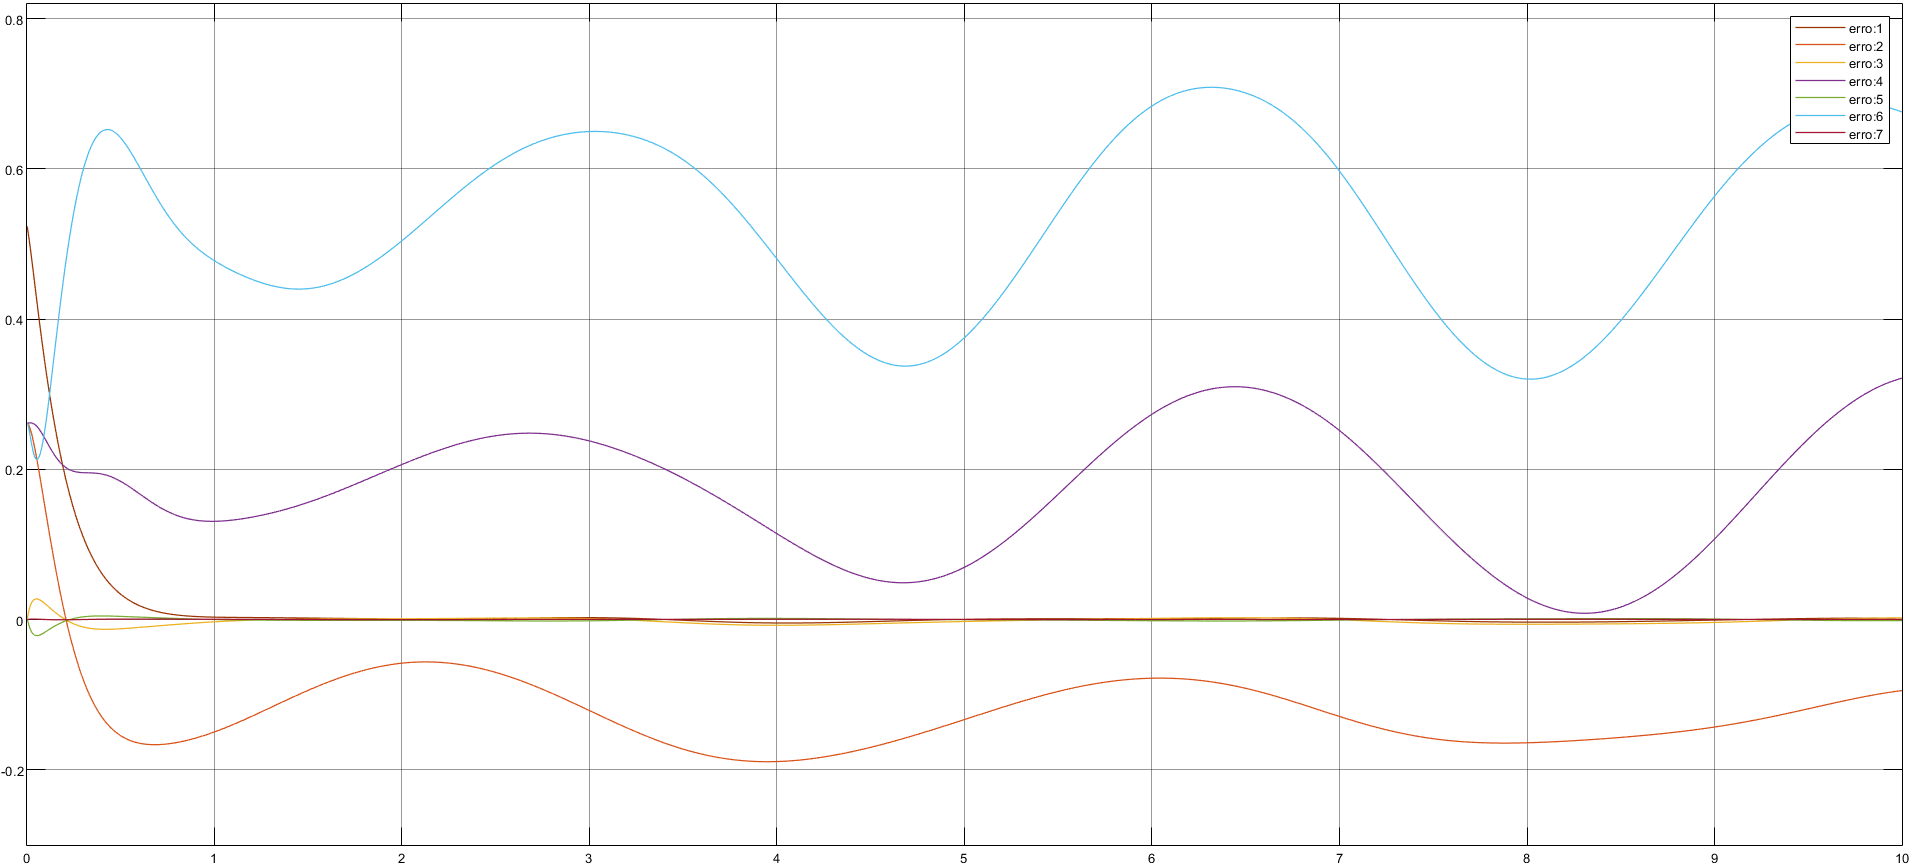
\includegraphics[width=\linewidth]{erro_pd_pi2.png}
        \caption{Erros de posições das juntas}
        \label{fig:erro_pd_pi2}
    \end{subfigure}%
    \hfill
    \begin{subfigure}[b]{0.45\textwidth}
        \centering
        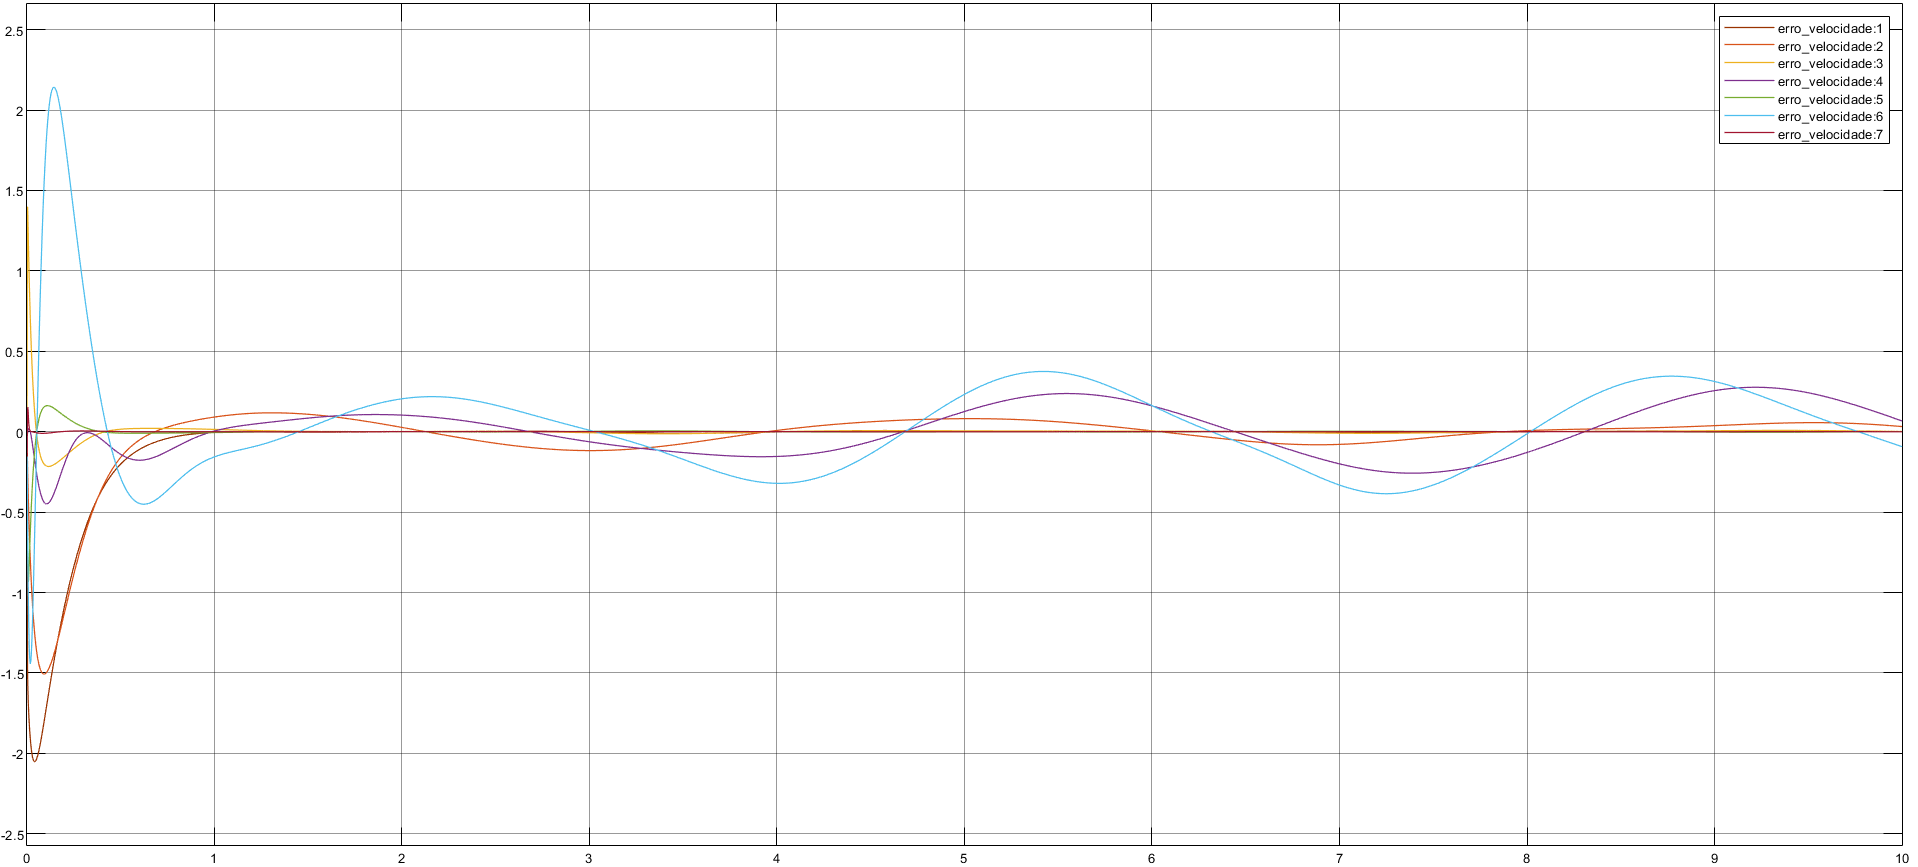
\includegraphics[width=\linewidth]{erro_velocidade_pd_pi2.png}
        \caption{Erros de velocidades das juntas}
        \label{fig:erro_velocidade_pd_pi2}
    \end{subfigure}%
    \caption{Controlador PD ($\omega_n = \pi/2$)}
    \label{fig:imagens_pd_pi2}
\end{figure}

Além disso, foi feito a simulação com a massa adicional de 10kg para $\omega_n = \pi$:

\begin{figure}[h!]
    \centering
    \begin{subfigure}[b]{0.45\textwidth}
        \centering
        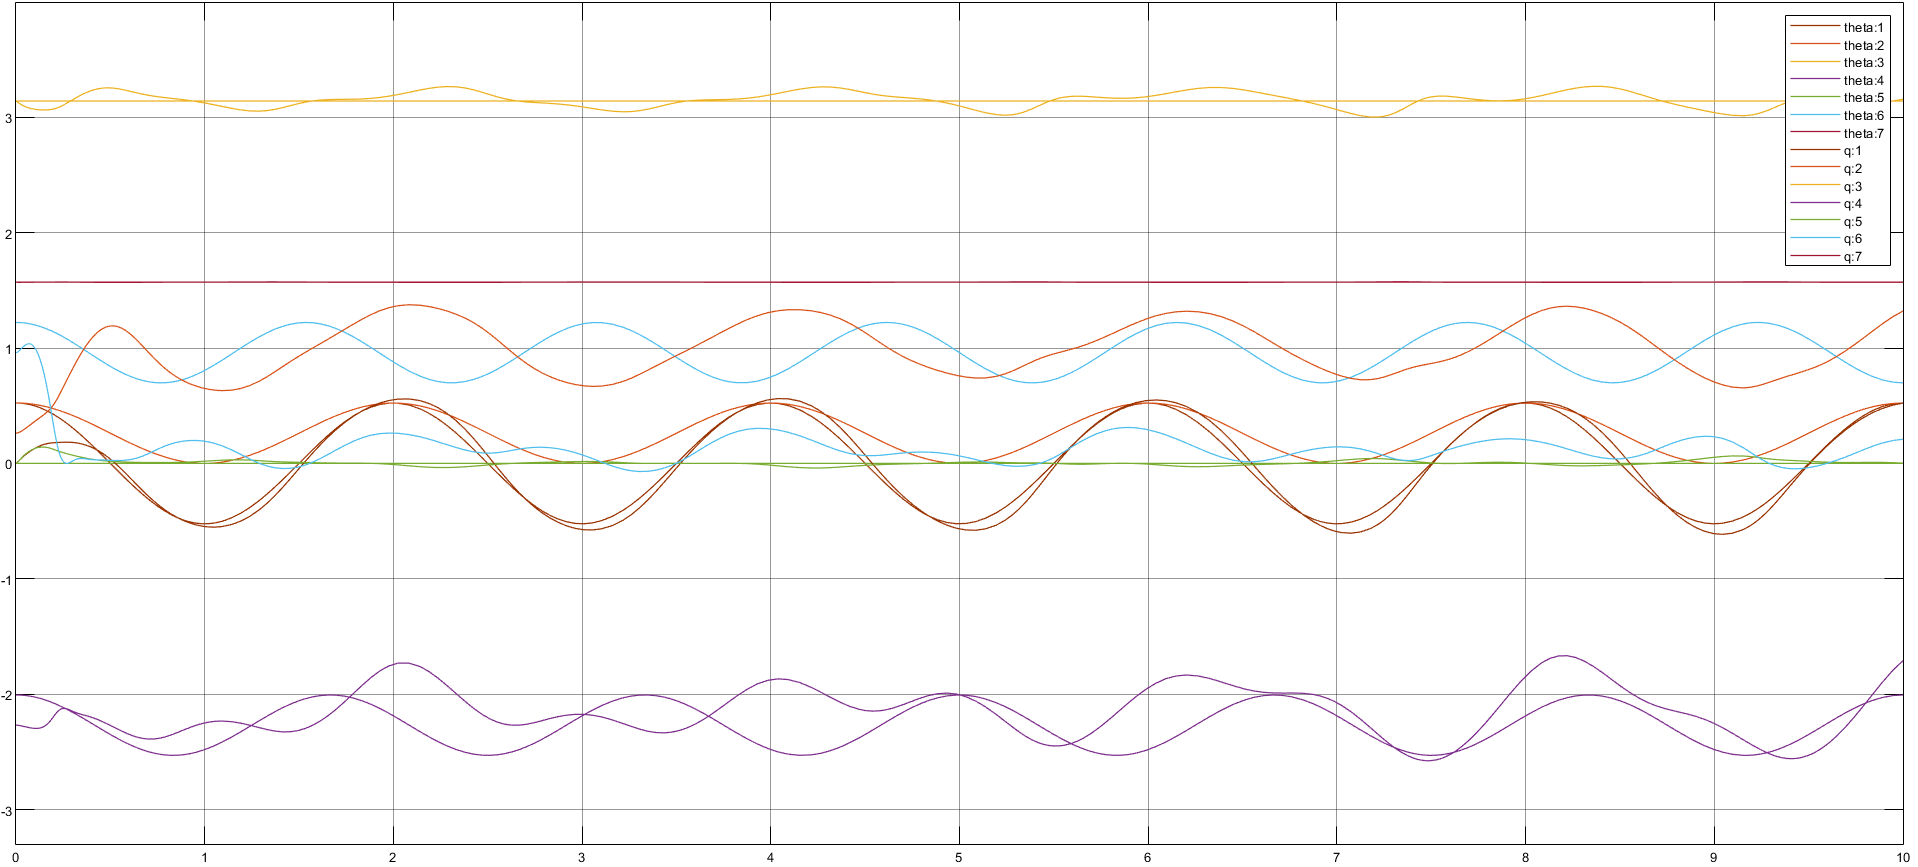
\includegraphics[width=\linewidth]{posicao_pd_pi_m.png}
        \caption{Posições das juntas}
        \label{fig:posicao_pd_pi_m}
    \end{subfigure}%
    \hfill
    \begin{subfigure}[b]{0.45\textwidth}
        \centering
        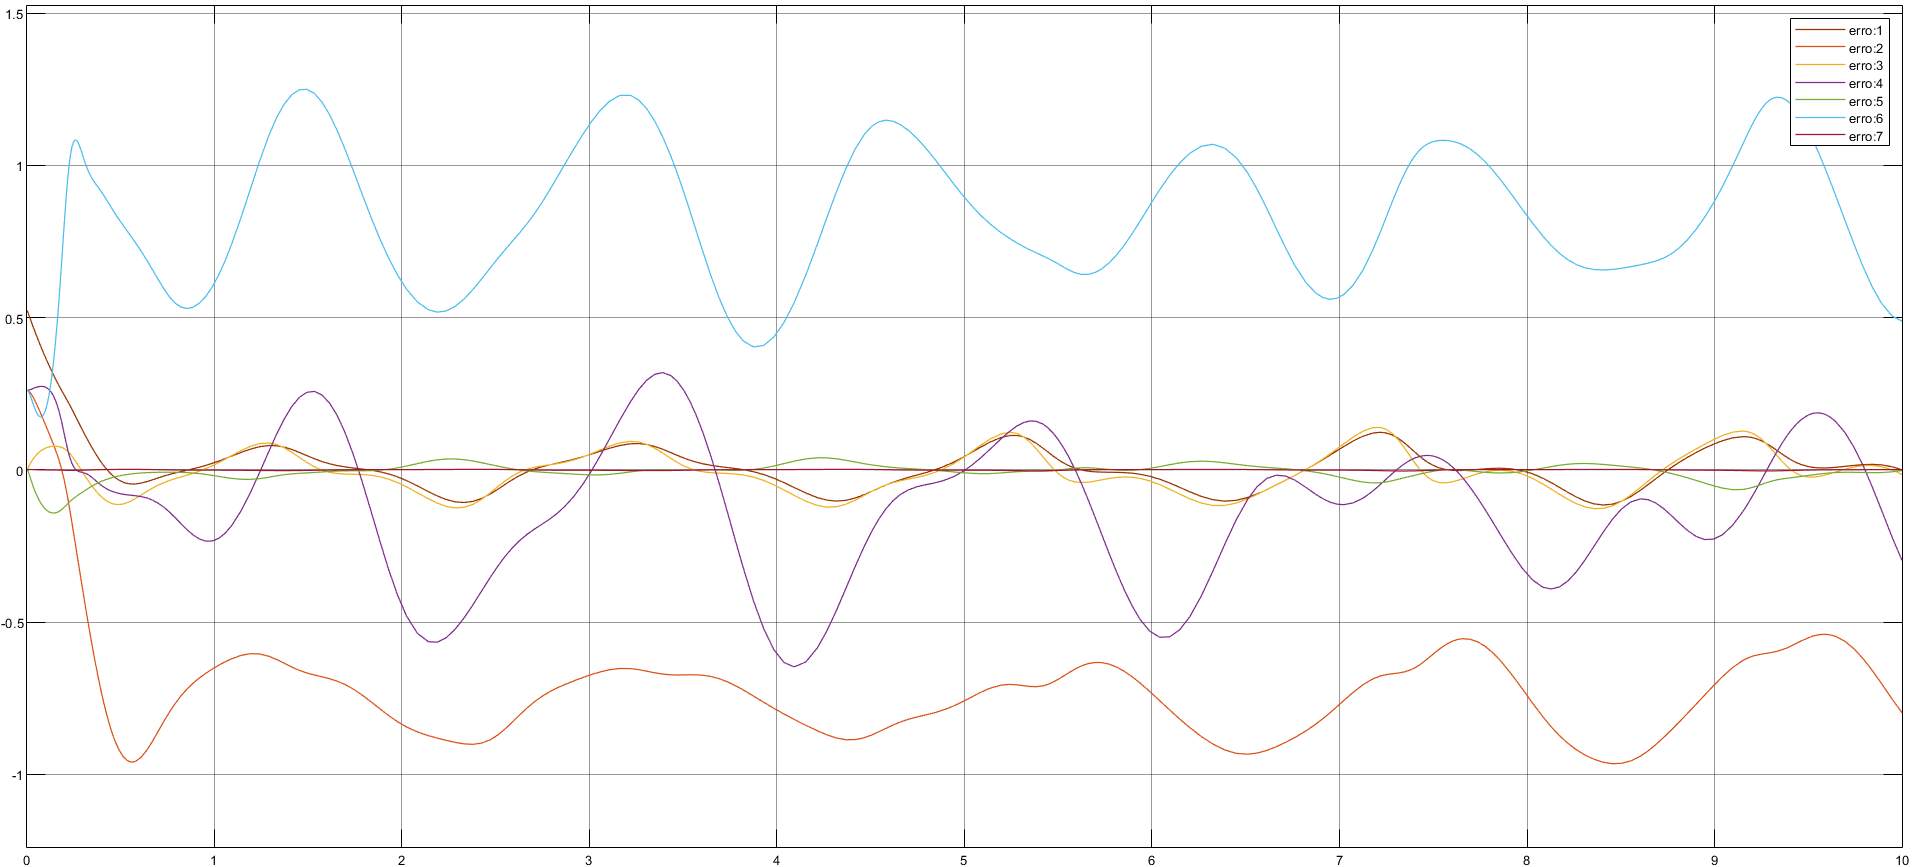
\includegraphics[width=\linewidth]{erro_pd_pi_m.png}
        \caption{Erros de posições das juntas}
        \label{fig:erro_pd_pi_m}
    \end{subfigure}%
    \hfill
    \begin{subfigure}[b]{0.45\textwidth}
        \centering
        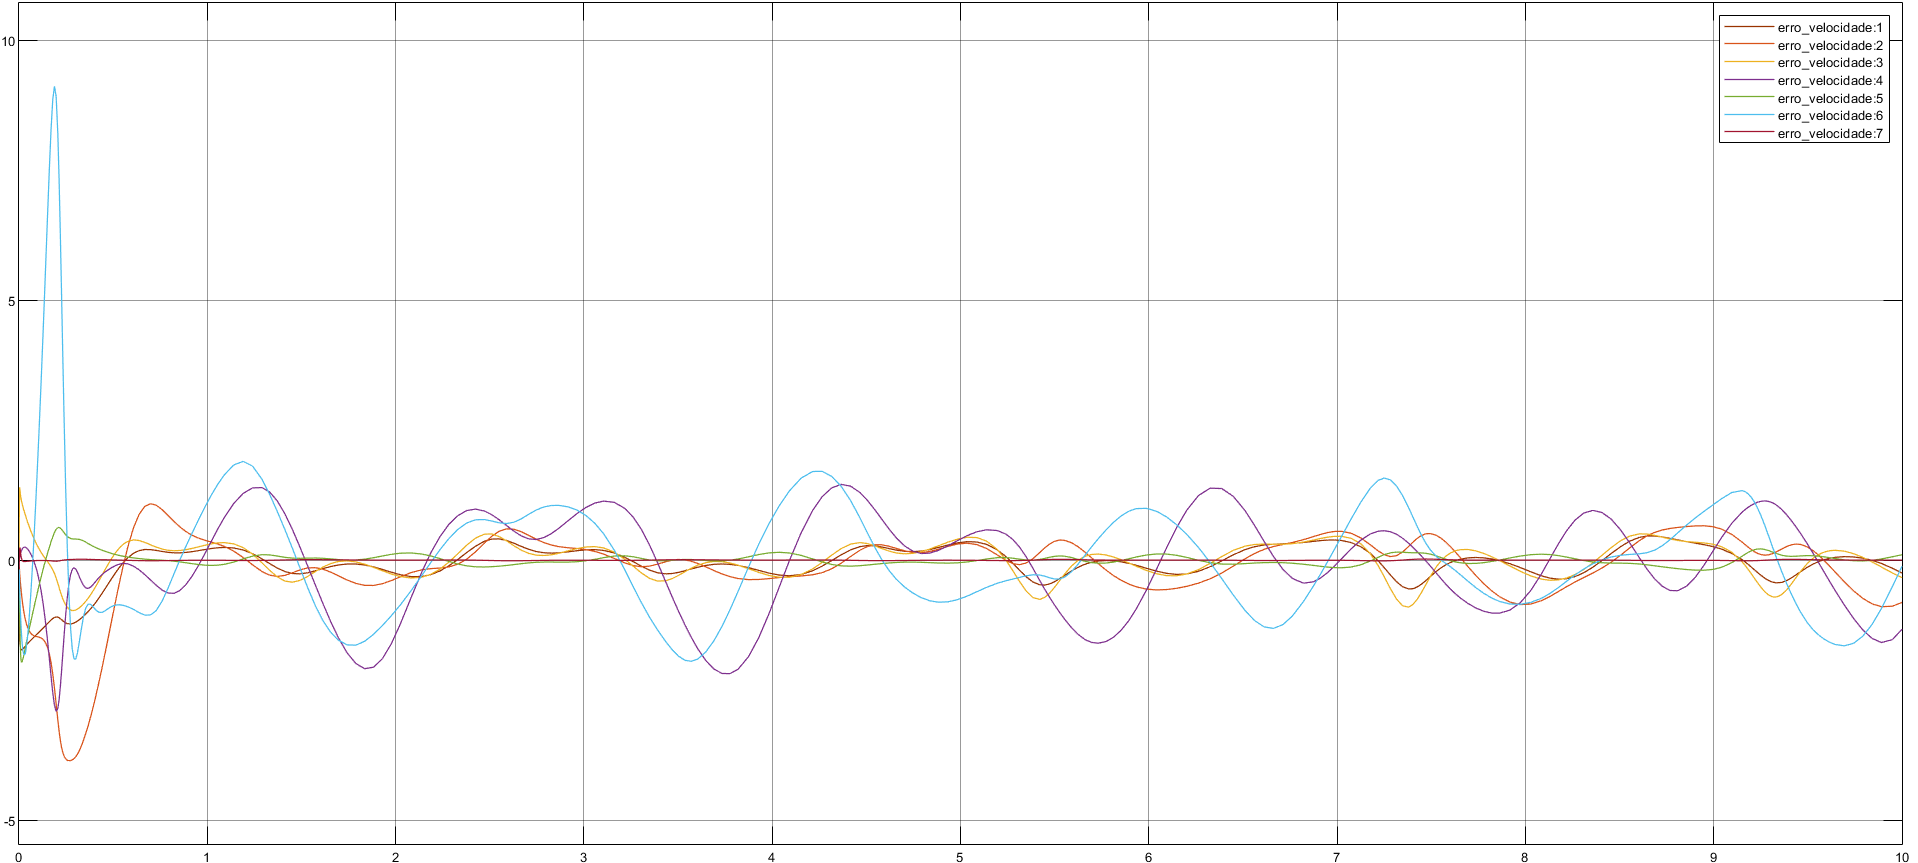
\includegraphics[width=\linewidth]{erro_velocidade_pd_pi_m.png}
        \caption{Erros de velocidades das juntas}
        \label{fig:erro_velocidade_pd_pi_m}
    \end{subfigure}%
    \caption{Controlador PD com massa adicional ($\omega_n = \pi$)}
    \label{fig:imagens_pd_pi_m}
\end{figure}

Ademais, foi feito a simulação com a massa adicional de 10kg para $\omega_n = \pi/2$:

\newpage

\begin{figure}[h!]
    \centering
    \begin{subfigure}[b]{0.45\textwidth}
        \centering
        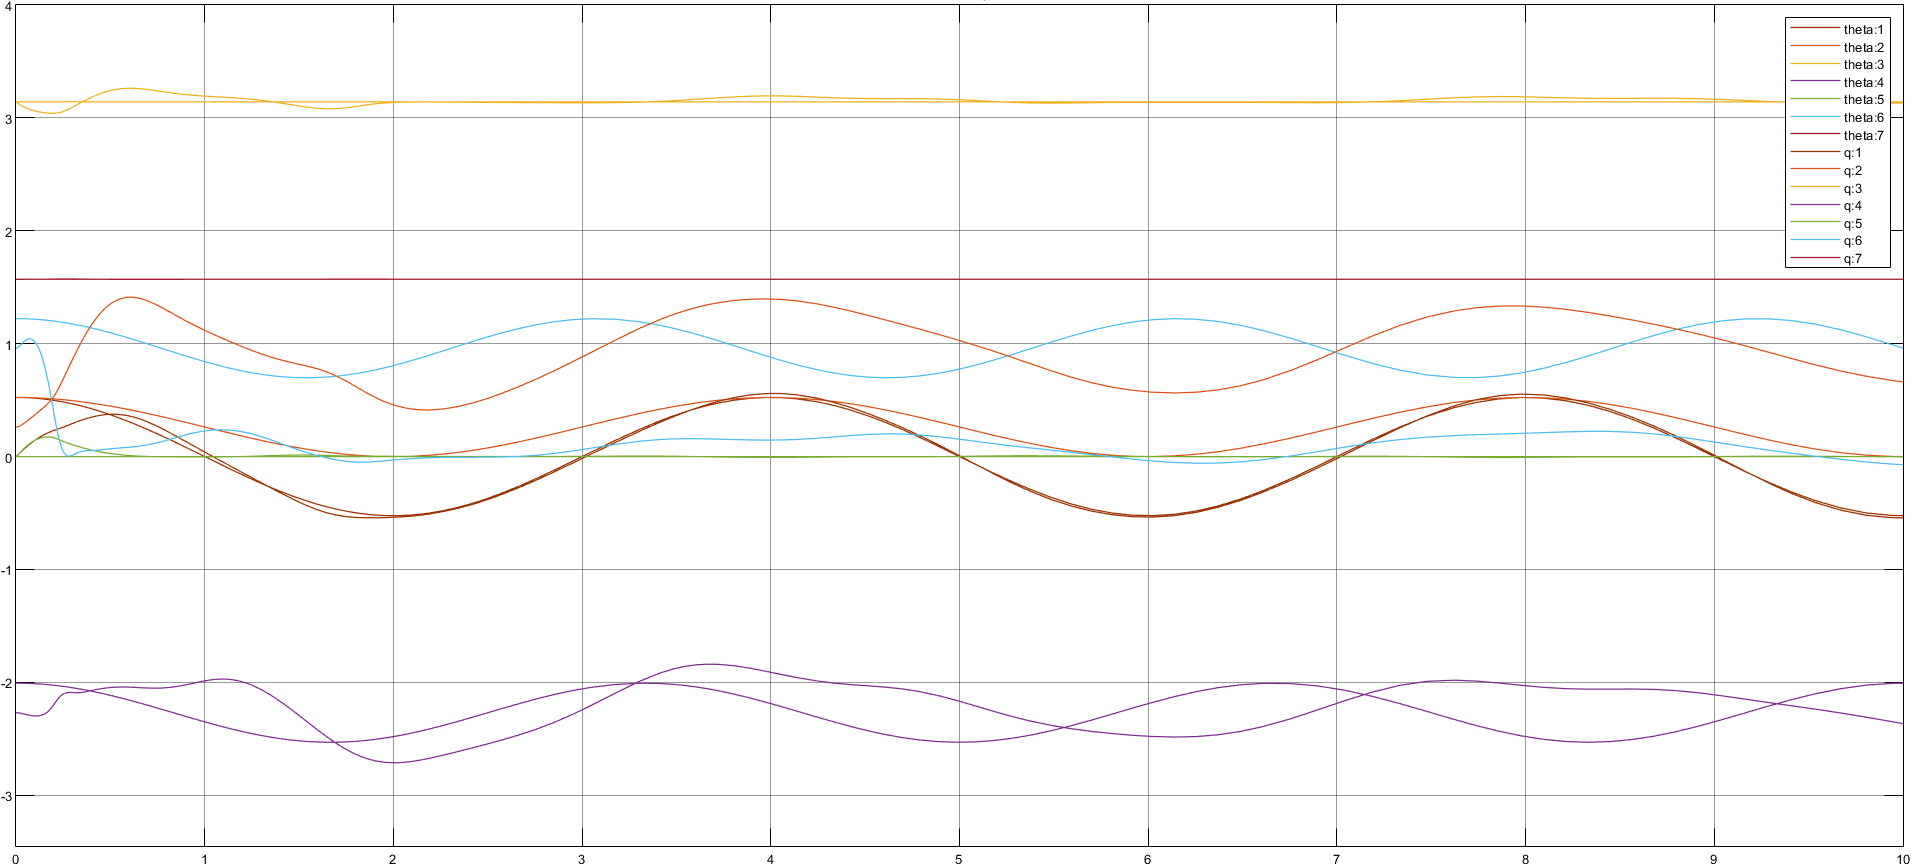
\includegraphics[width=\linewidth]{posicao_pd_pi2_m.png}
        \caption{Posições das juntas}
        \label{fig:posicao_pd_pi2_m}
    \end{subfigure}%
    \hfill
    \begin{subfigure}[b]{0.45\textwidth}
        \centering
        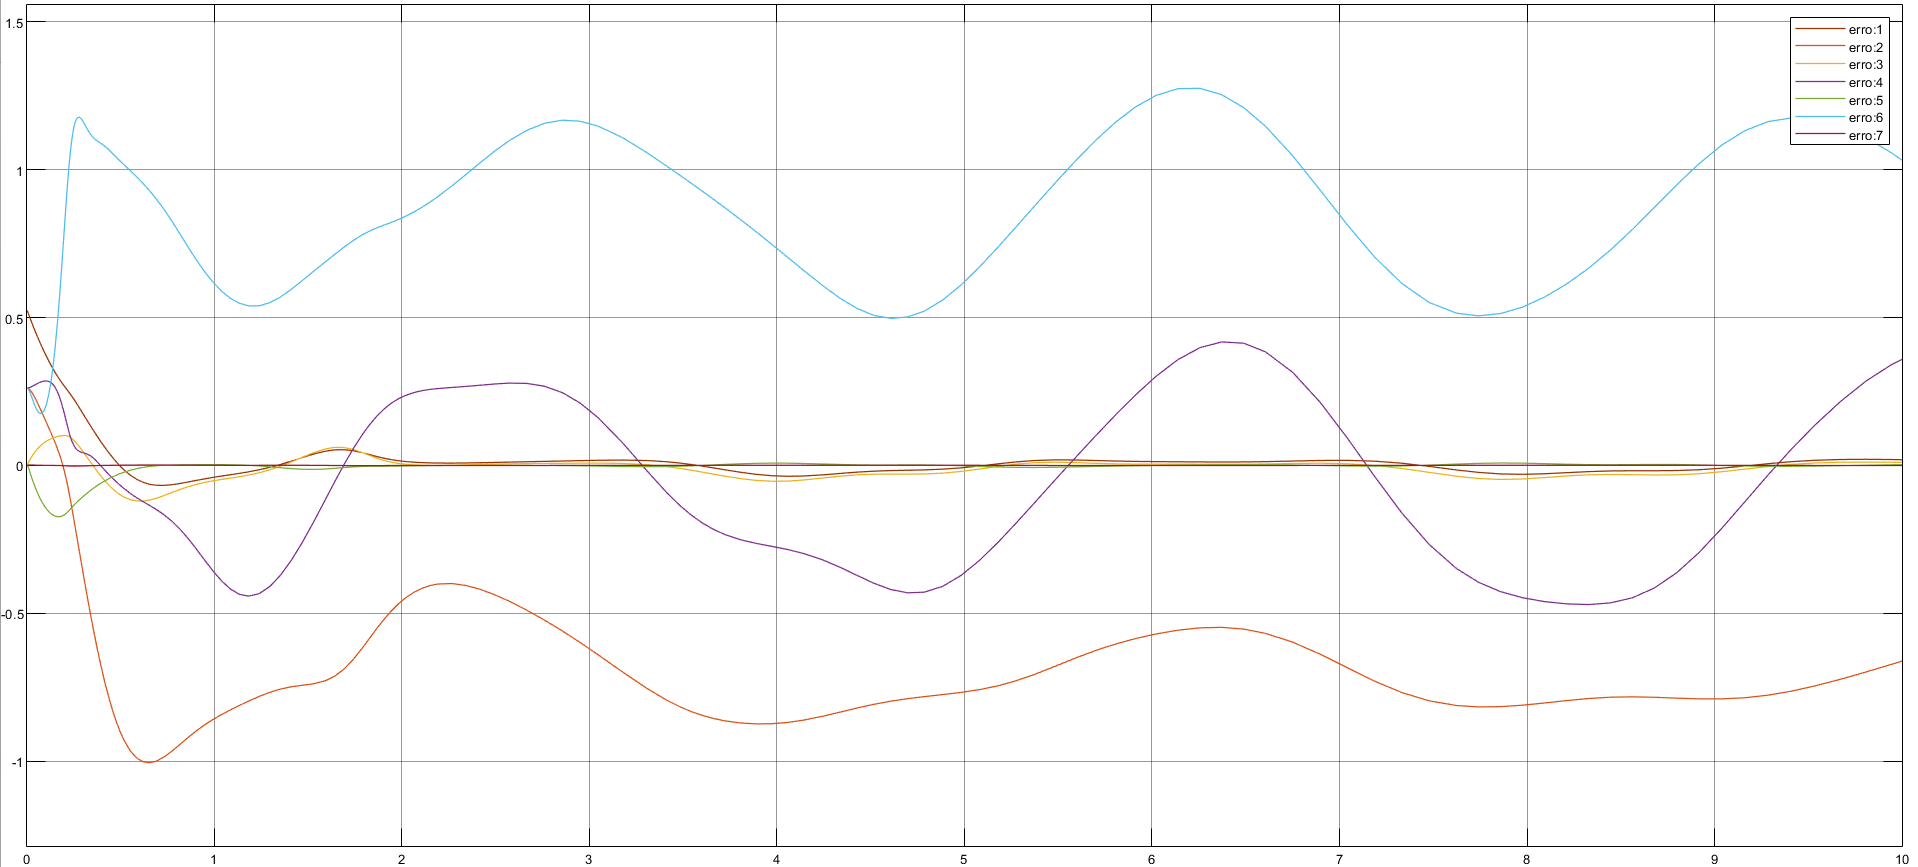
\includegraphics[width=\linewidth]{erro_pd_pi2_m.png}
        \caption{Erros de posições das juntas}
        \label{fig:erro_pd_pi2_m}
    \end{subfigure}%
    \hfill
    \begin{subfigure}[b]{0.45\textwidth}
        \centering
        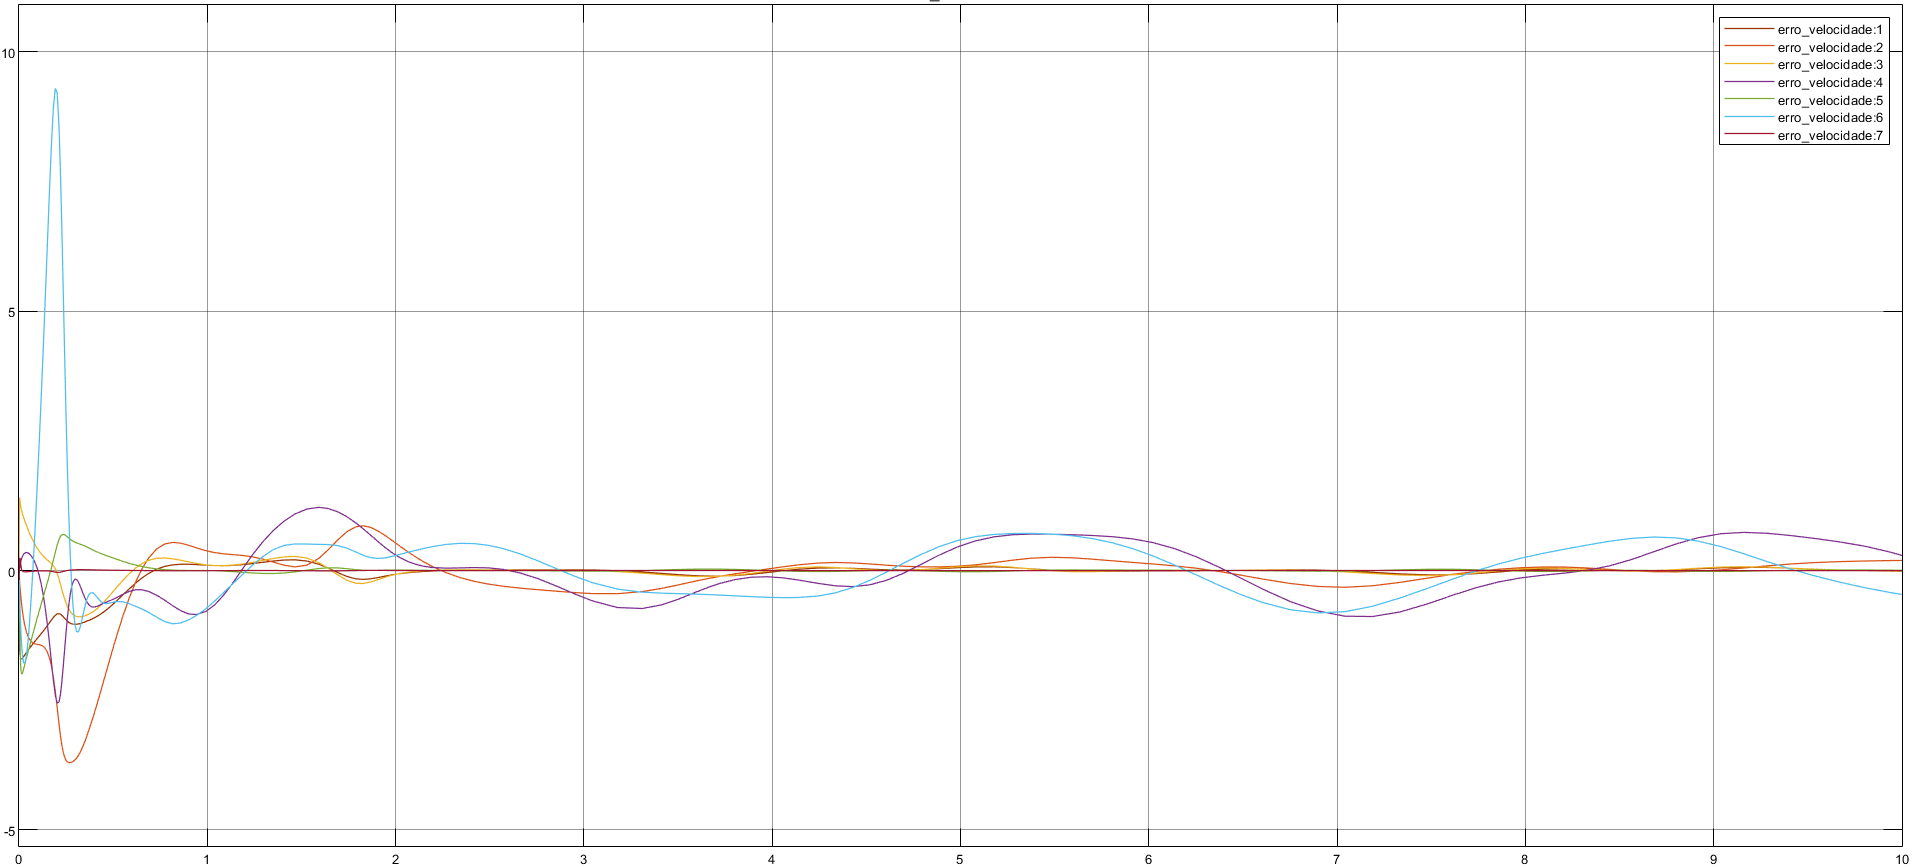
\includegraphics[width=\linewidth]{erro_velocidade_pd_pi2_m.png}
        \caption{Erros de velocidades das juntas}
        \label{fig:erro_velocidade_pd_pi2_m}
    \end{subfigure}%
    \caption{Controlador PD com massa adicional ($\omega_n = \pi/2$)}
    \label{fig:imagens_pd_pi2_m}
\end{figure}

\subsection{Controlador P-PI}

Utilizando o modelo dinâmico do manipulador da equação \eqref{eq:dinamica_simplificada} com as equações do controlador P-PI \eqref{eq:pi_ppi} e \eqref{eq:p_ppi} com $K_a = \bar{M}$, foi obtido o seguinte desenvolvimento:
\begin{equation}
    \tau = \bar{M}\ddot{\theta} + d = -K_d K_p \tilde{\theta} - K_d \dot{\tilde{\theta}} - K_i K_p \int \tilde{\theta} dt - K_i \tilde{\theta} + \bar{M}\ddot{\theta}_d
\end{equation}
em que $d$ é considerado uma perturbação e \(\tilde{\theta} = \theta - \theta_d\).

A equação característica do sistema em malha fechada foi obtido a partir da Transformação de Laplace da equação acima e é escrita como:
\begin{equation}
p_c(s) = \bar{M}s^3 + K_d s^2 + (K_d K_p + K_i)s + K_i K_p = 0
\end{equation}
A partir disso é desejado a seguinte equação característica respeitando os parâmetros de projeto:
\begin{equation}
    p_c(s) = \bar{M}(s^2 + 100s + 2500)(s + 10) = \bar{M}(s^3 + 110s^2 + 3500s + 25000)
\end{equation}
com isso temos que $K_d = 110 \bar{M}$, $K_p = 10.8271 \bar{M}$ e $K_i = 2309 \bar{M}$.

A seguir temos o diagrama do controlador P-PI implementado no Simulink:

\newpage
    
\begin{figure}[h]
    \centering
    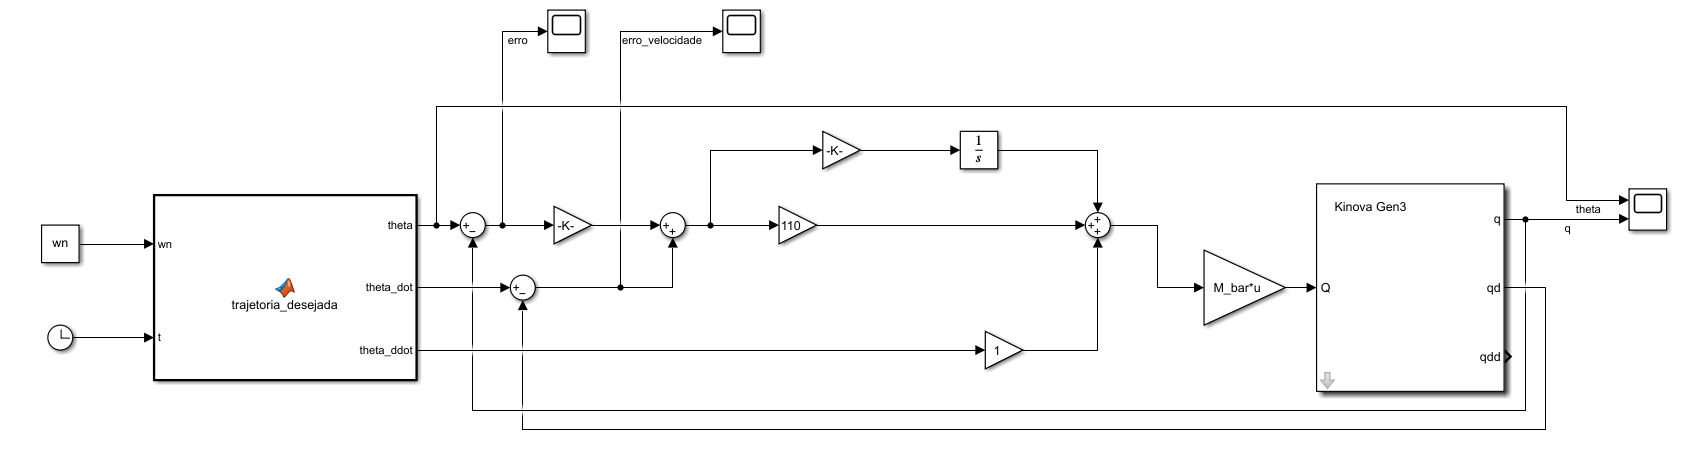
\includegraphics[scale=0.5]{diagrama_ppi.png}
    \caption{Diagrama do controlador P-PI}
\end{figure}

Além disso, foi avaliado esse controlador para um intervalo de $2\pi$ segundos com um $\omega_n = \pi$.
Isso foi feito observando as posições das juntas,
o erro entre as posições das juntas e as posições das trajetórias desejadas e
o erro entre as velocidades das juntas e as velocidades das trajetórias desejadas.
A seguir temos os gráficos:

\begin{figure}[h!]
    \centering
    \begin{subfigure}[b]{0.49\textwidth}
        \centering
        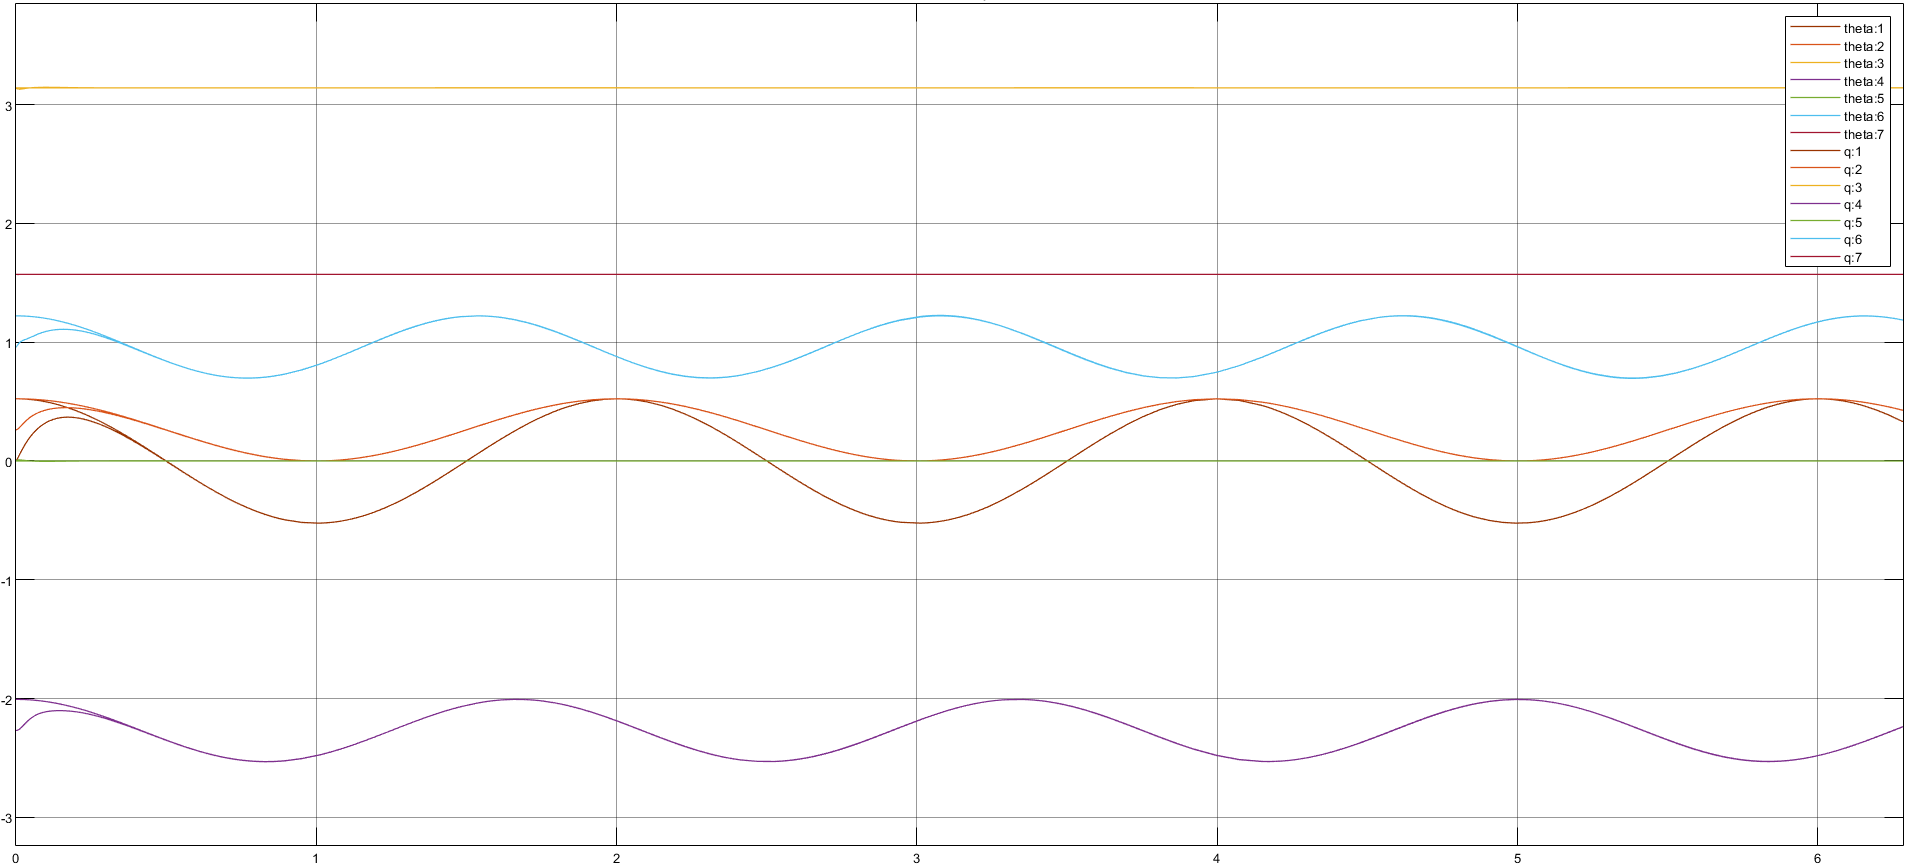
\includegraphics[width=\linewidth]{posicao_ppi_pi.png}
        \caption{Posições das juntas}
        \label{fig:posicao_ppi_pi}
    \end{subfigure}%
    \hfill
    \begin{subfigure}[b]{0.49\textwidth}
        \centering
        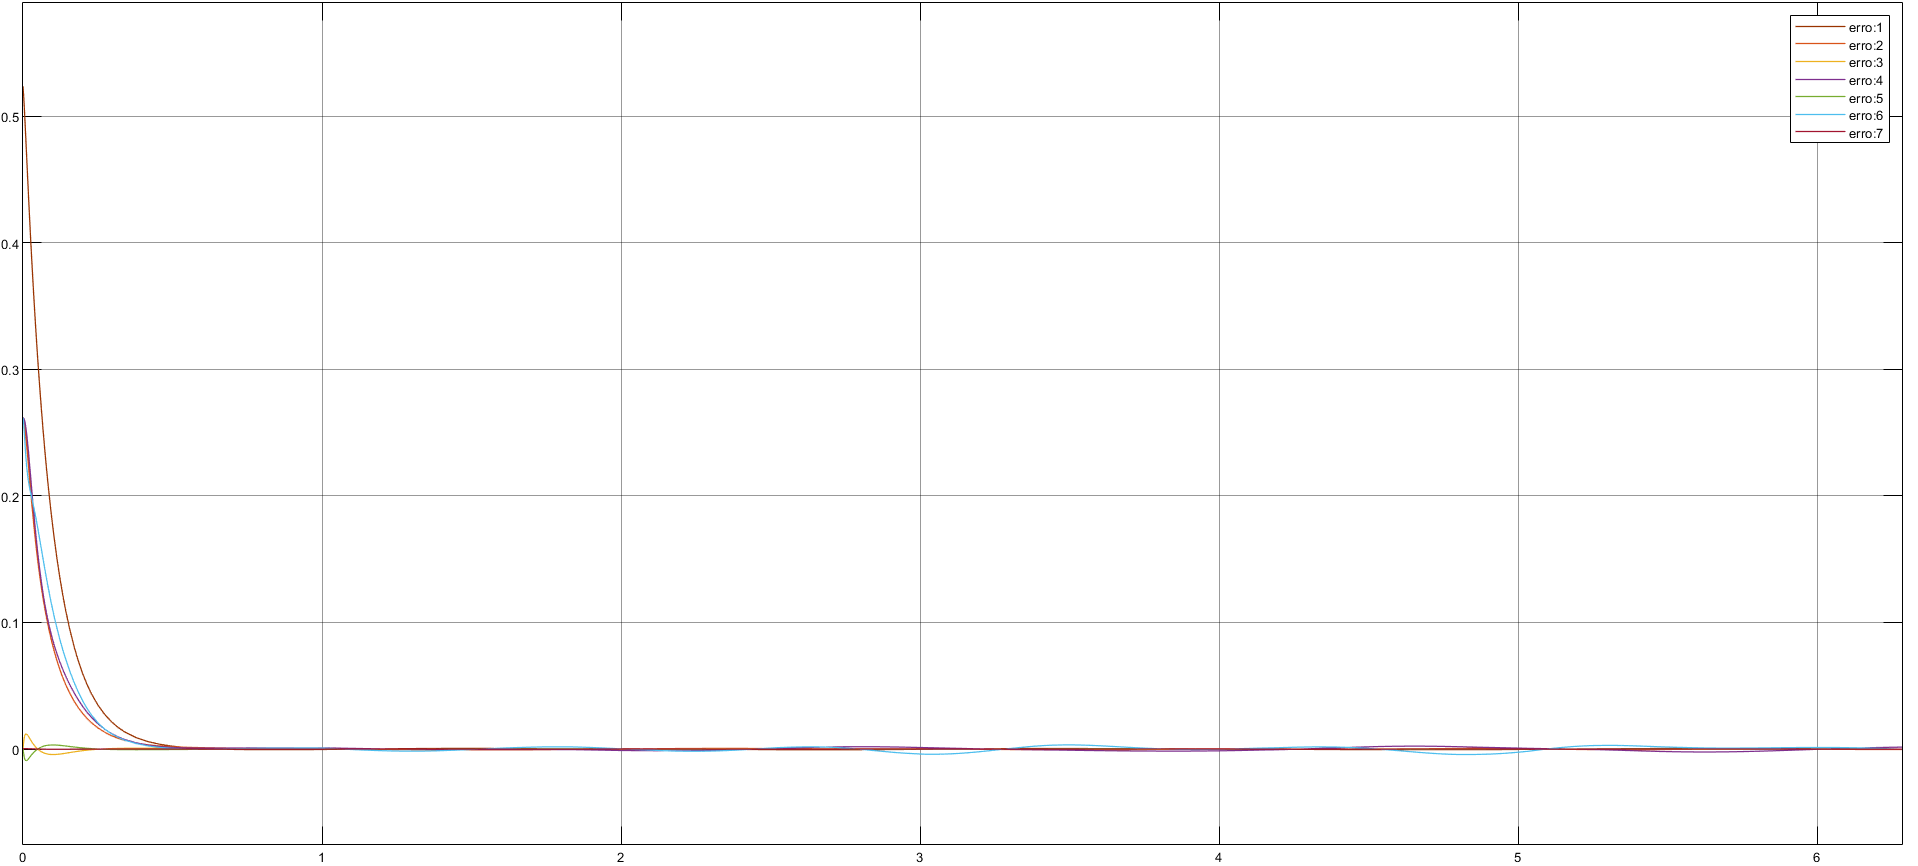
\includegraphics[width=\linewidth]{erro_ppi_pi.png}
        \caption{Erros de posições das juntas}
        \label{fig:erro_ppi_pi}
    \end{subfigure}%
    \hfill
    \begin{subfigure}[b]{0.49\textwidth}
        \centering
        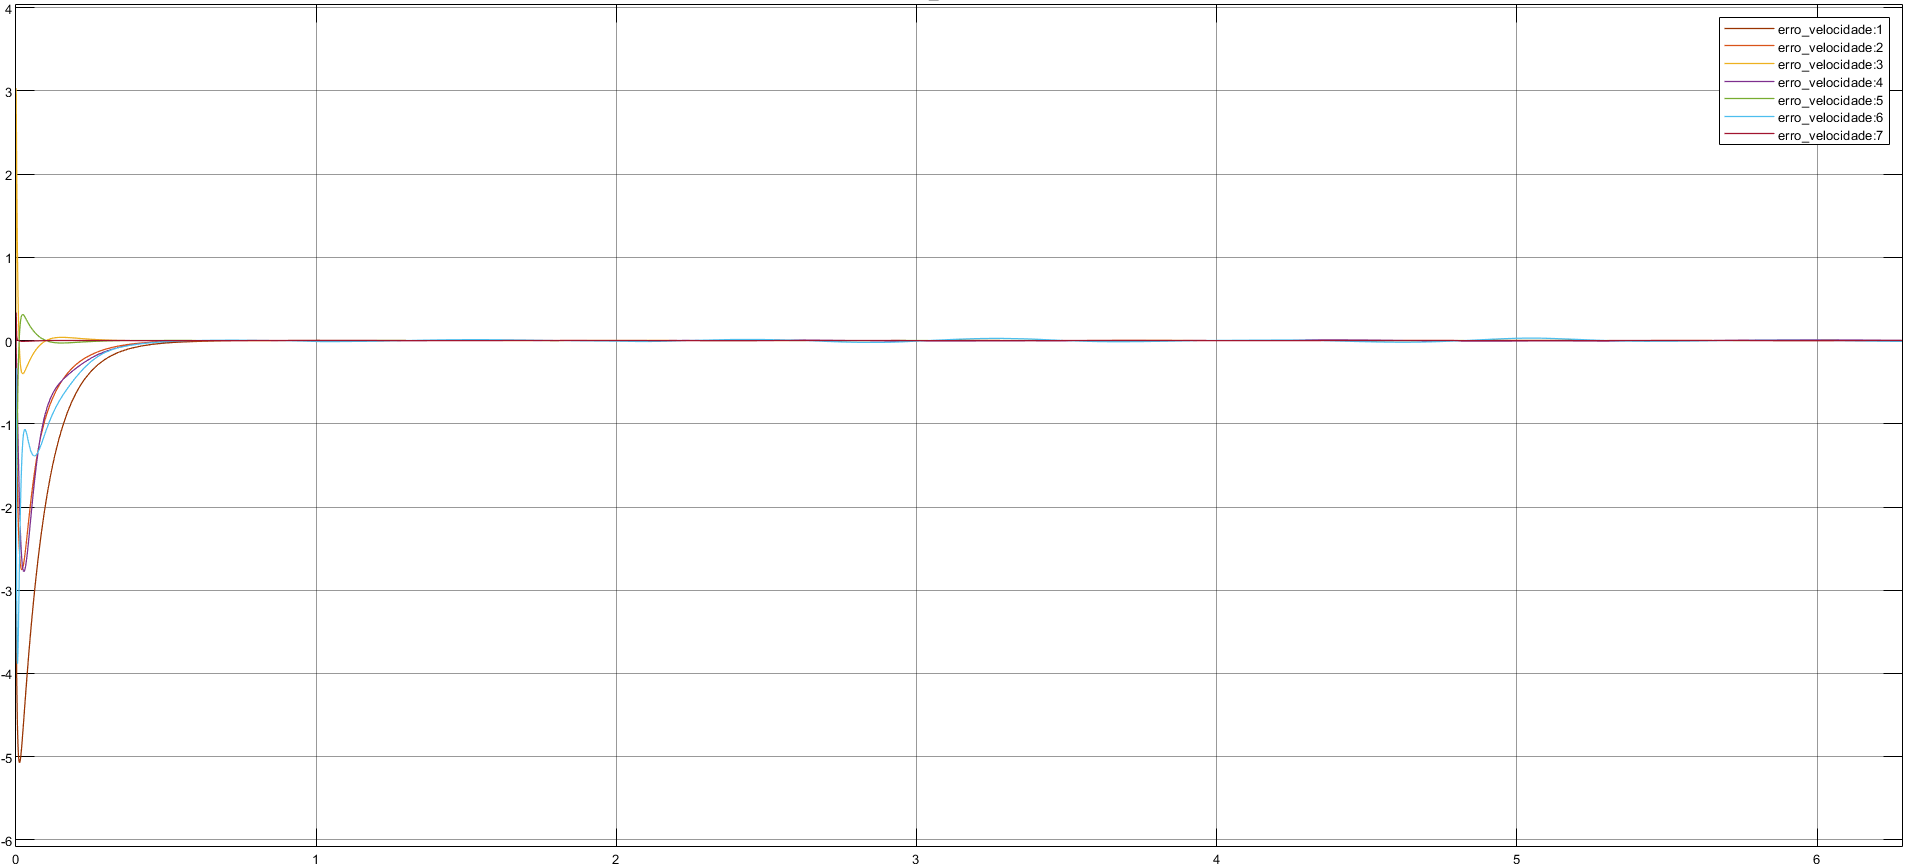
\includegraphics[width=\linewidth]{erro_velocidade_ppi_pi.png}
        \caption{Erros de velocidades das juntas}
        \label{fig:erro_velocidade_ppi_pi}
    \end{subfigure}%
    \caption{Controlador P-PI ($\omega_n = \pi$)}
    \label{fig:imagens_ppi_pi}
\end{figure}
Isso também foi feito para $\omega_n = \pi/2$. Obtendo os seguintes resultados:

\newpage

\begin{figure}[h!]
    \centering
    \begin{subfigure}[b]{0.49\textwidth}
        \centering
        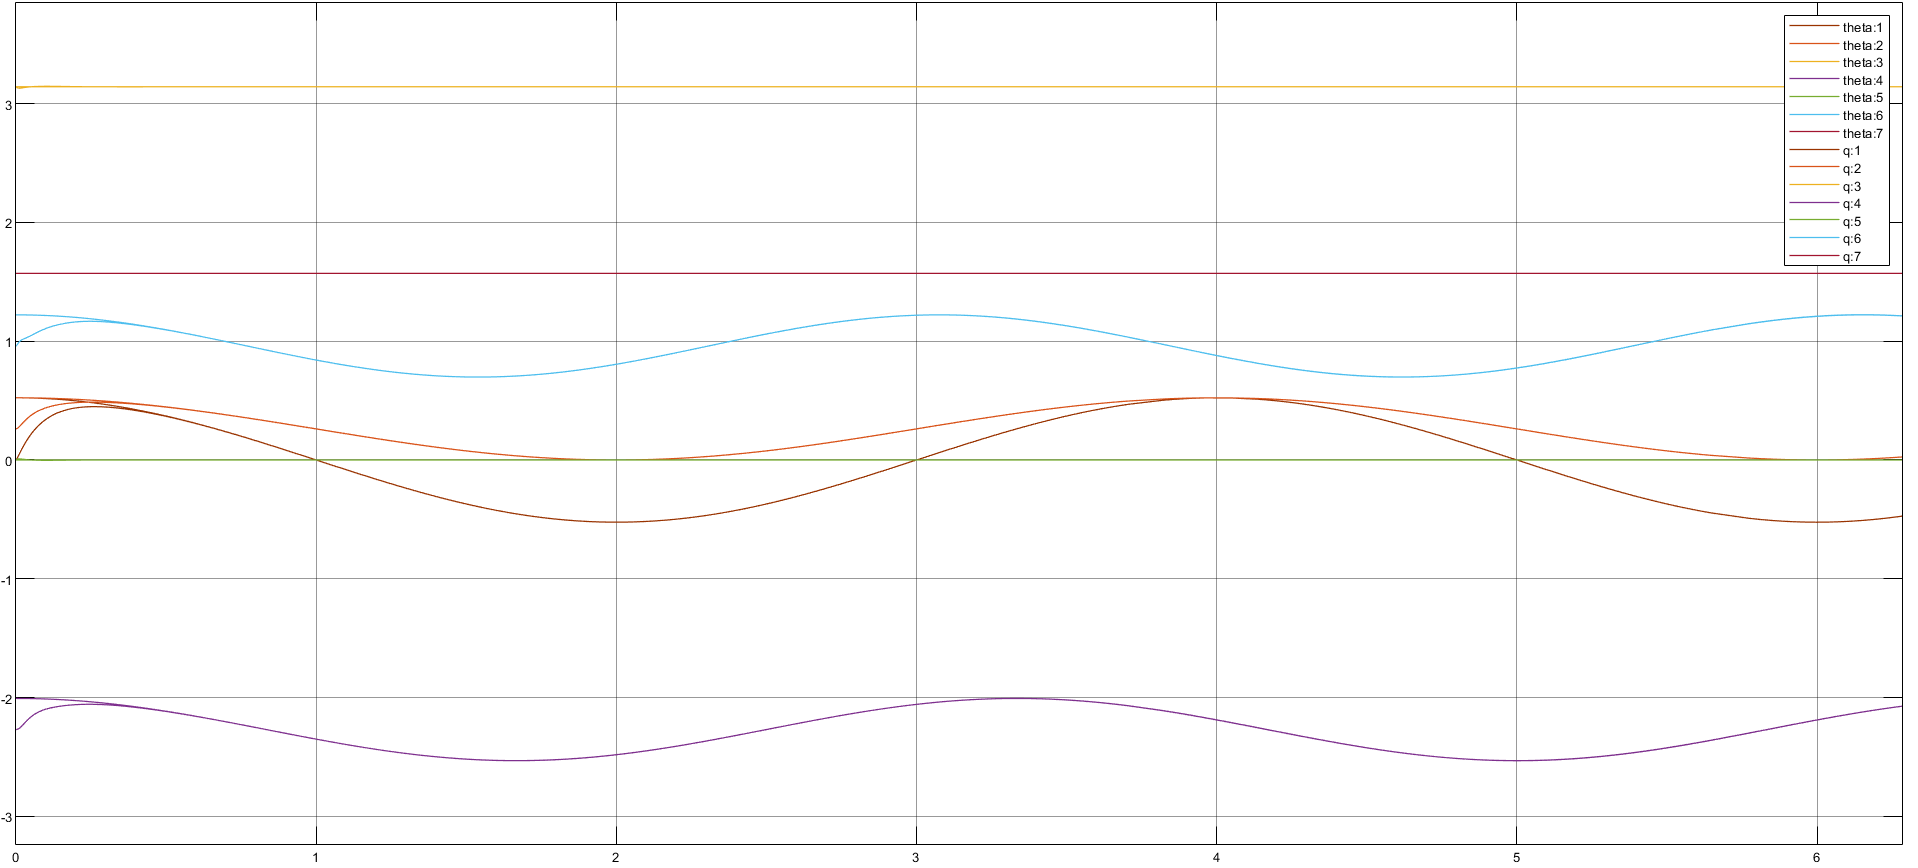
\includegraphics[width=\linewidth]{posicao_ppi_pi2.png}
        \caption{Posições das juntas}
        \label{fig:posicao_ppi_pi2}
    \end{subfigure}%
    \hfill
    \begin{subfigure}[b]{0.49\textwidth}
        \centering
        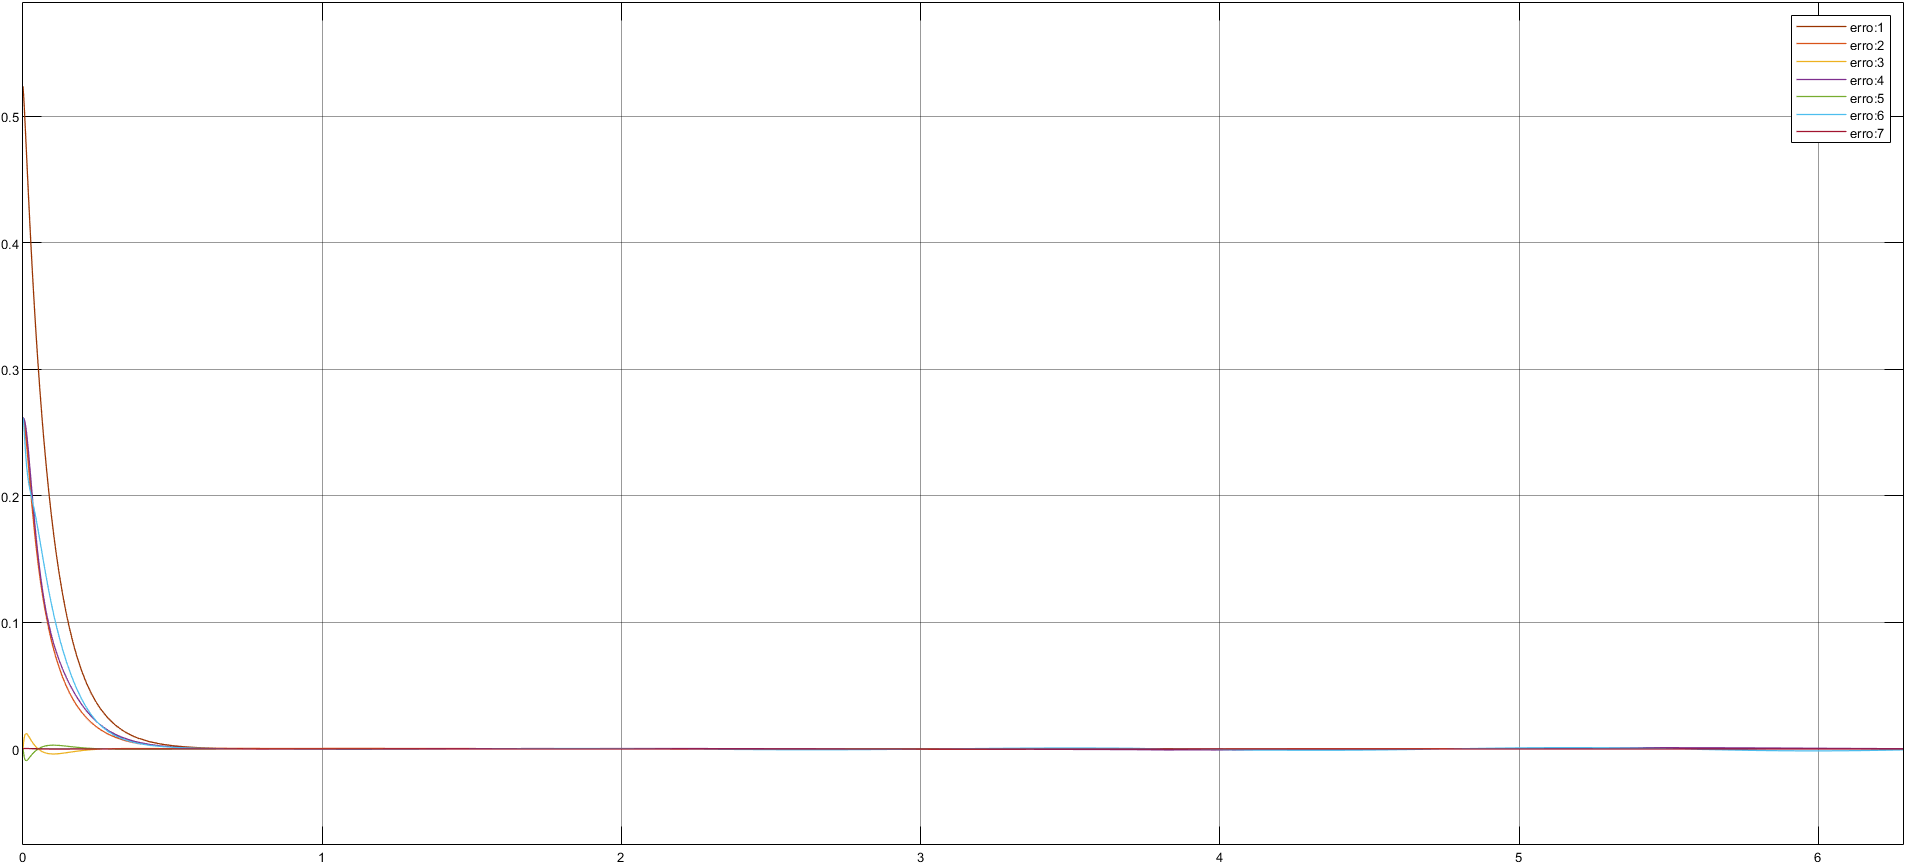
\includegraphics[width=\linewidth]{erro_ppi_pi2.png}
        \caption{Erros de posições das juntas}
        \label{fig:erro_ppi_pi2}
    \end{subfigure}%
    \hfill
    \begin{subfigure}[b]{0.49\textwidth}
        \centering
        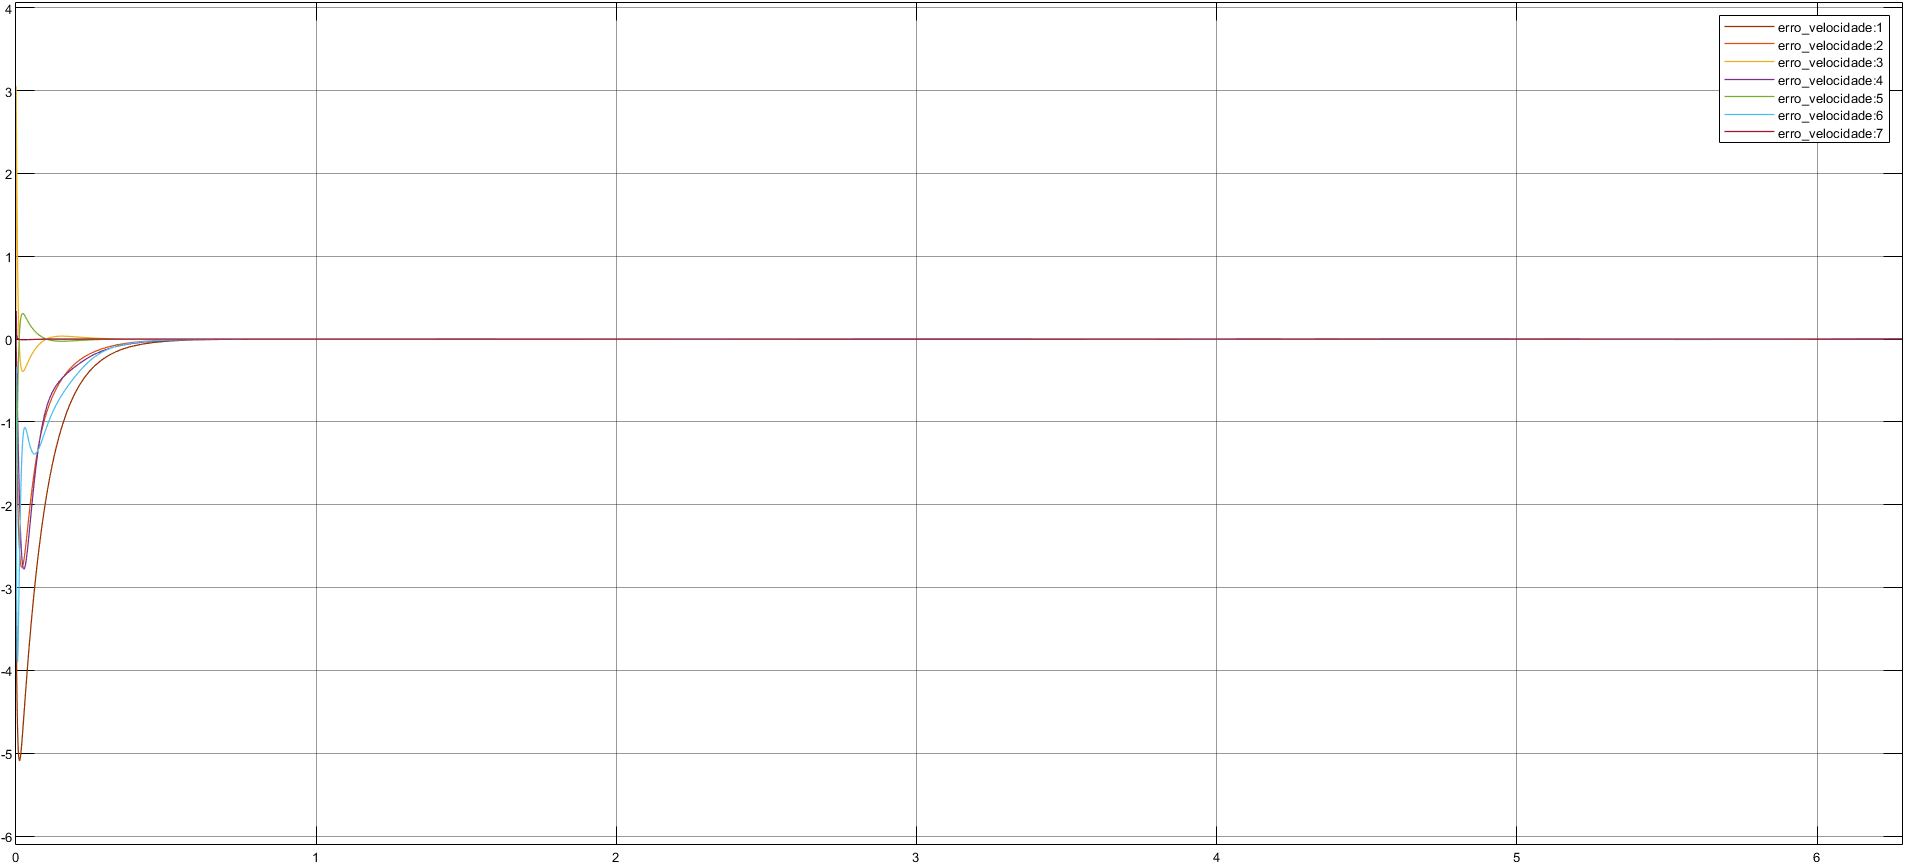
\includegraphics[width=\linewidth]{erro_velocidade_ppi_pi2.png}
        \caption{Erros de velocidades das juntas}
        \label{fig:erro_velocidade_ppi_pi2}
    \end{subfigure}%
    \caption{Controlador P-PI ($\omega_n = \pi/2$)}
    \label{fig:imagens_ppi_pi2}
\end{figure}

Além disso, foi feito a simulação com a massa adicional de 10kg para $\omega_n = \pi$:

\begin{figure}[h!]
    \centering
    \begin{subfigure}[b]{0.49\textwidth}
        \centering
        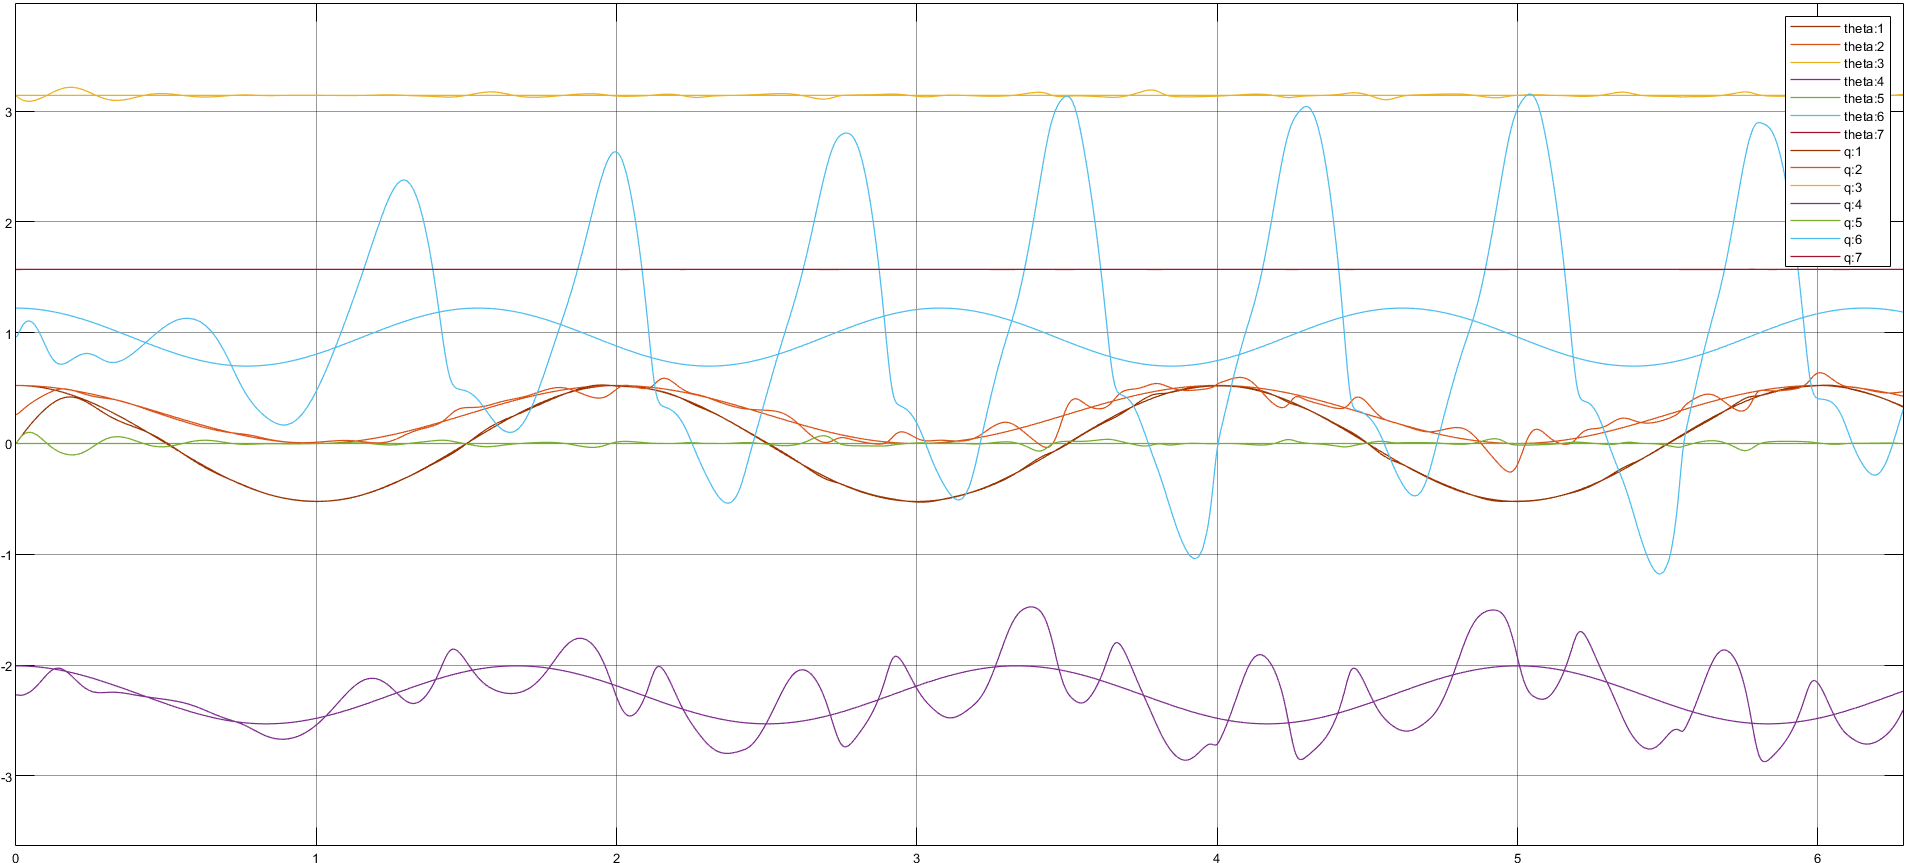
\includegraphics[width=\linewidth]{posicao_ppi_pi_m.png}
        \caption{Posições das juntas}
        \label{fig:posicao_ppi_pi_m}
    \end{subfigure}%
    \hfill
    \begin{subfigure}[b]{0.49\textwidth}
        \centering
        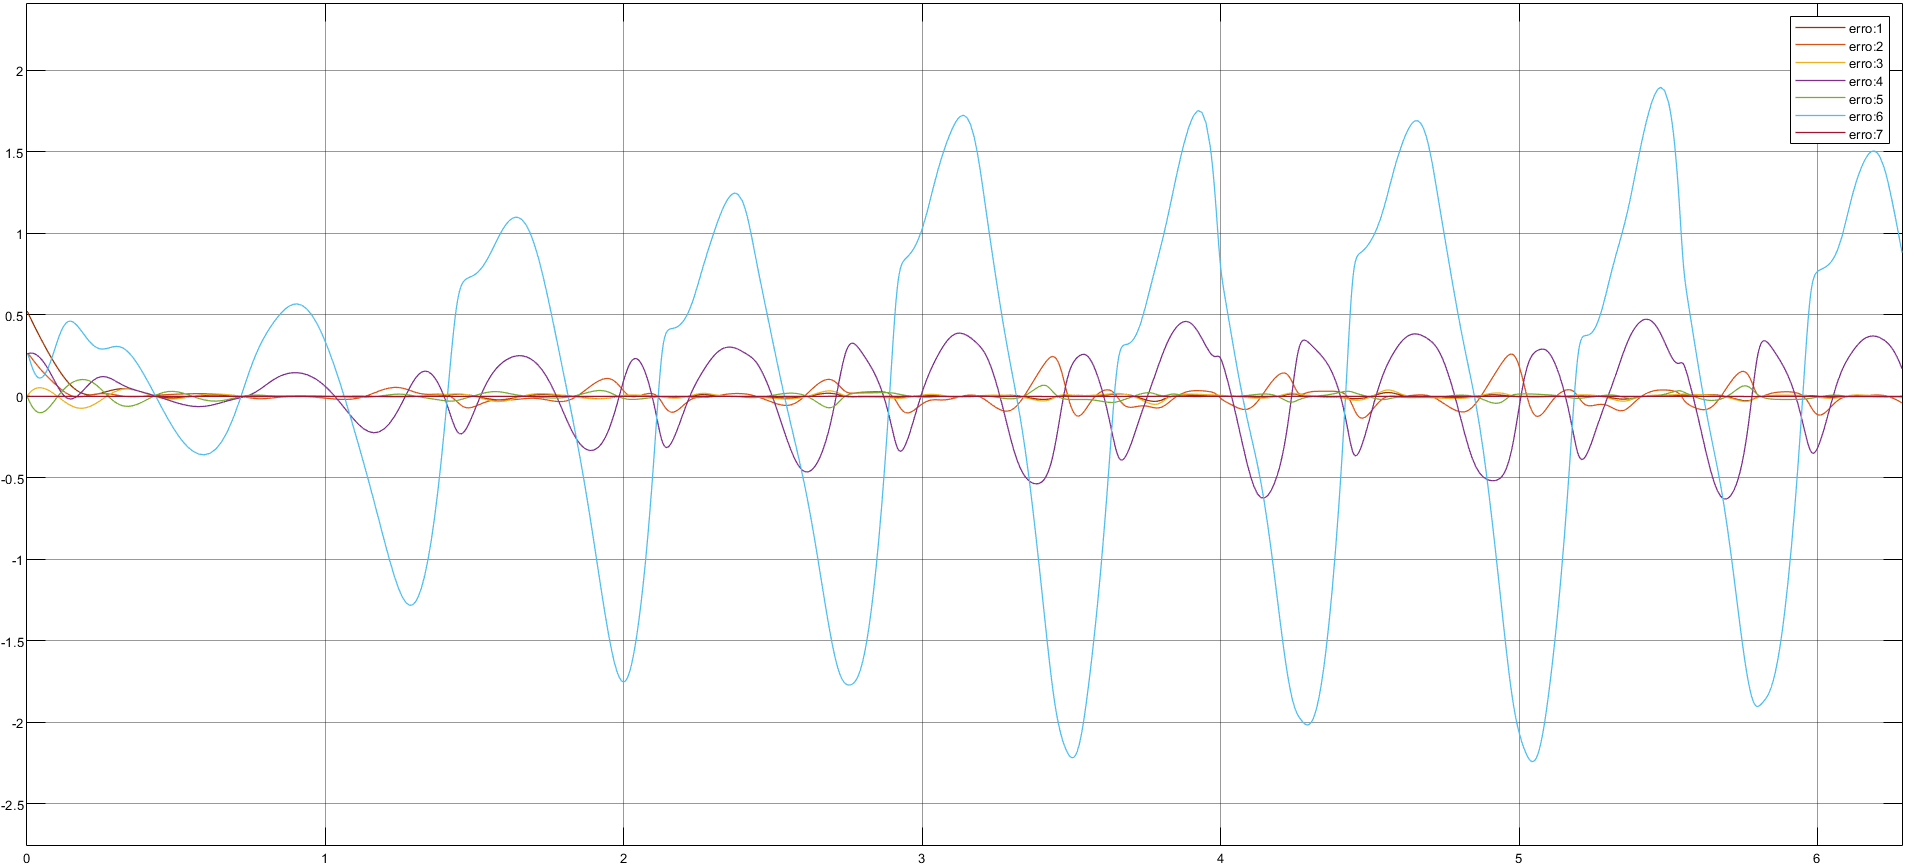
\includegraphics[width=\linewidth]{erro_ppi_pi_m.png}
        \caption{Erros de posições das juntas}
        \label{fig:erro_ppi_pi_m}
    \end{subfigure}%
    \hfill
    \begin{subfigure}[b]{0.49\textwidth}
        \centering
        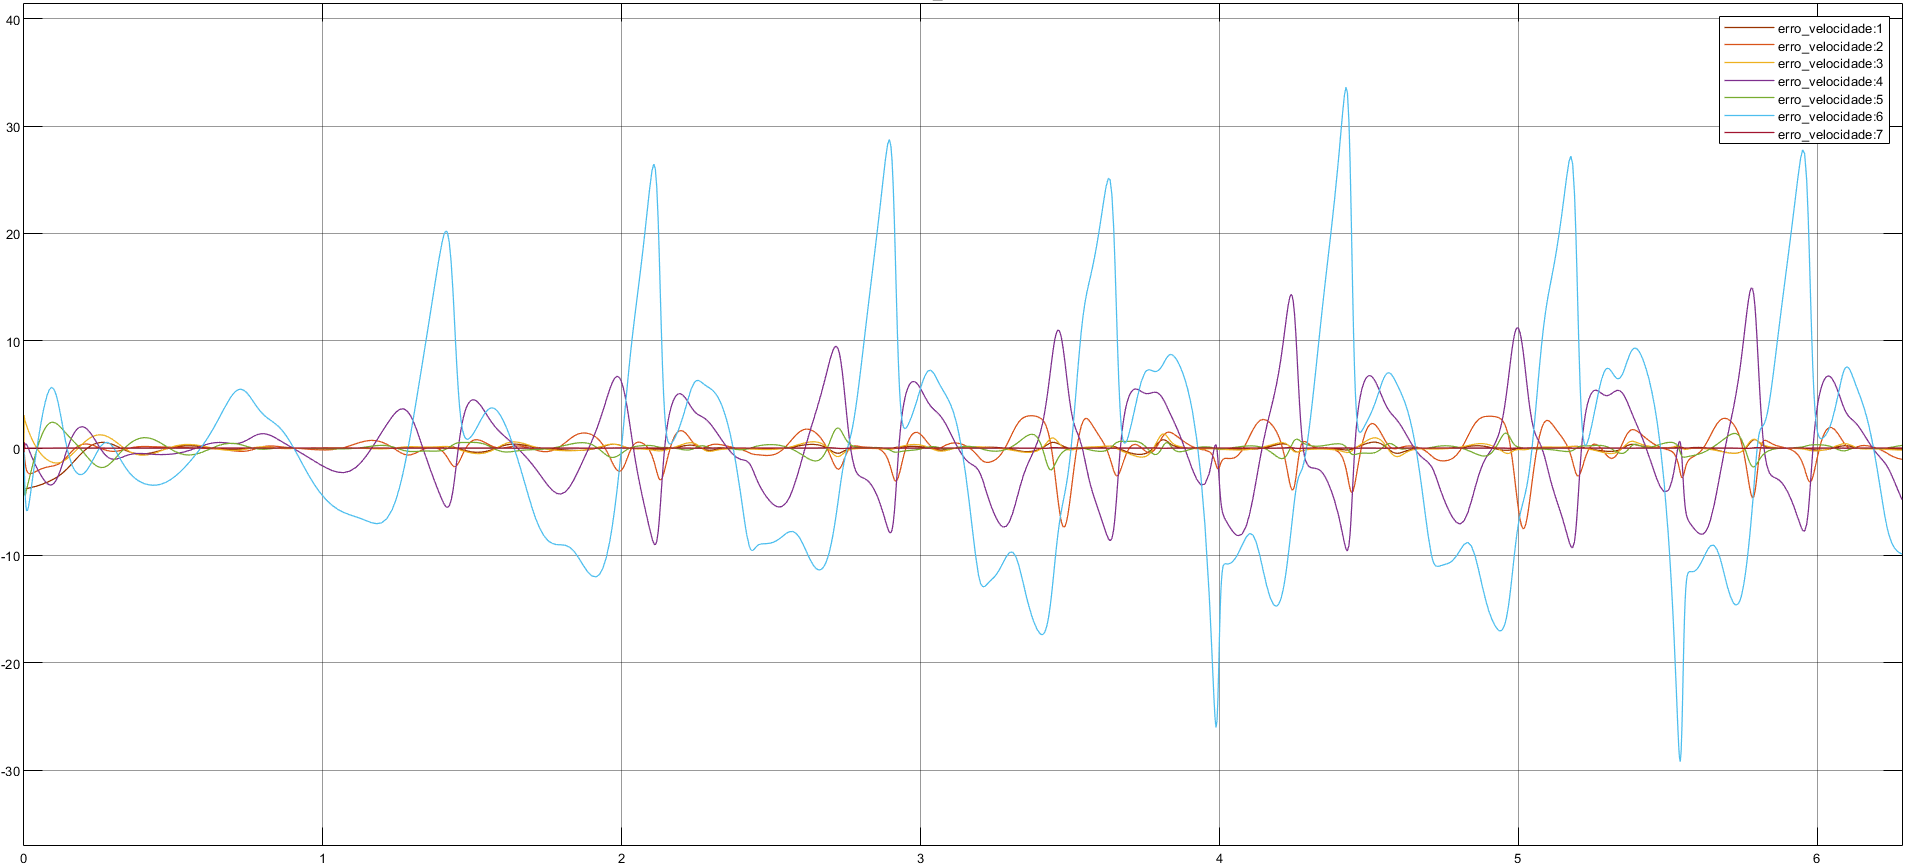
\includegraphics[width=\linewidth]{erro_velocidade_ppi_pi_m.png}
        \caption{Erros de velocidades das juntas}
        \label{fig:erro_velocidade_ppi_pi_m}
    \end{subfigure}%
    \caption{Controlador P-PI com massa adicional ($\omega_n = \pi$)}
    \label{fig:imagens_ppi_pi_m}
\end{figure}

Ademais, foi feito a simulação com a massa adicional de 10kg para $\omega_n = \pi/2$:

\begin{figure}[h!]
    \centering
    \begin{subfigure}[b]{0.49\textwidth}
        \centering
        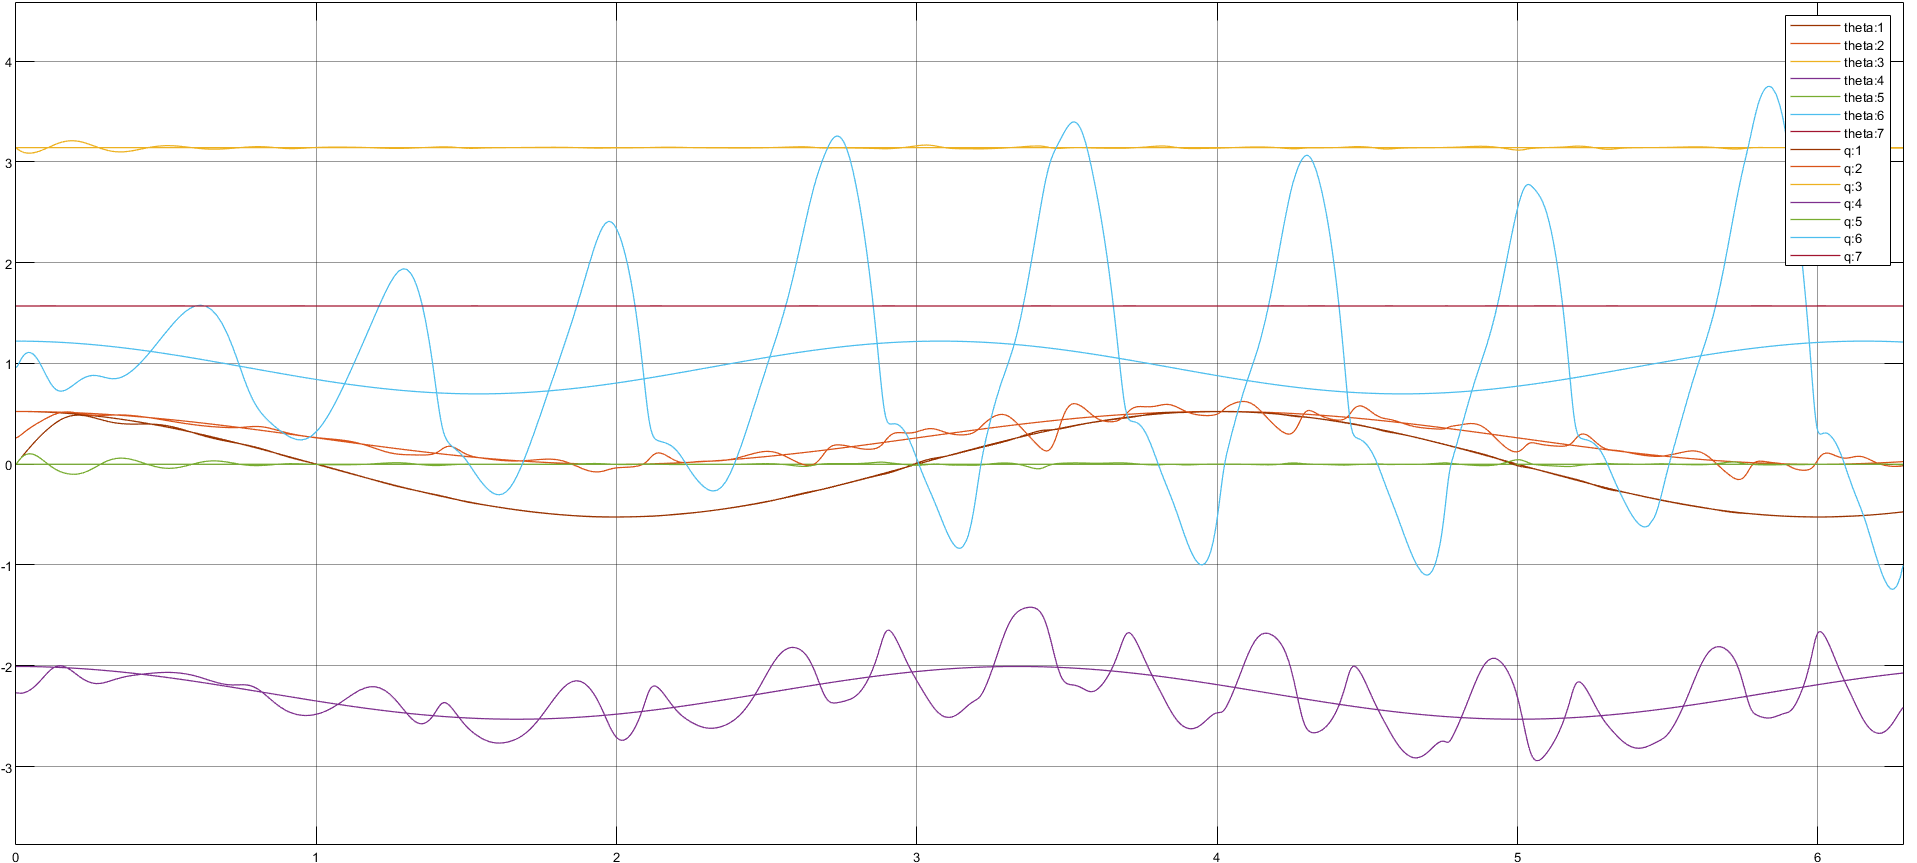
\includegraphics[width=\linewidth]{posicao_ppi_pi2_m.png}
        \caption{Posições das juntas}
        \label{fig:posicao_ppi_pi2_m}
    \end{subfigure}%
    \hfill
    \begin{subfigure}[b]{0.49\textwidth}
        \centering
        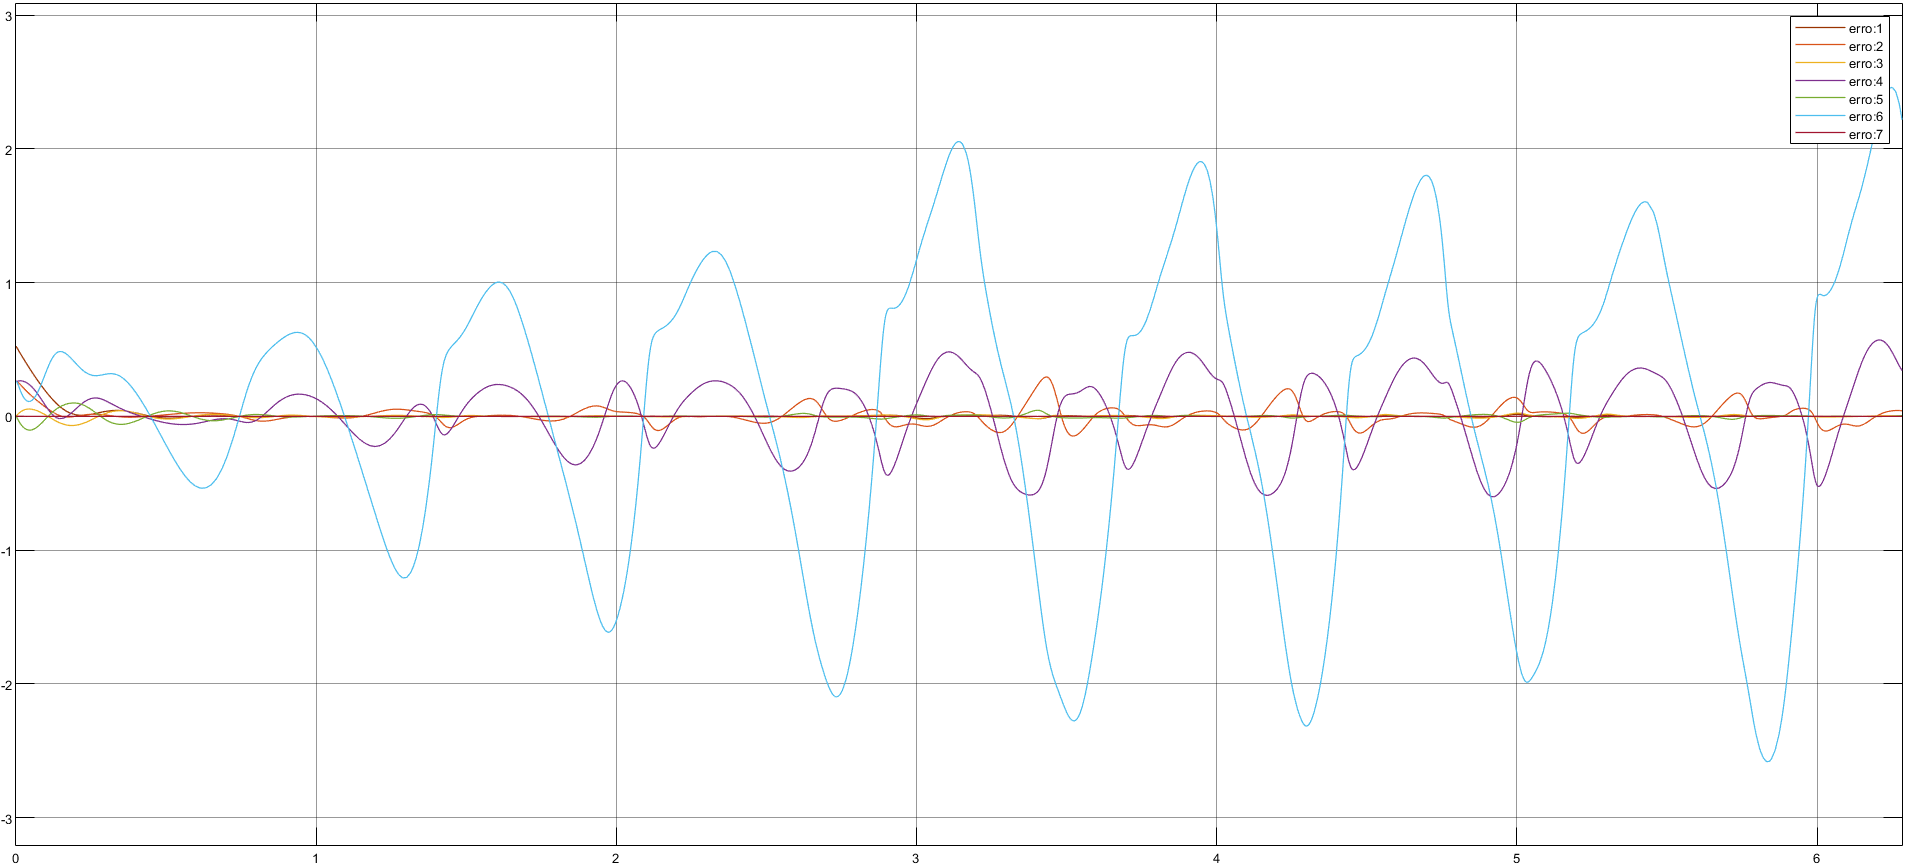
\includegraphics[width=\linewidth]{erro_ppi_pi2_m.png}
        \caption{Erros de posições das juntas}
        \label{fig:erro_ppi_pi2_m}
    \end{subfigure}%
    \hfill
    \begin{subfigure}[b]{0.49\textwidth}
        \centering
        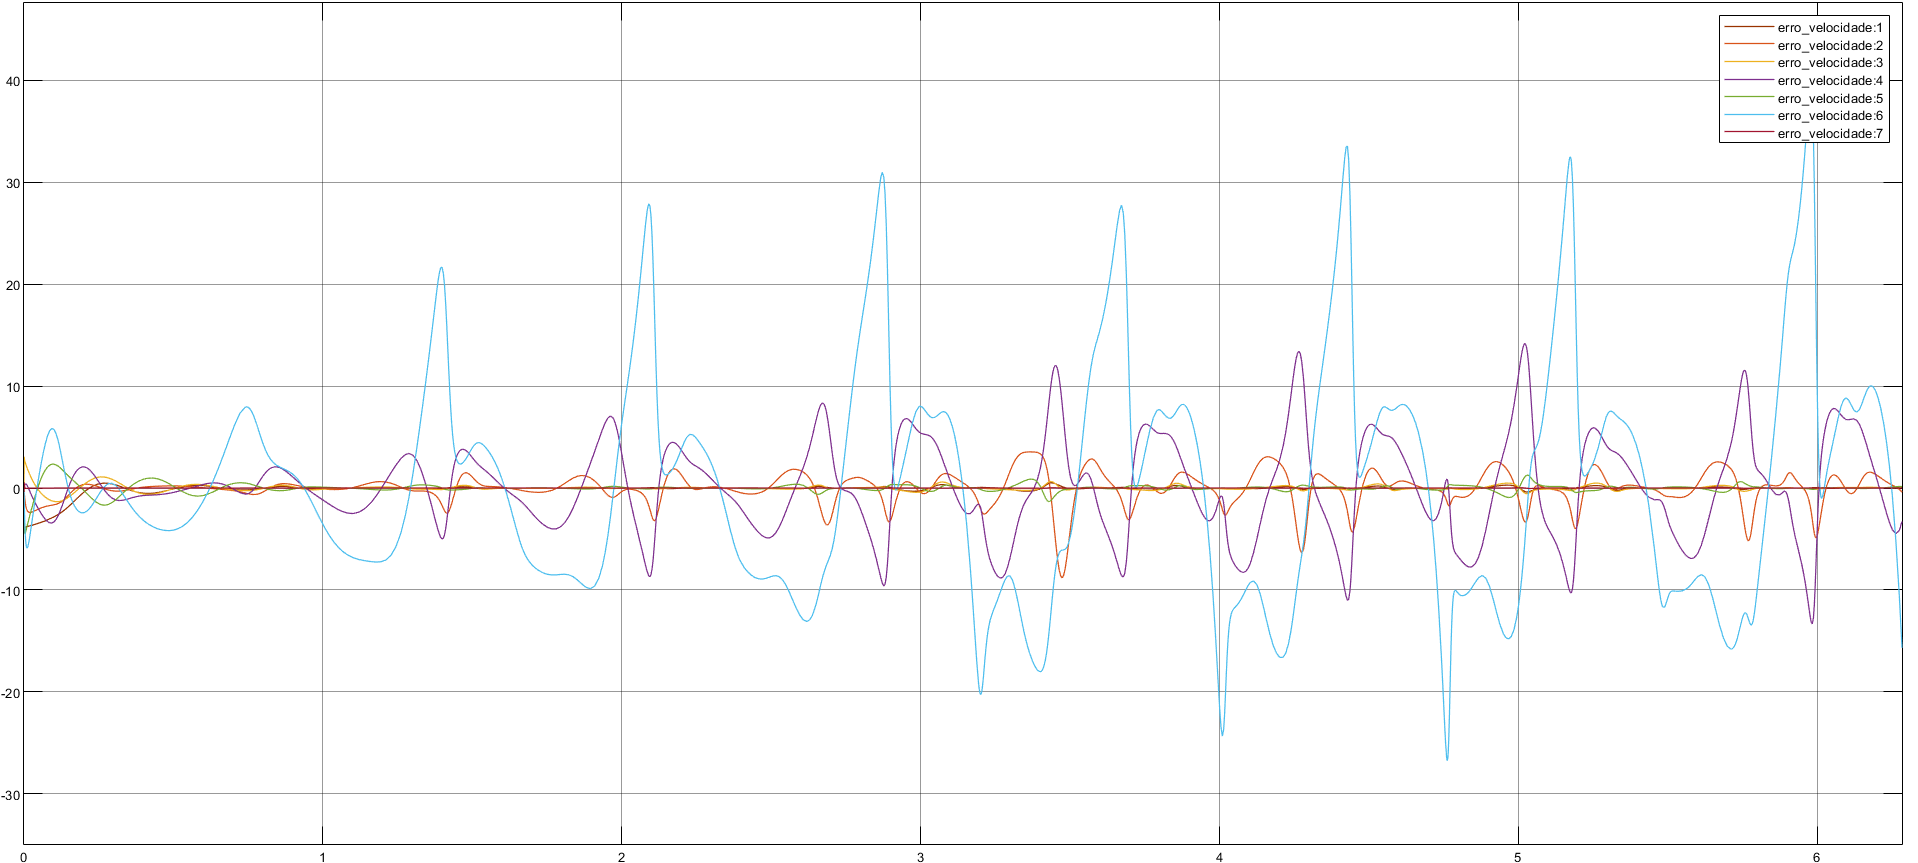
\includegraphics[width=\linewidth]{erro_velocidade_ppi_pi2_m.png}
        \caption{Erros de velocidades das juntas}
        \label{fig:erro_velocidade_ppi_pi2_m}
    \end{subfigure}%
    \caption{Controlador P-PI com massa adicional ($\omega_n = \pi/2$)}
    \label{fig:imagens_ppi_pi2_m}
\end{figure}

\subsection{Controlador por Torque Computado + PD}

É possível cancelar as não linearidades ao utilizar o torque computado (linearização por realimentação):

\begin{equation}
    \tau = M(\theta) [\ddot{\theta}_d + u] + C(\theta, \dot{\theta}) \dot{\theta} + G(\theta),
\end{equation}
obtém-se o sistema em malha fechada com o erro definido como \(\tilde{\theta} = \theta - \theta_d\):

\begin{equation}
    \ddot{\tilde{\theta}} = u.
\end{equation}
Ao se utilizar o controlador PD $(u = -K_p \tilde{\theta} - K_d \dot{\tilde{\theta}})$ no sistema acima, o erro do sistema é dado por:

\begin{equation}
    \ddot{\tilde{\theta}} + K_d \dot{\tilde{\theta}} + K_p \tilde{\theta} = 0.
\end{equation}
em que $K_d = 20$ e $K_p = 100$ para respeitar as especificações do projeto.

A seguir temos o diagrama do controlador por Torque Computado + PD implementado no Simulink:

\newpage

\begin{figure}[h]
    \centering
    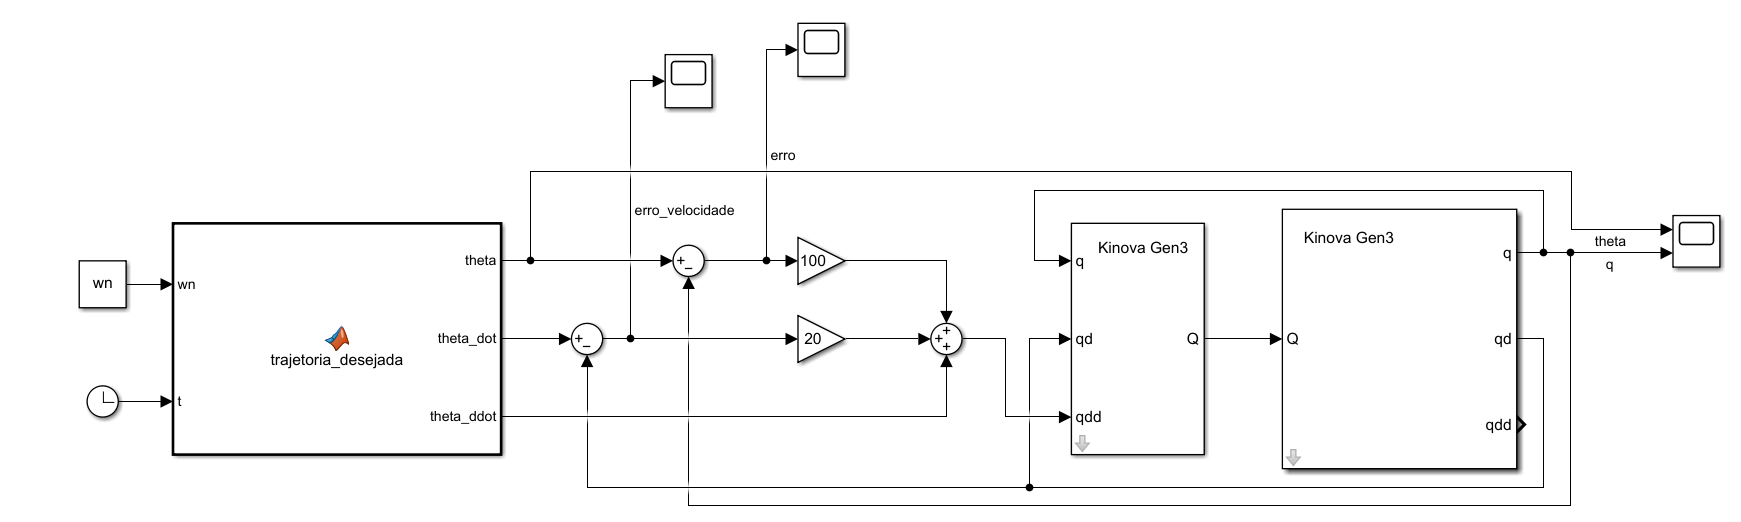
\includegraphics[scale=0.45]{diagrama_torque_computado_pd.png}
    \caption{Diagrama do controlador por Torque Computado + PD}
\end{figure}

Além disso, foi avaliado esse controlador para um intervalo de $2\pi$ segundos com um $\omega_n = \pi$.
Isso foi feito observando as posições das juntas,
o erro entre as posições das juntas e as posições das trajetórias desejadas e
o erro entre as velocidades das juntas e as velocidades das trajetórias desejadas.
A seguir temos os gráficos:

\begin{figure}[h!]
    \centering
    \begin{subfigure}[b]{0.49\textwidth}
        \centering
        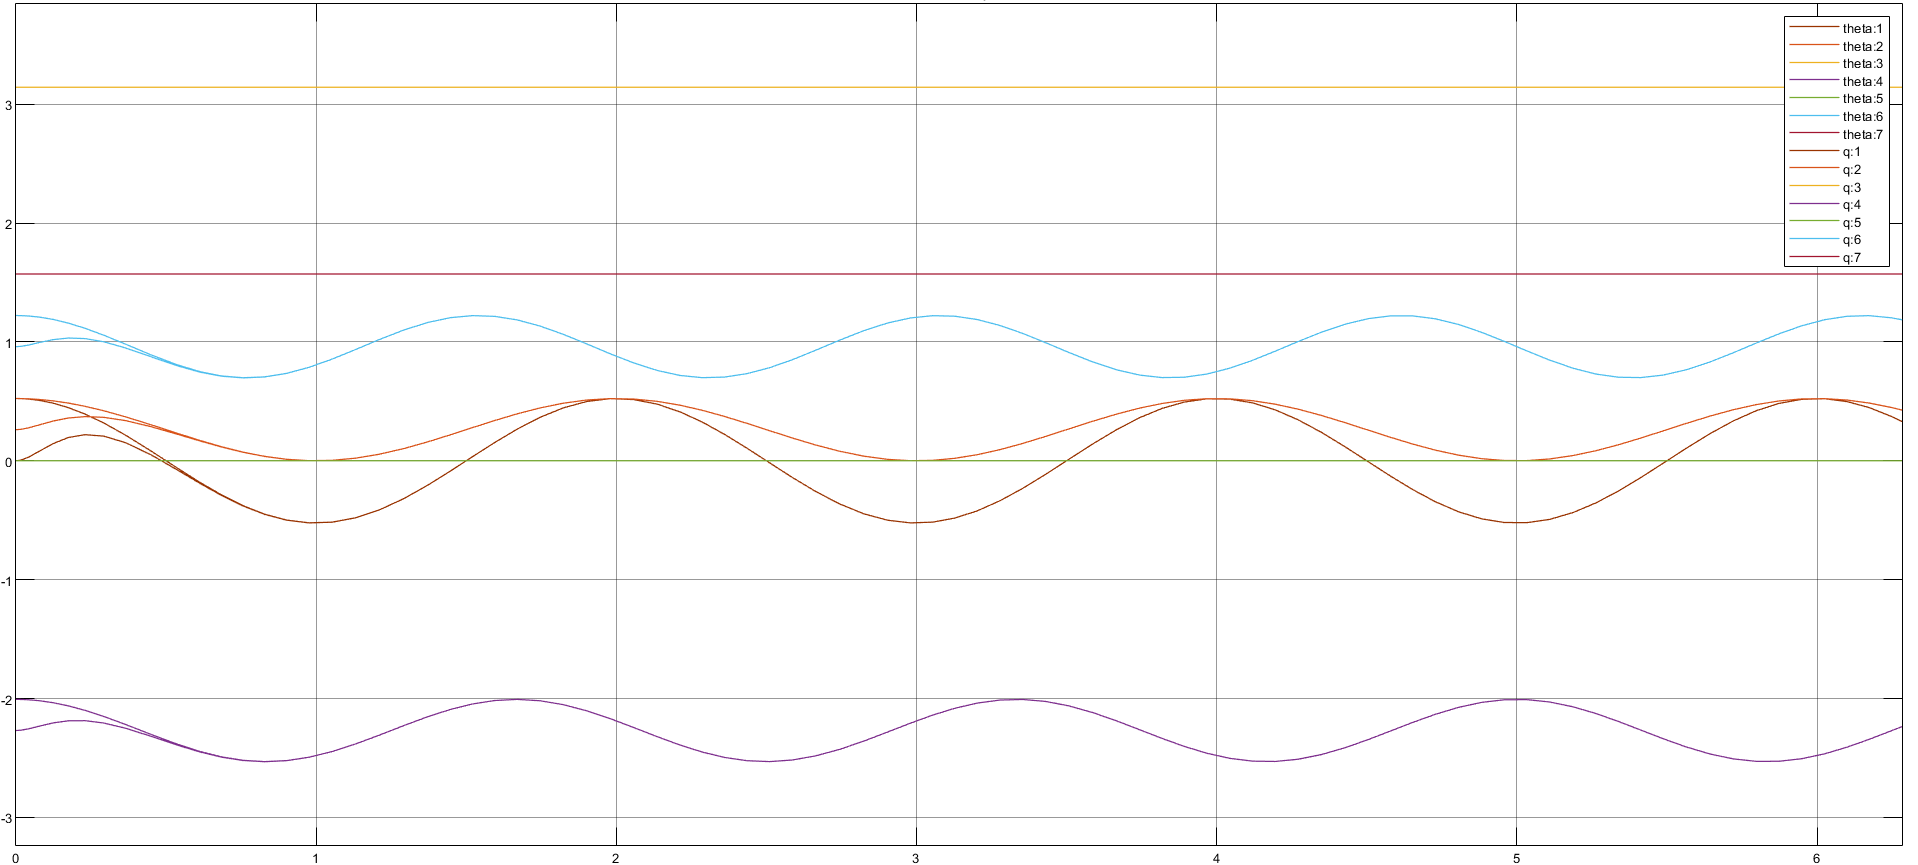
\includegraphics[width=\linewidth]{posicao_torque_computado_pd_pi.png}
        \caption{Posições das juntas}
        \label{fig:posicao_torque_computado_pd_pi}
    \end{subfigure}%
    \hfill
    \begin{subfigure}[b]{0.49\textwidth}
        \centering
        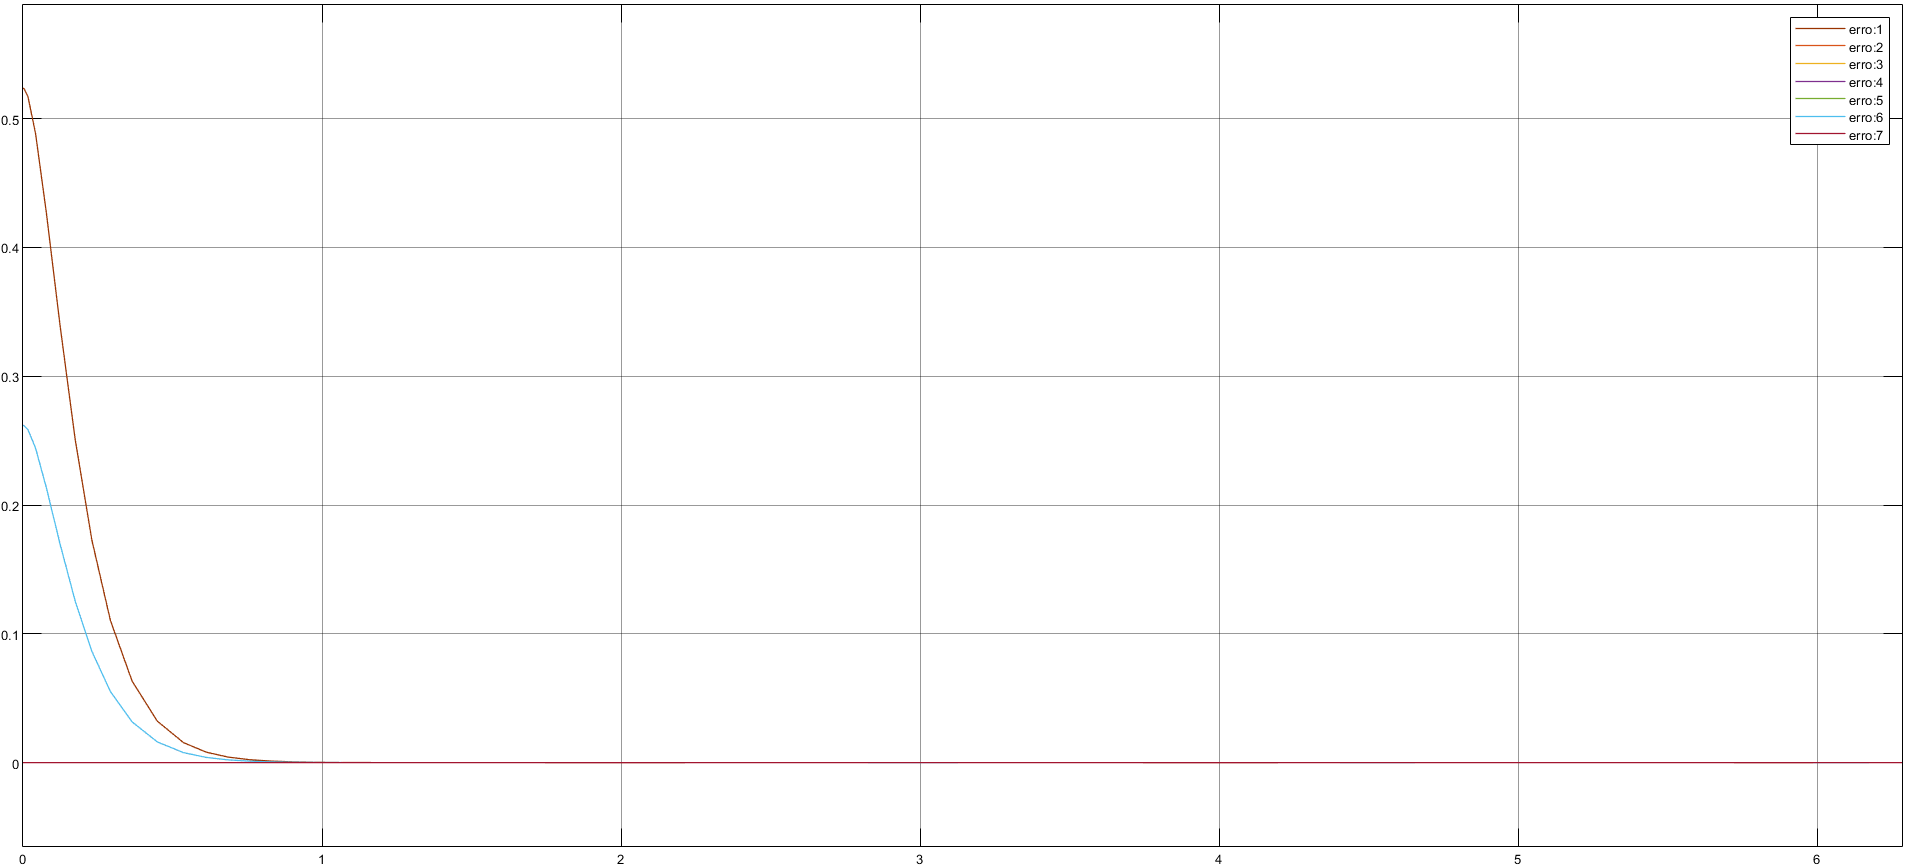
\includegraphics[width=\linewidth]{erro_torque_computado_pd_pi.png}
        \caption{Erros de posições das juntas}
        \label{fig:erro_torque_computado_pd_pi}
    \end{subfigure}%
    \hfill
    \begin{subfigure}[b]{0.49\textwidth}
        \centering
        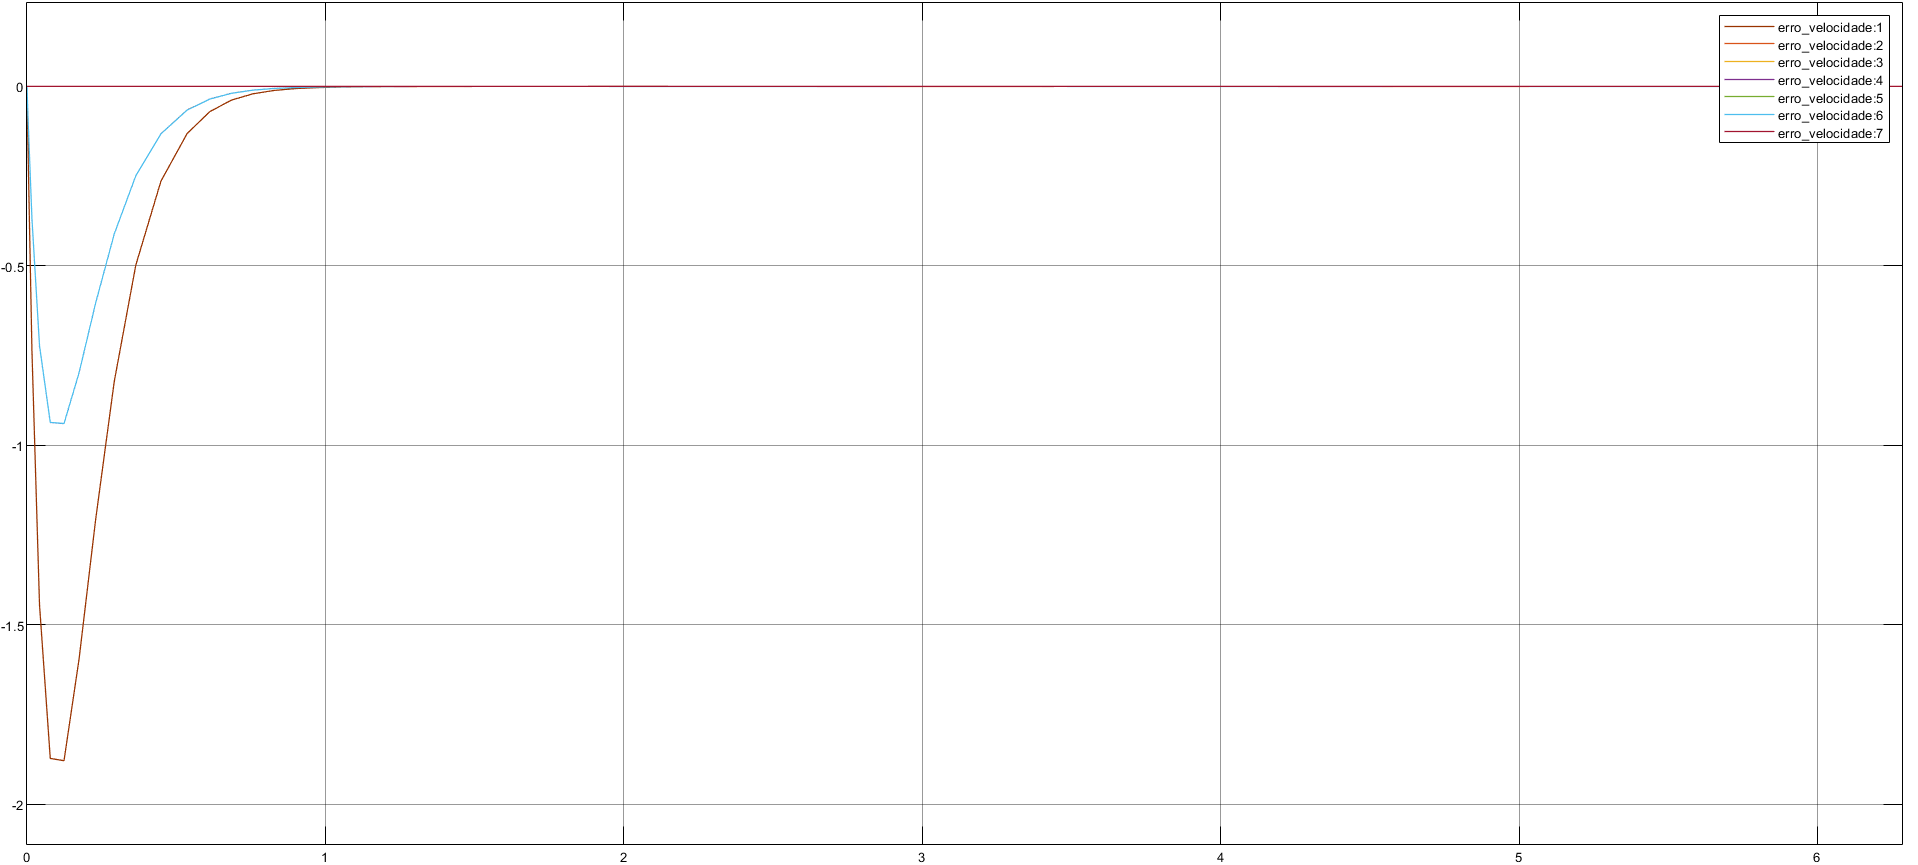
\includegraphics[width=\linewidth]{erro_velocidade_torque_computado_pd_pi.png}
        \caption{Erros de velocidades das juntas}
        \label{fig:erro_velocidade_torque_computado_pd_pi}
    \end{subfigure}%
    \caption{Controlador por Torque Computado + PD ($\omega_n = \pi$)}
    \label{fig:imagens_torque_computado_pd_pi}
\end{figure}

Isso também foi feito para $\omega_n = \pi/2$. Obtendo os seguintes resultados:

\newpage

\begin{figure}[h!]
    \centering
    \begin{subfigure}[b]{0.49\textwidth}
        \centering
        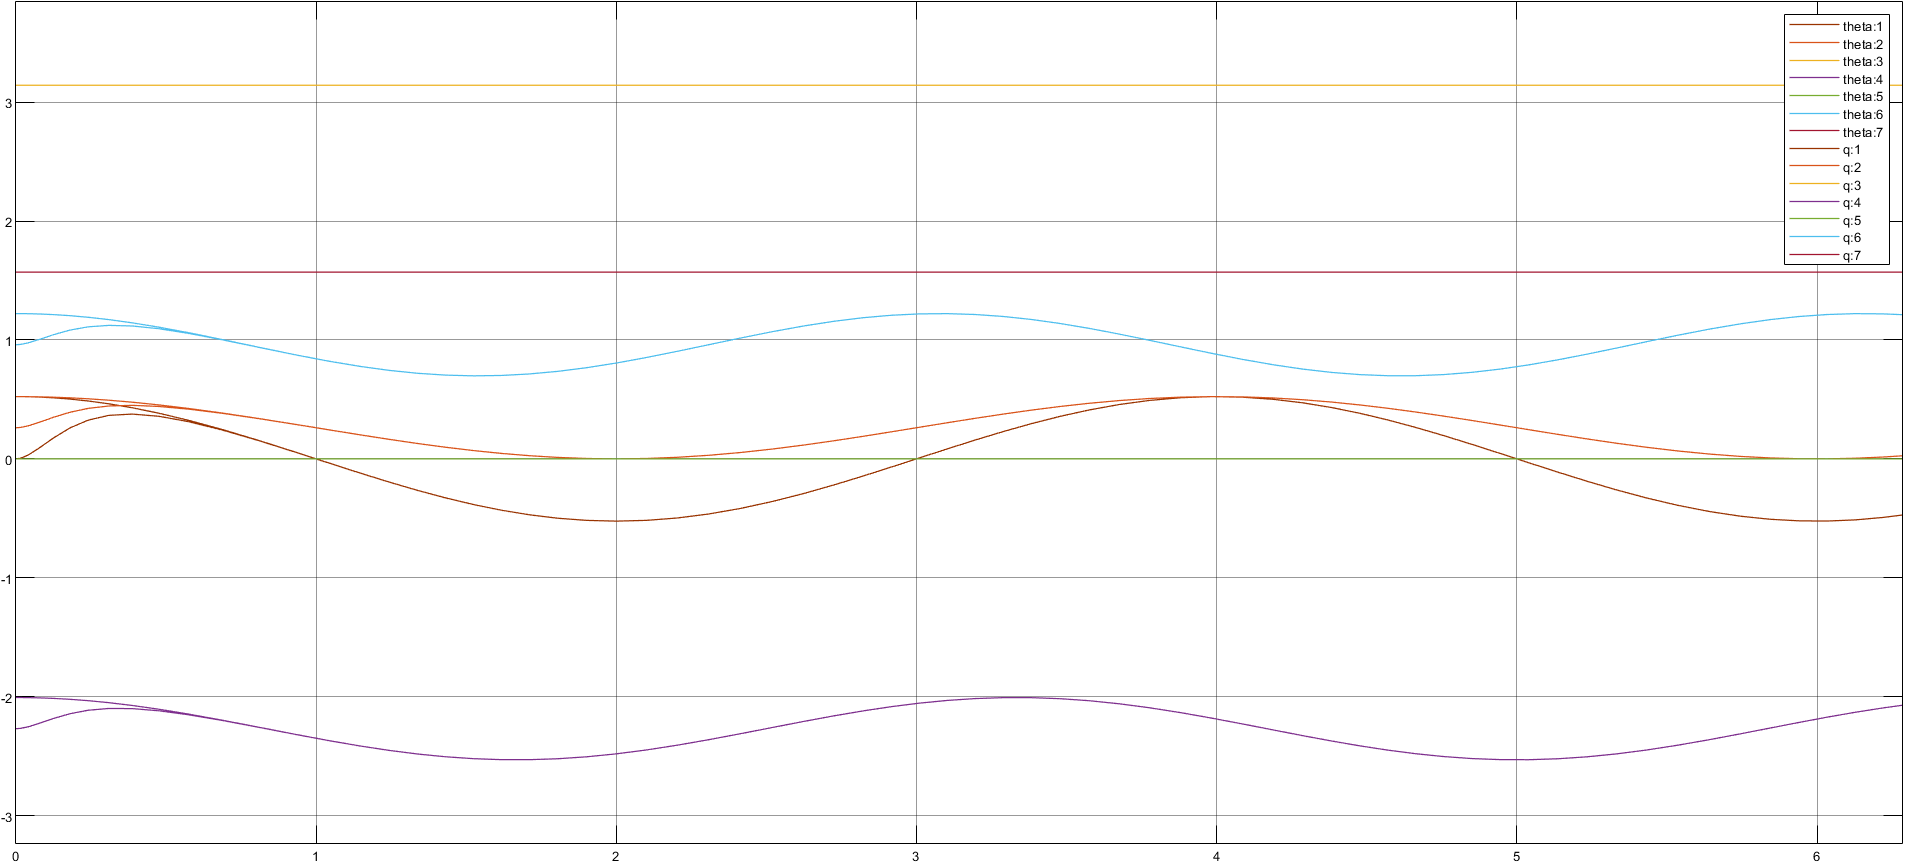
\includegraphics[width=\linewidth]{posicao_torque_computado_pd_pi2.png}
        \caption{Posições das juntas}
        \label{fig:posicao_torque_computado_pd_pi2}
    \end{subfigure}%
    \hfill
    \begin{subfigure}[b]{0.49\textwidth}
        \centering
        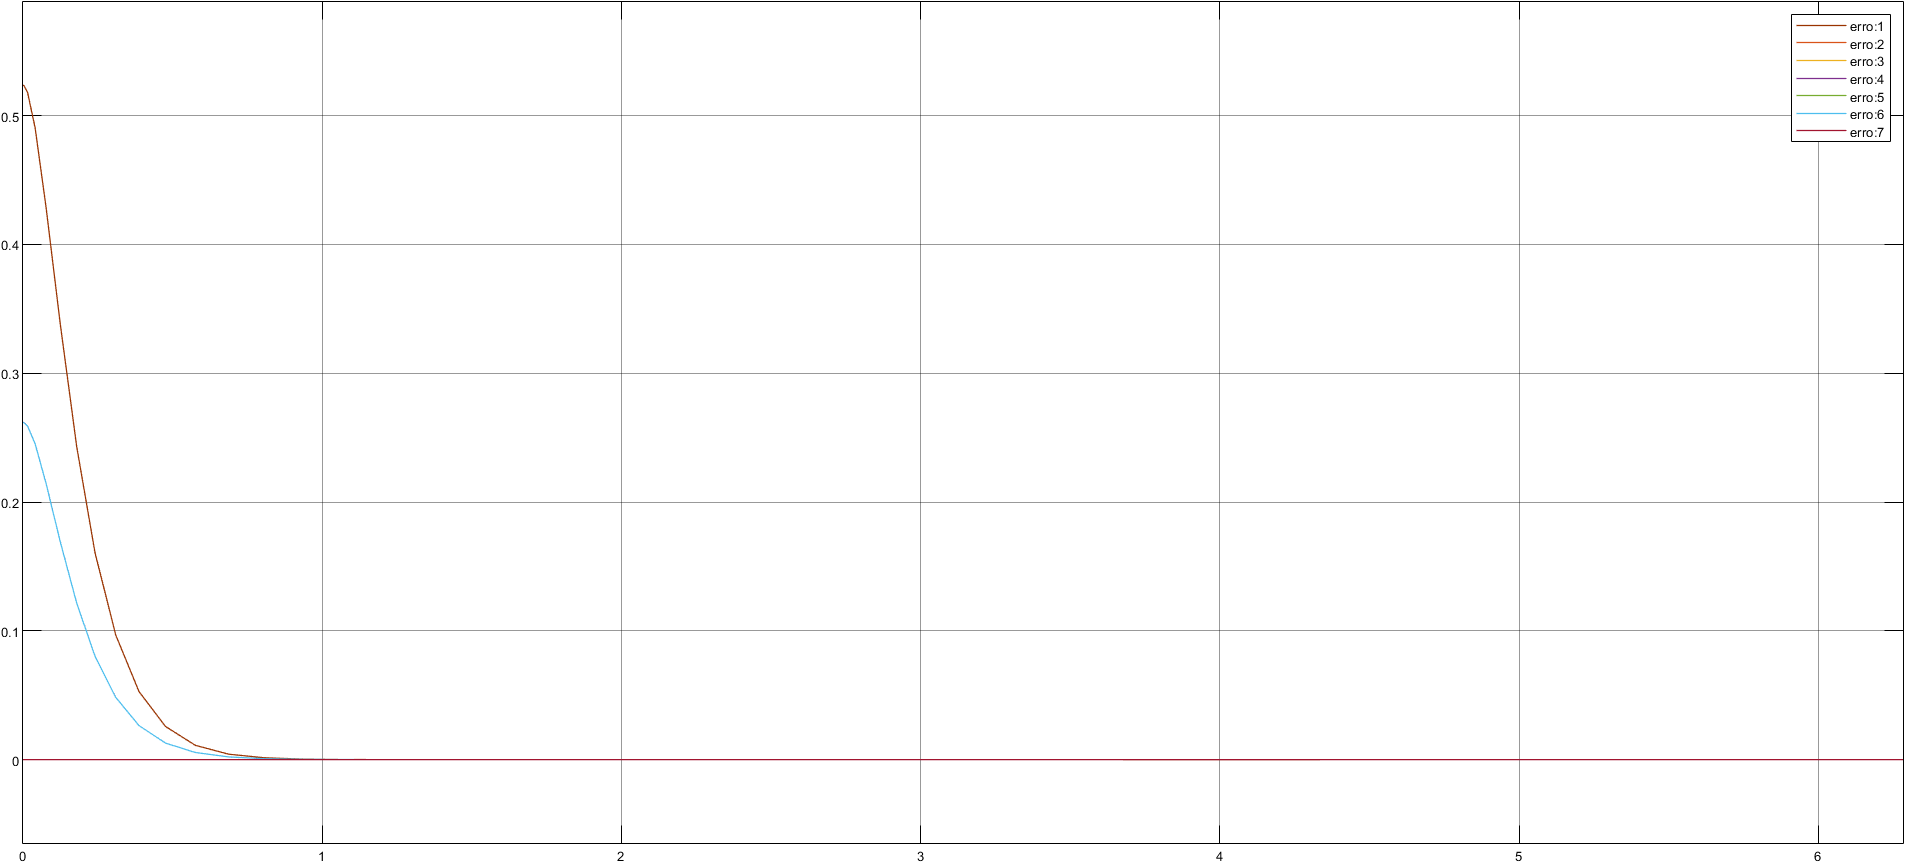
\includegraphics[width=\linewidth]{erro_torque_computado_pd_pi2.png}
        \caption{Erros de posições das juntas}
        \label{fig:erro_torque_computado_pd_pi2}
    \end{subfigure}%
    \hfill
    \begin{subfigure}[b]{0.49\textwidth}
        \centering
        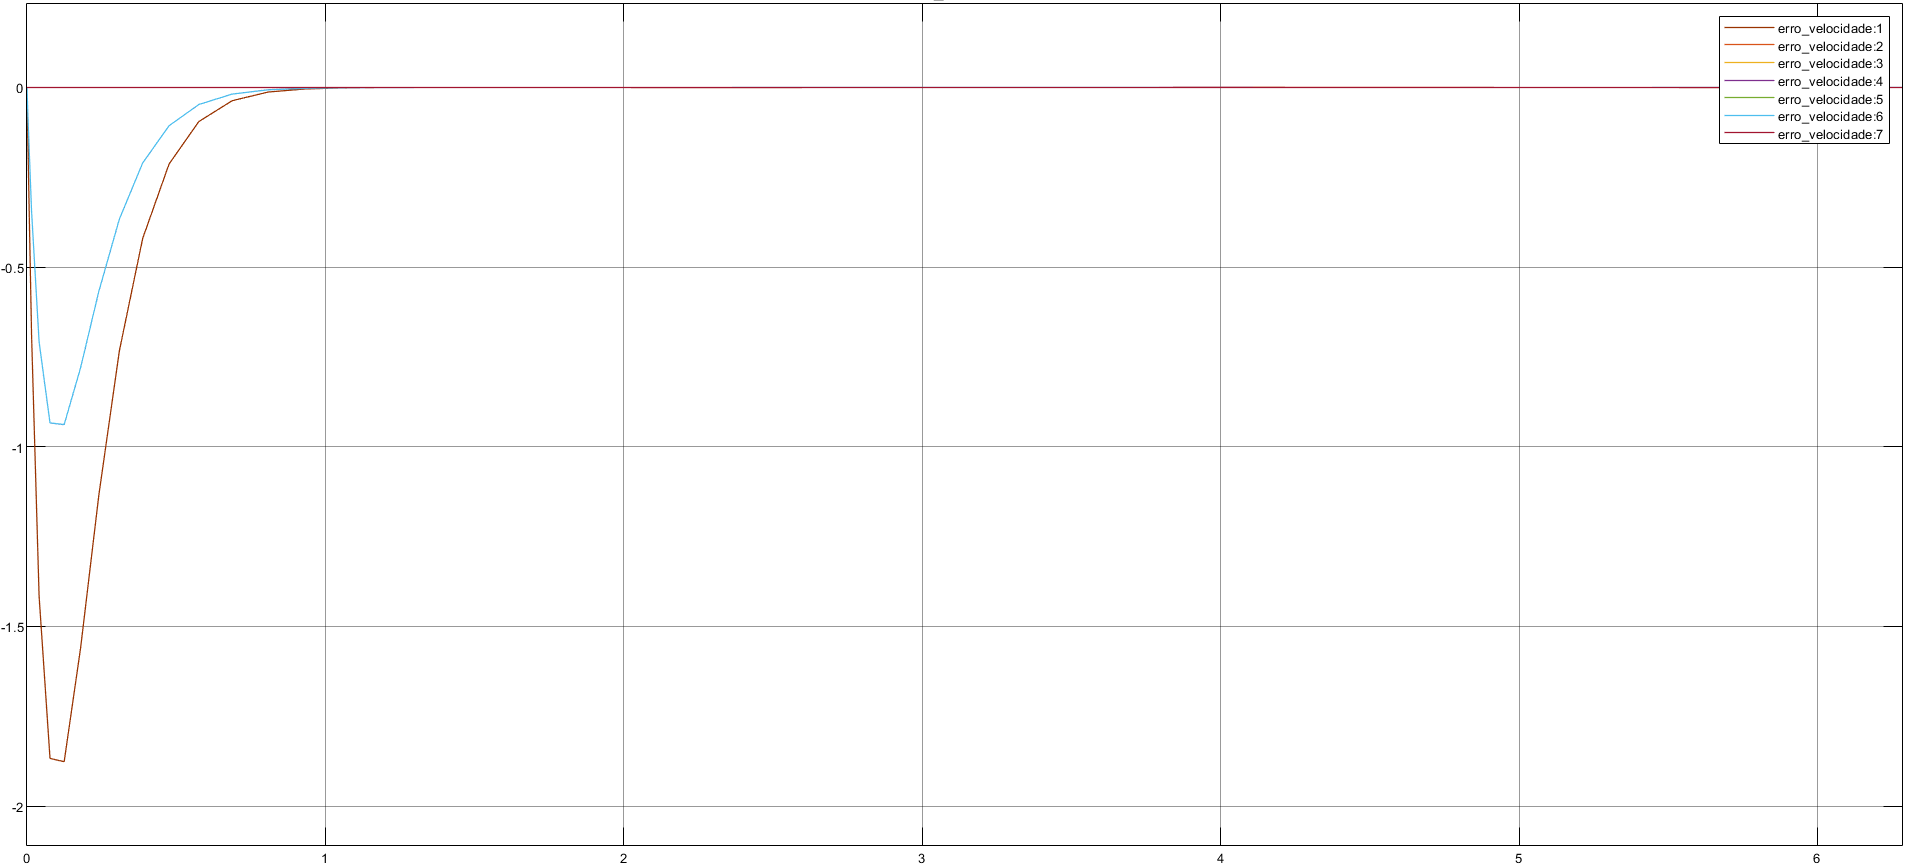
\includegraphics[width=\linewidth]{erro_velocidade_torque_computado_pd_pi2.png}
        \caption{Erros de velocidades das juntas}
        \label{fig:erro_velocidade_torque_computado_pd_pi2}
    \end{subfigure}%
    \caption{Controlador por Torque Computado + PD ($\omega_n = \pi/2$)}
    \label{fig:imagens_torque_computado_pd_pi2}
\end{figure}

Além disso, foi feito a simulação com a massa adicional de 10kg para $\omega_n = \pi$:

\begin{figure}[h!]
    \centering
    \begin{subfigure}[b]{0.49\textwidth}
        \centering
        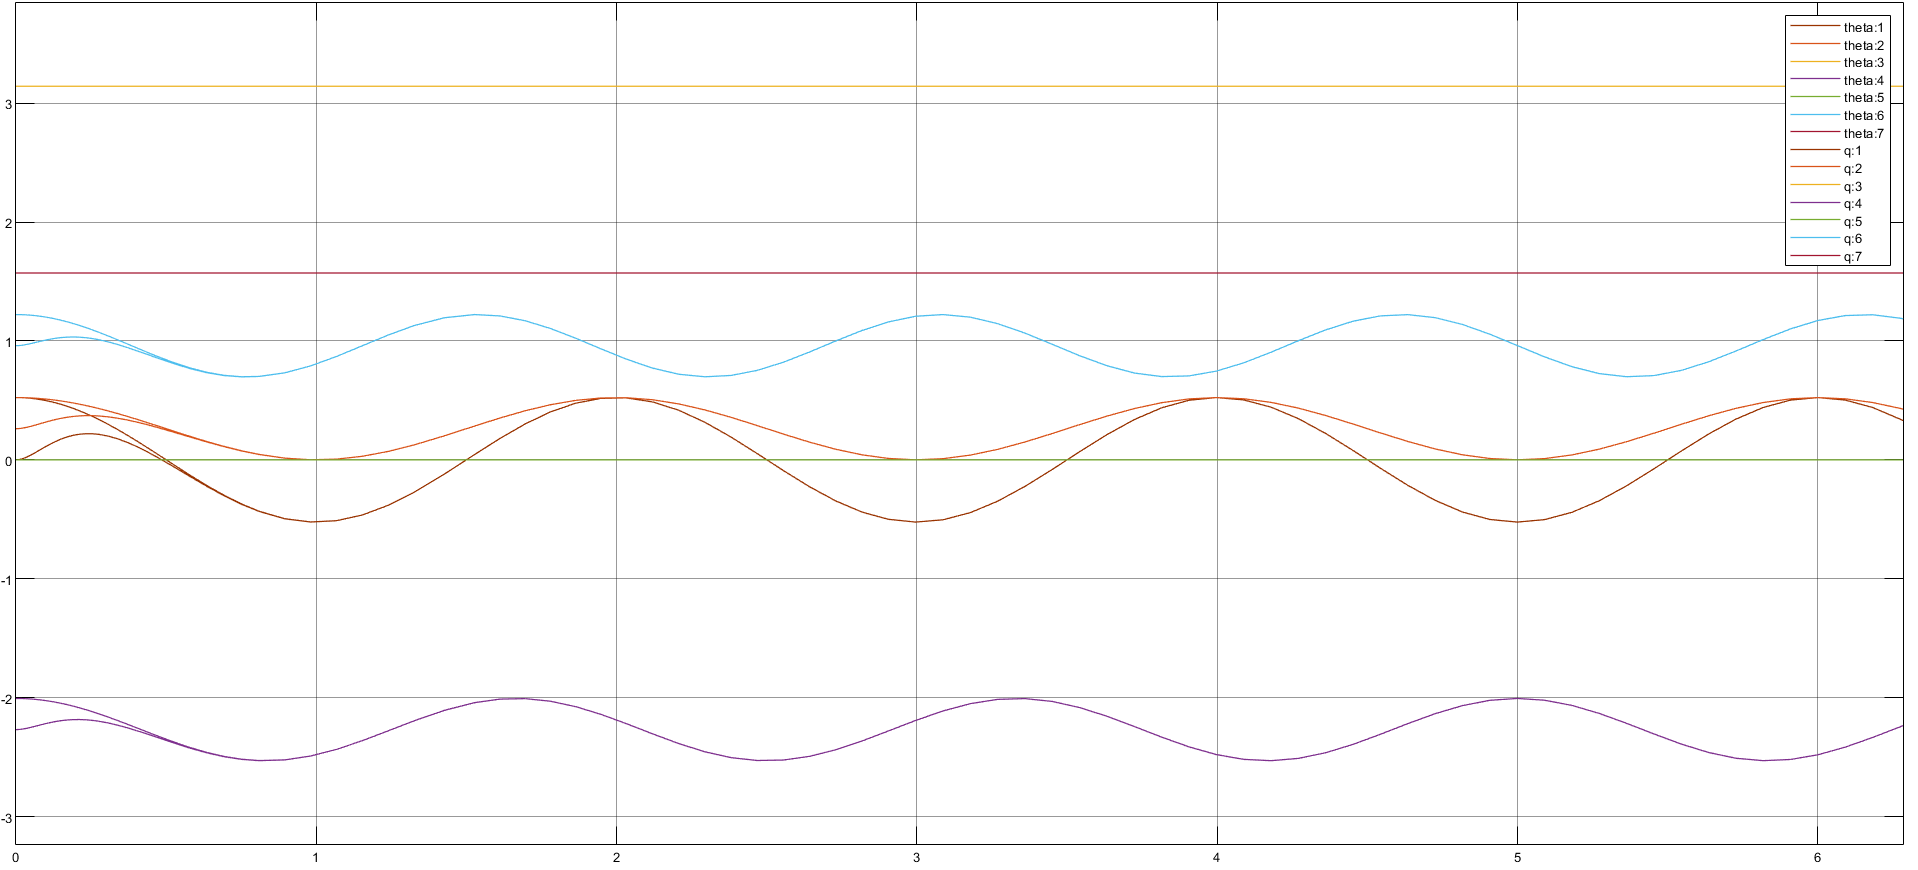
\includegraphics[width=\linewidth]{posicao_torque_computado_pd_pi_m.png}
        \caption{Posições das juntas}
        \label{fig:posicao_torque_computado_pd_pi_m}
    \end{subfigure}%
    \hfill
    \begin{subfigure}[b]{0.49\textwidth}
        \centering
        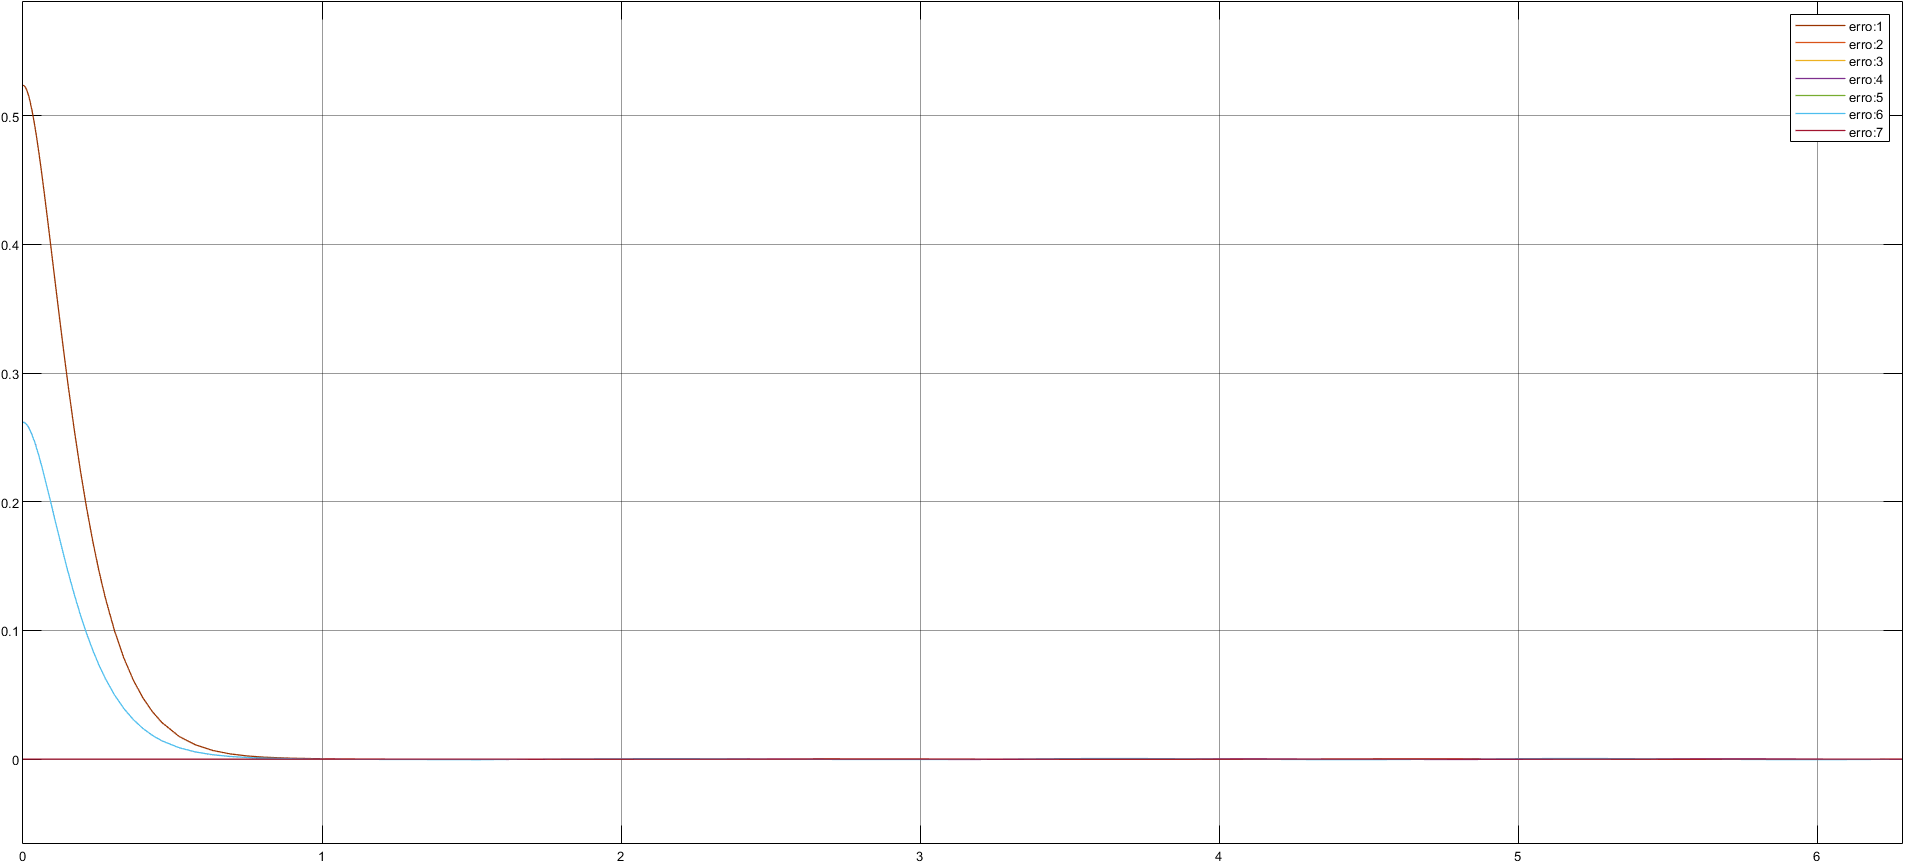
\includegraphics[width=\linewidth]{erro_torque_computado_pd_pi_m.png}
        \caption{Erros de posições das juntas}
        \label{fig:erro_torque_computado_pd_pi_m}
    \end{subfigure}%
    \hfill
    \begin{subfigure}[b]{0.49\textwidth}
        \centering
        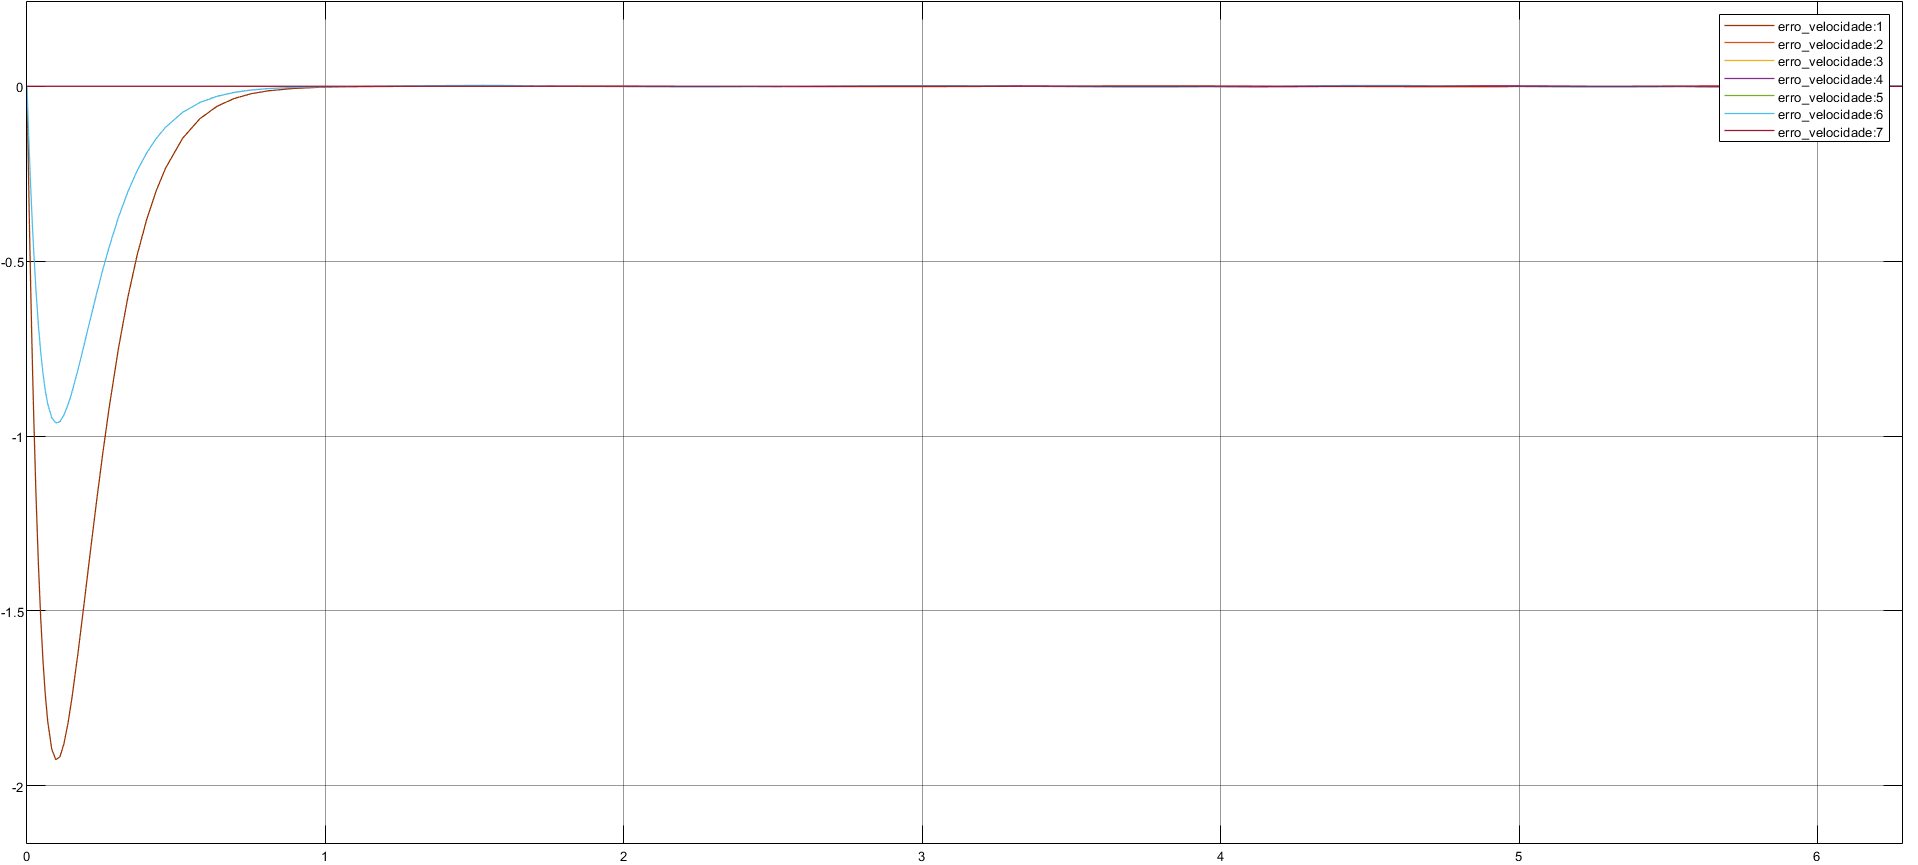
\includegraphics[width=\linewidth]{erro_velocidade_torque_computado_pd_pi_m.png}
        \caption{Erros de velocidades das juntas}
        \label{fig:erro_velocidade_torque_computado_pd_pi_m}
    \end{subfigure}%
    \caption{Controlador por Torque Computado + PD ($\omega_n = \pi$)}
    \label{fig:imagens_torque_computado_pd_pi_m}
\end{figure}

Ademais, foi feito a simulação com a massa adicional de 10kg para $\omega_n = \pi/2$:

\begin{figure}[h!]
    \centering
    \begin{subfigure}[b]{0.49\textwidth}
        \centering
        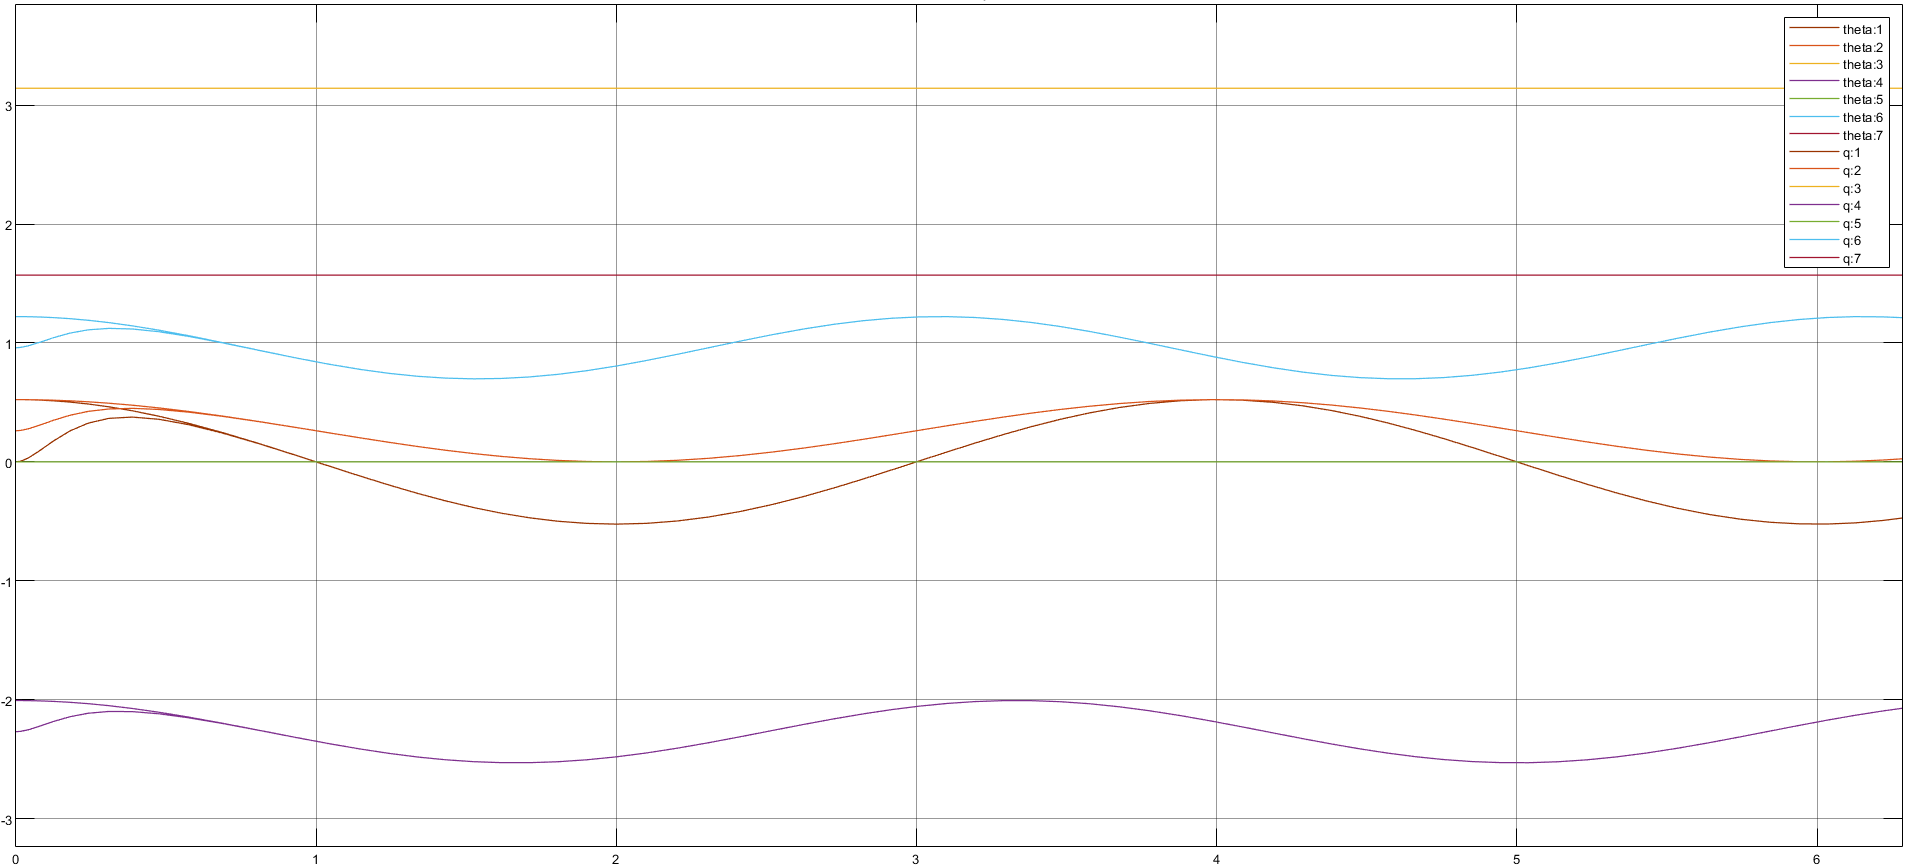
\includegraphics[width=\linewidth]{posicao_torque_computado_pd_pi2_m.png}
        \caption{Posições das juntas}
        \label{fig:posicao_torque_computado_pd_pi2_m}
    \end{subfigure}%
    \hfill
    \begin{subfigure}[b]{0.49\textwidth}
        \centering
        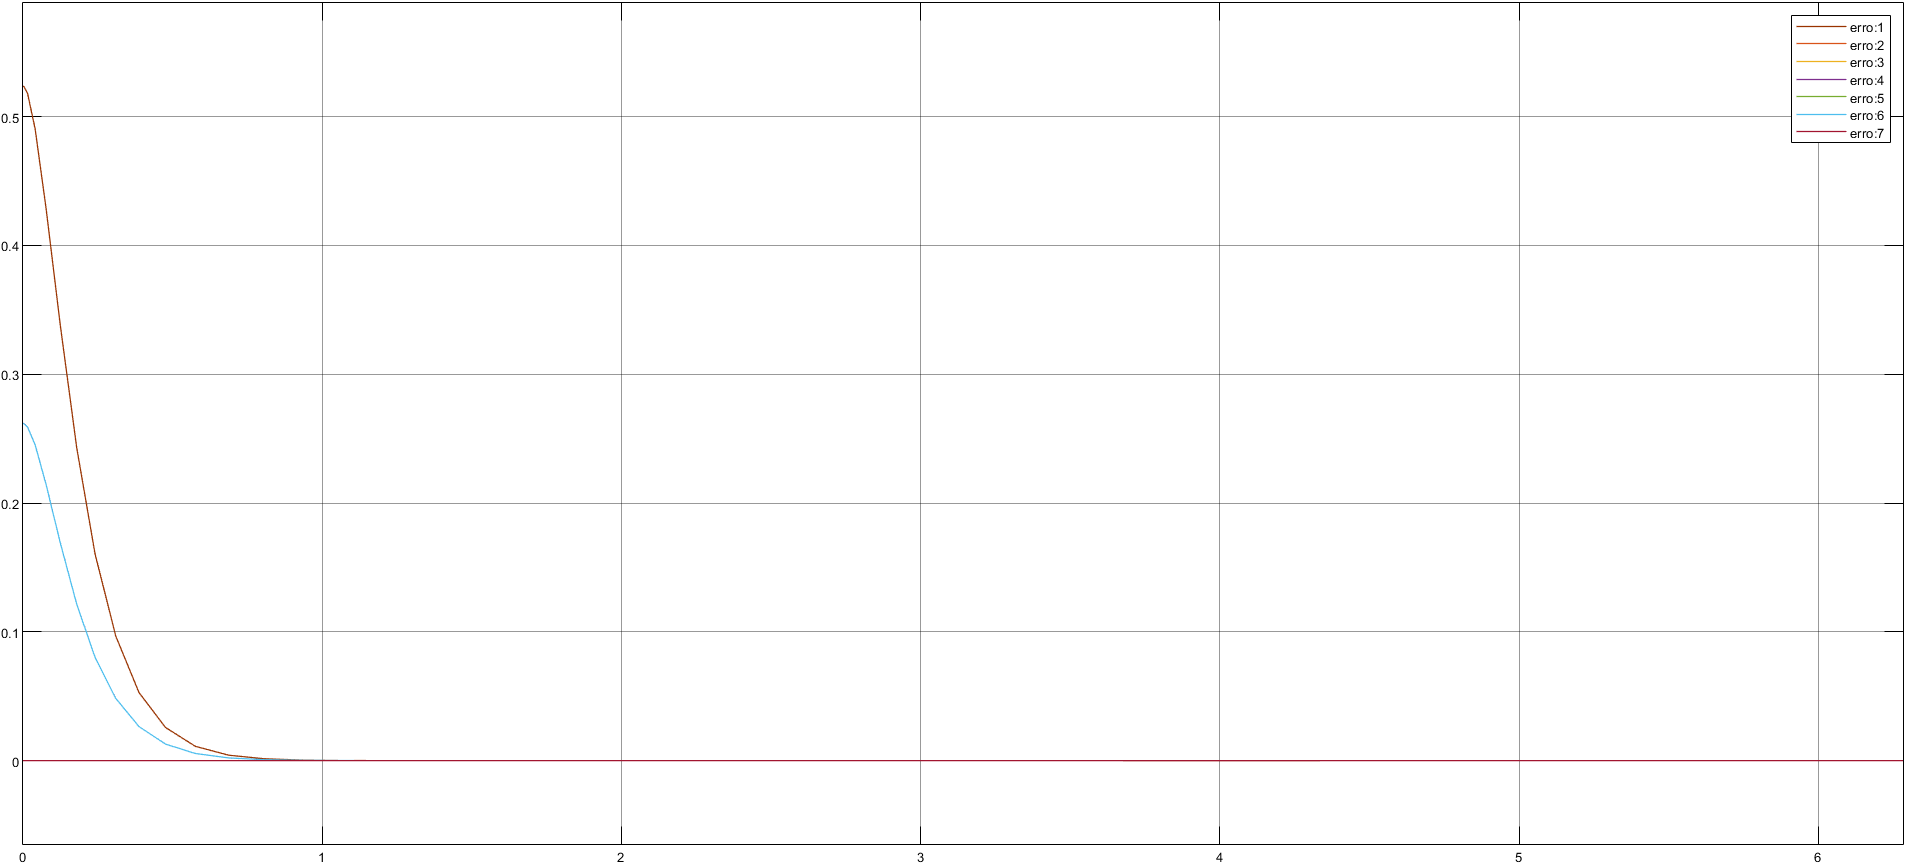
\includegraphics[width=\linewidth]{erro_torque_computado_pd_pi2_m.png}
        \caption{Erros de posições das juntas}
        \label{fig:erro_torque_computado_pd_pi2_m}
    \end{subfigure}%
    \hfill
    \begin{subfigure}[b]{0.49\textwidth}
        \centering
        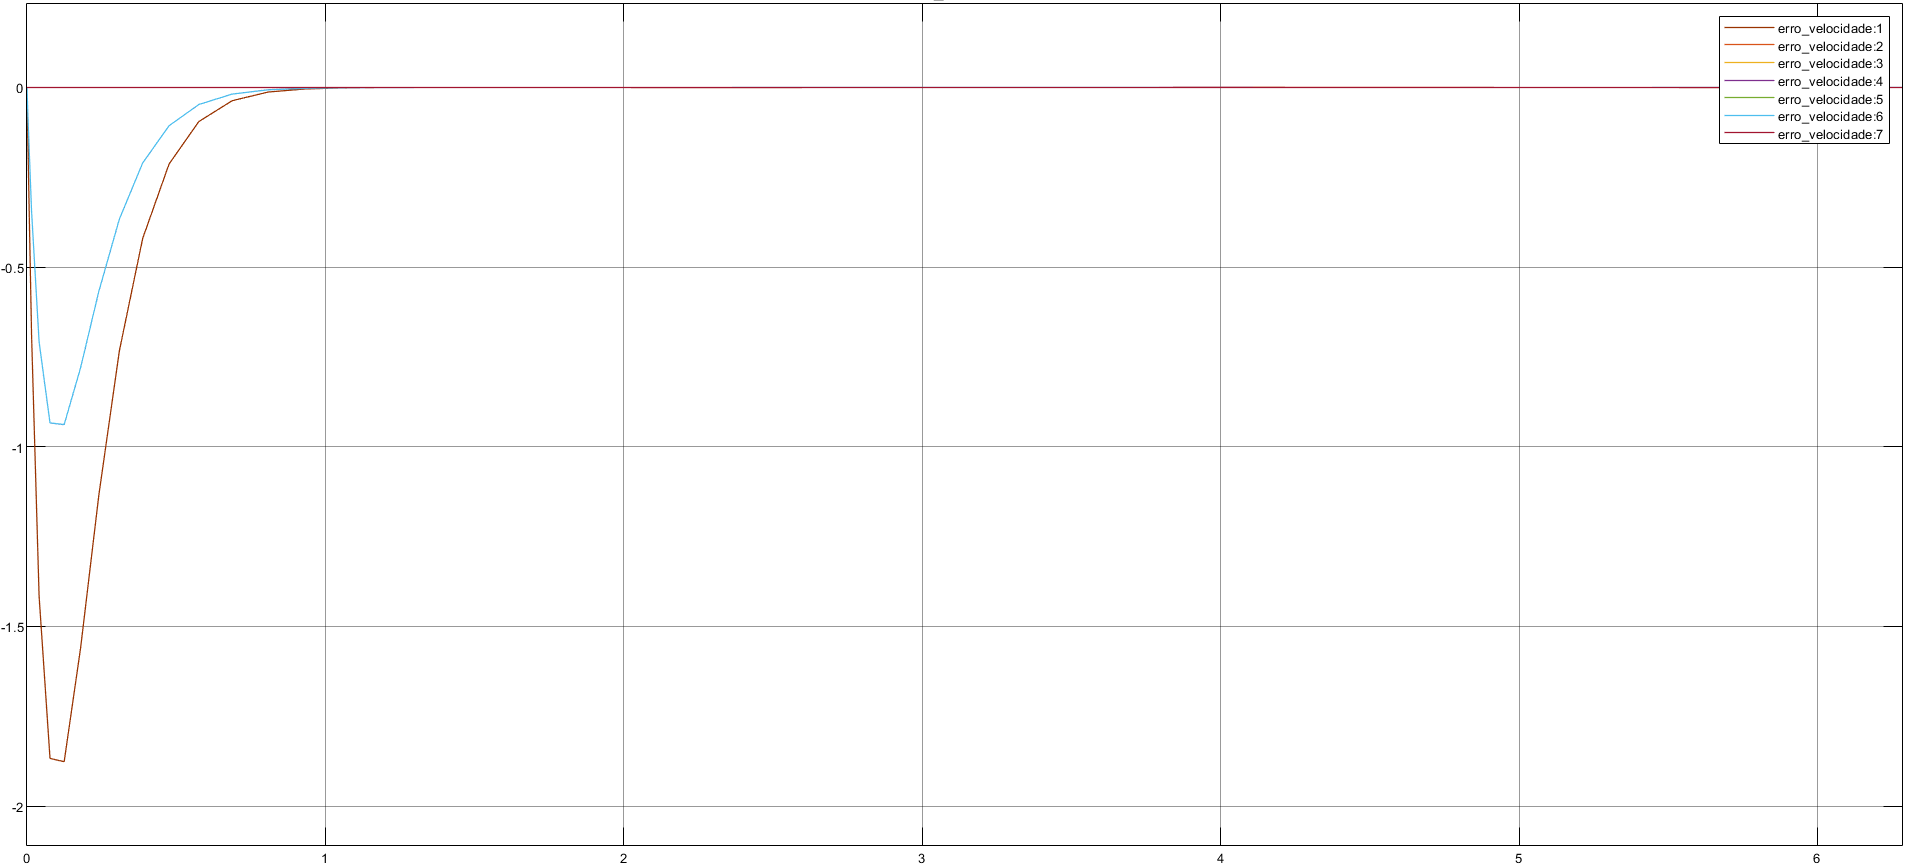
\includegraphics[width=\linewidth]{erro_velocidade_torque_computado_pd_pi2_m.png}
        \caption{Erros de velocidades das juntas}
        \label{fig:erro_velocidade_torque_computado_pd_pi2_m}
    \end{subfigure}%
    \caption{Controlador por Torque Computado + PD ($\omega_n = \pi/2$)}
    \label{fig:imagens_torque_computado_pd_pi2_m}
\end{figure}

\subsection{Controlador de Slotine \& Li}

Para validar o modelo de controle apresentado, foi realizado uma série de experimentos ajustando os parâmetros \( K_d \) e \( \Lambda \) com o objetivo de alcançar um desempenho próximo ao projetado.
Após diversas iterações, os valores \( K_d = 5 \) e \( \Lambda = 10 \) foram escolhidos,
pois proporcionaram uma resposta do sistema estável e adequada ao critério de desempenho definido.
A lei de controle utilizada foi implementada conforme descrito anteriormente, com \(\sigma\) sendo ajustada para minimizar o erro de rastreamento e garantir o cumprimento das especificações.
Os valores de \( K_d \) e \( \Lambda \) foram ajustados experimentalmente, buscando uma resposta dinâmica consistente com o comportamento projetado.
Obtendo o seguinte diagrama:

\begin{figure}[h]
    \centering
    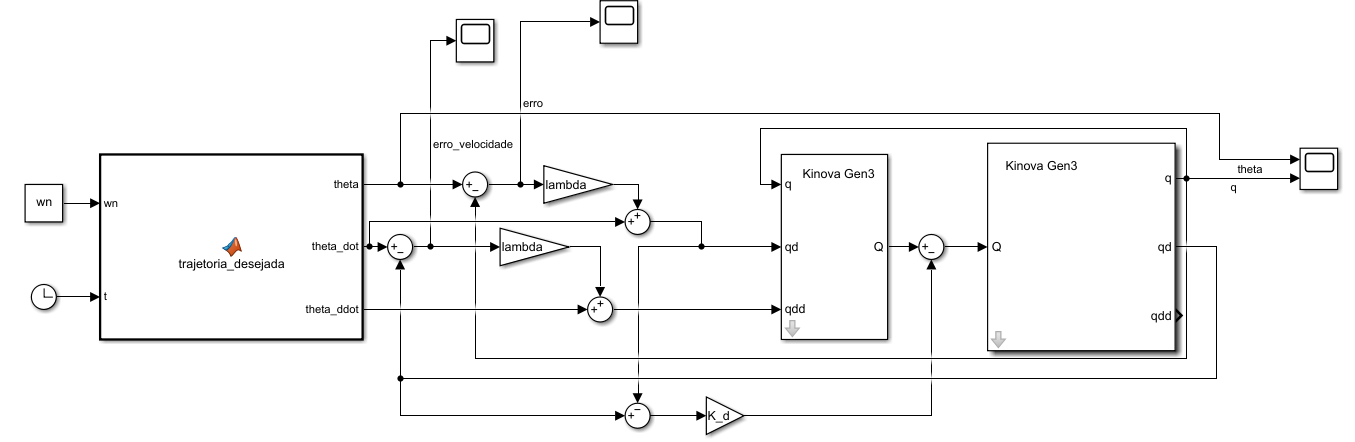
\includegraphics[scale=0.45]{diagrama_slotine_li.png}
    \caption{Diagrama do controlador de Slotine \& Li}
\end{figure}

Então, foi feita a simulação para $\omega_n = \pi$. Obtendo os seguintes resultados:

\begin{figure}[h!]
    \centering
    \begin{subfigure}[b]{0.49\textwidth}
        \centering
        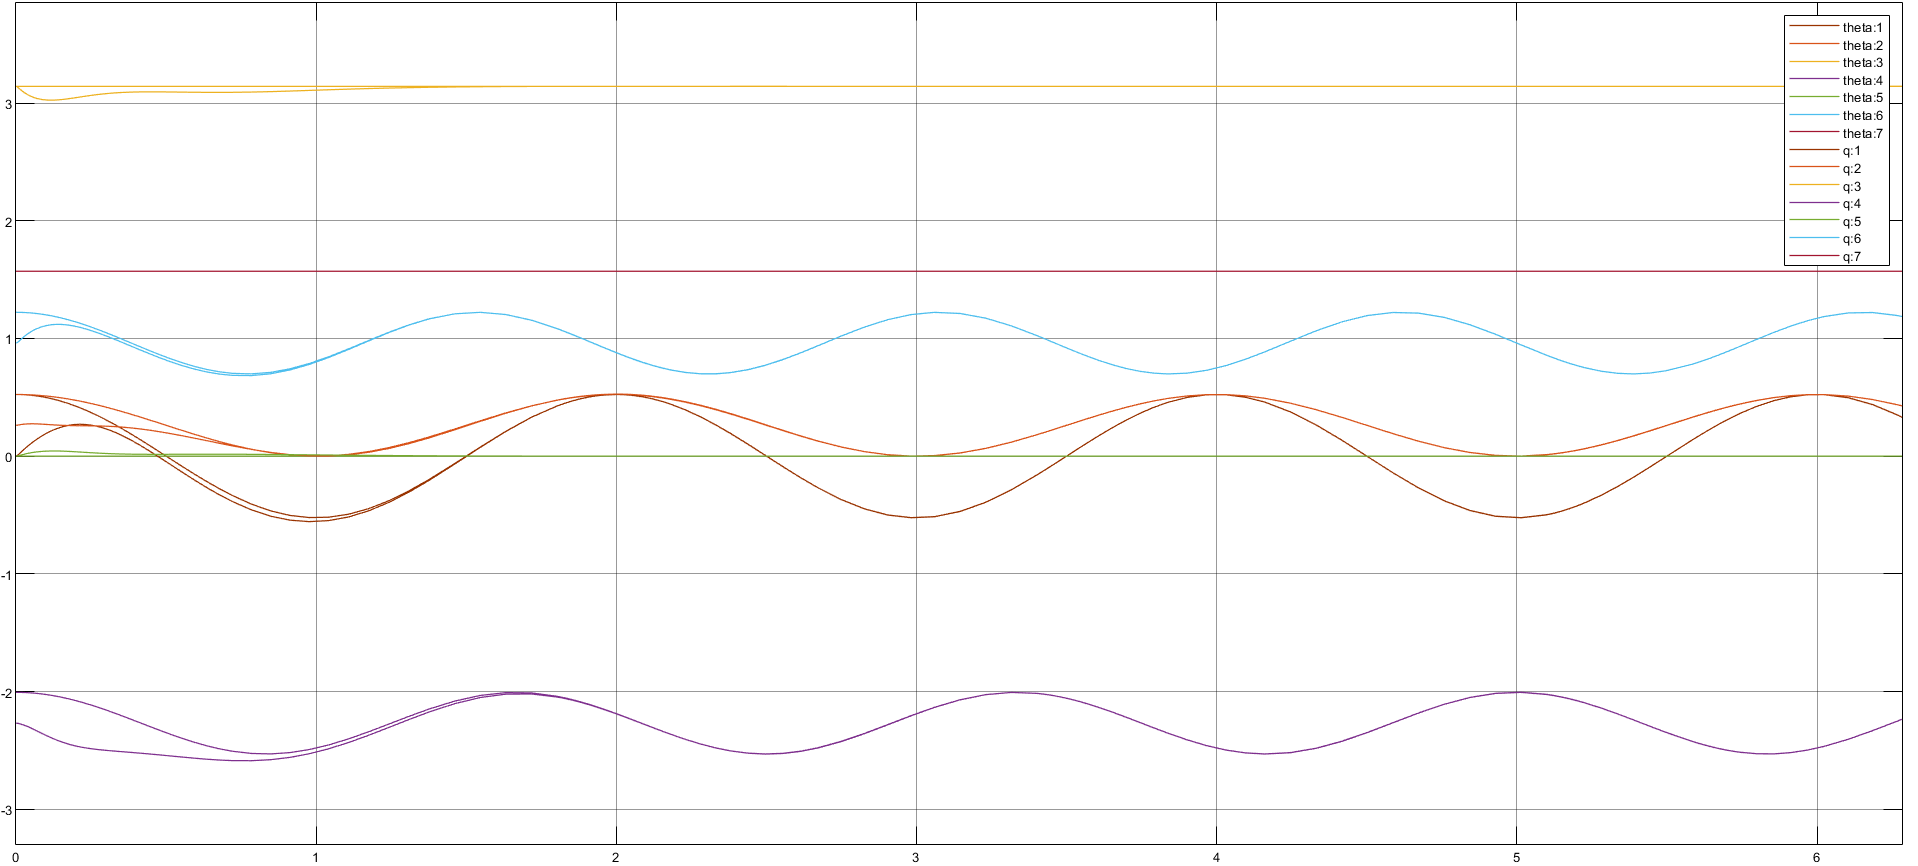
\includegraphics[width=\linewidth]{posicao_slotine_li_pi.png}
        \caption{Posições das juntas}
        \label{fig:posicao_slotine_li_pi}
    \end{subfigure}%
    \hfill
    \begin{subfigure}[b]{0.49\textwidth}
        \centering
        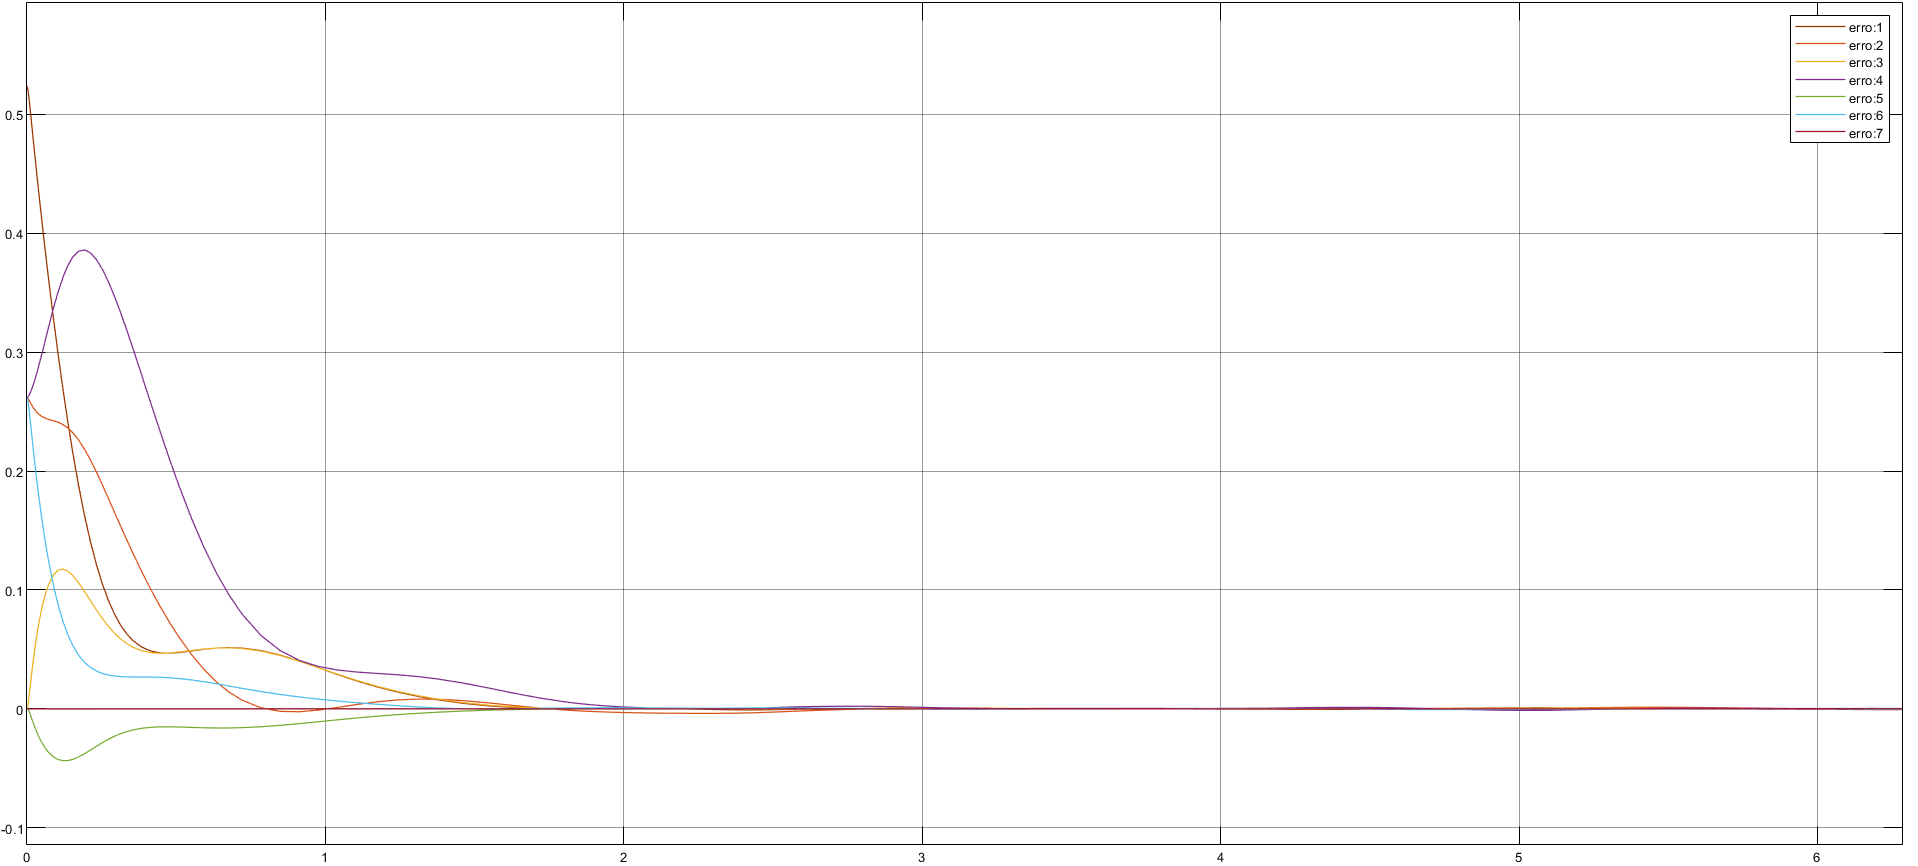
\includegraphics[width=\linewidth]{erro_slotine_li_pi.png}
        \caption{Erros de posições das juntas}
        \label{fig:erro_slotine_li_pi}
    \end{subfigure}%
    \hfill
    \begin{subfigure}[b]{0.49\textwidth}
        \centering
        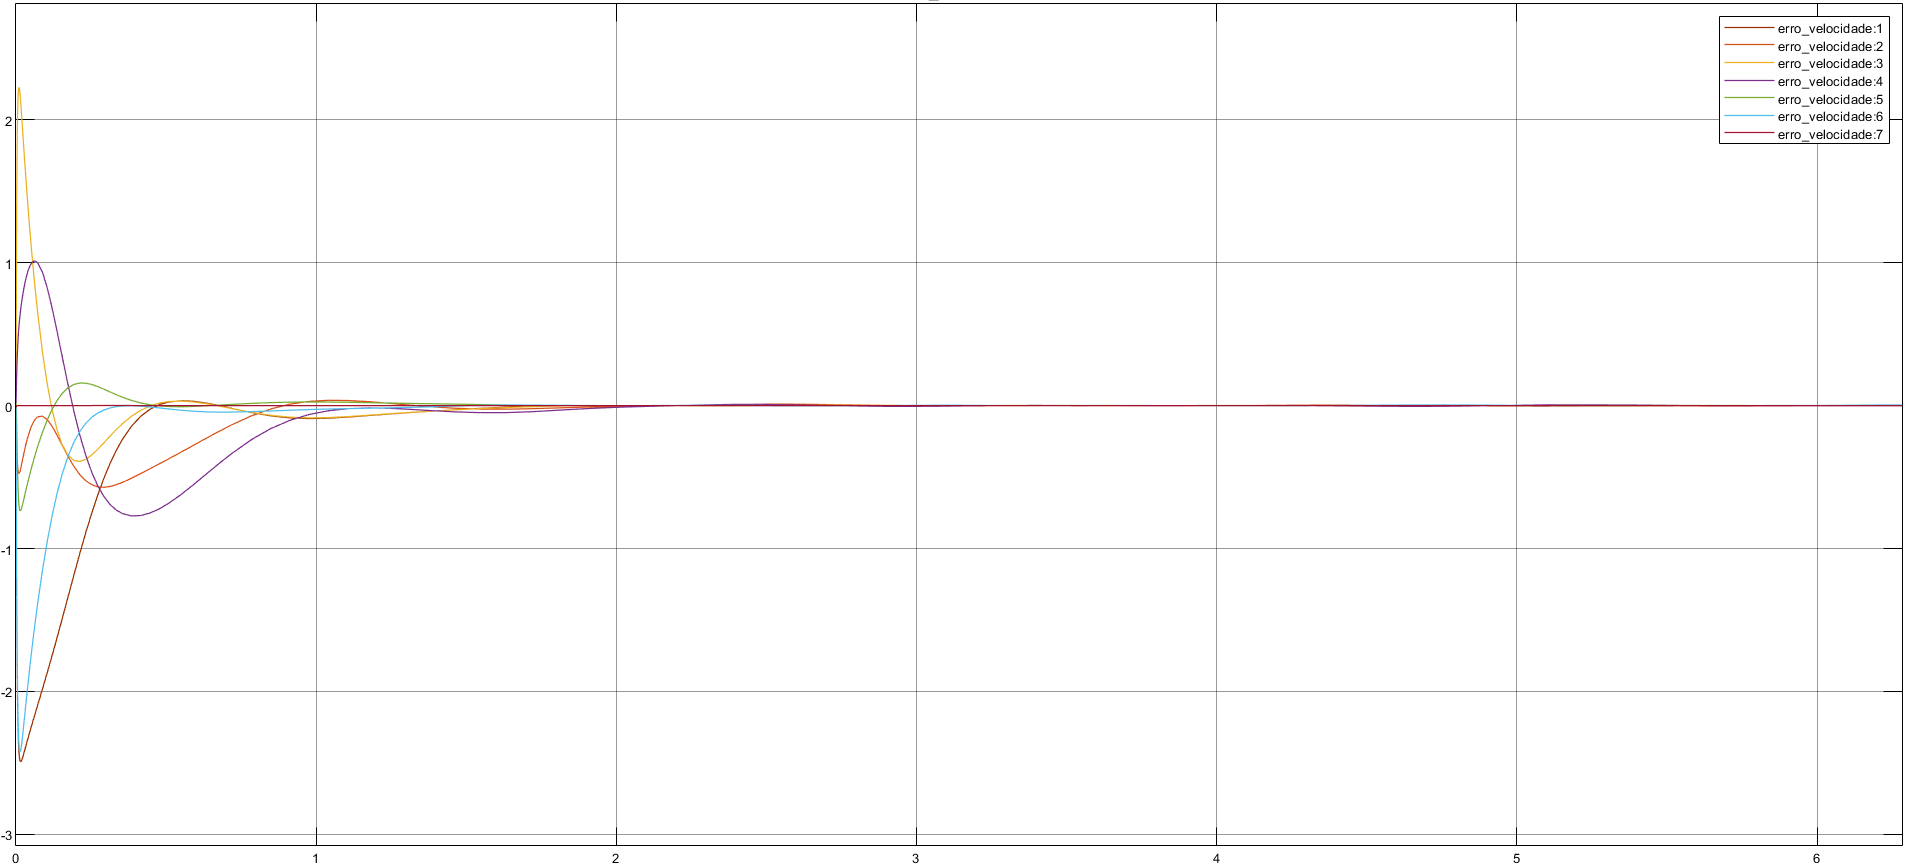
\includegraphics[width=\linewidth]{erro_velocidade_slotine_li_pi.png}
        \caption{Erros de velocidades das juntas}
        \label{fig:erro_velocidade_slotine_li_pi}
    \end{subfigure}%
    \caption{Controlador por Slotine \& Li ($\omega_n = \pi$)}
    \label{fig:imagens_slotine_li_pi}
\end{figure}

Isso também foi feito para $\omega_n = \pi/2$. Obtendo os seguintes resultados:

\begin{figure}[h!]
    \centering
    \begin{subfigure}[b]{0.49\textwidth}
        \centering
        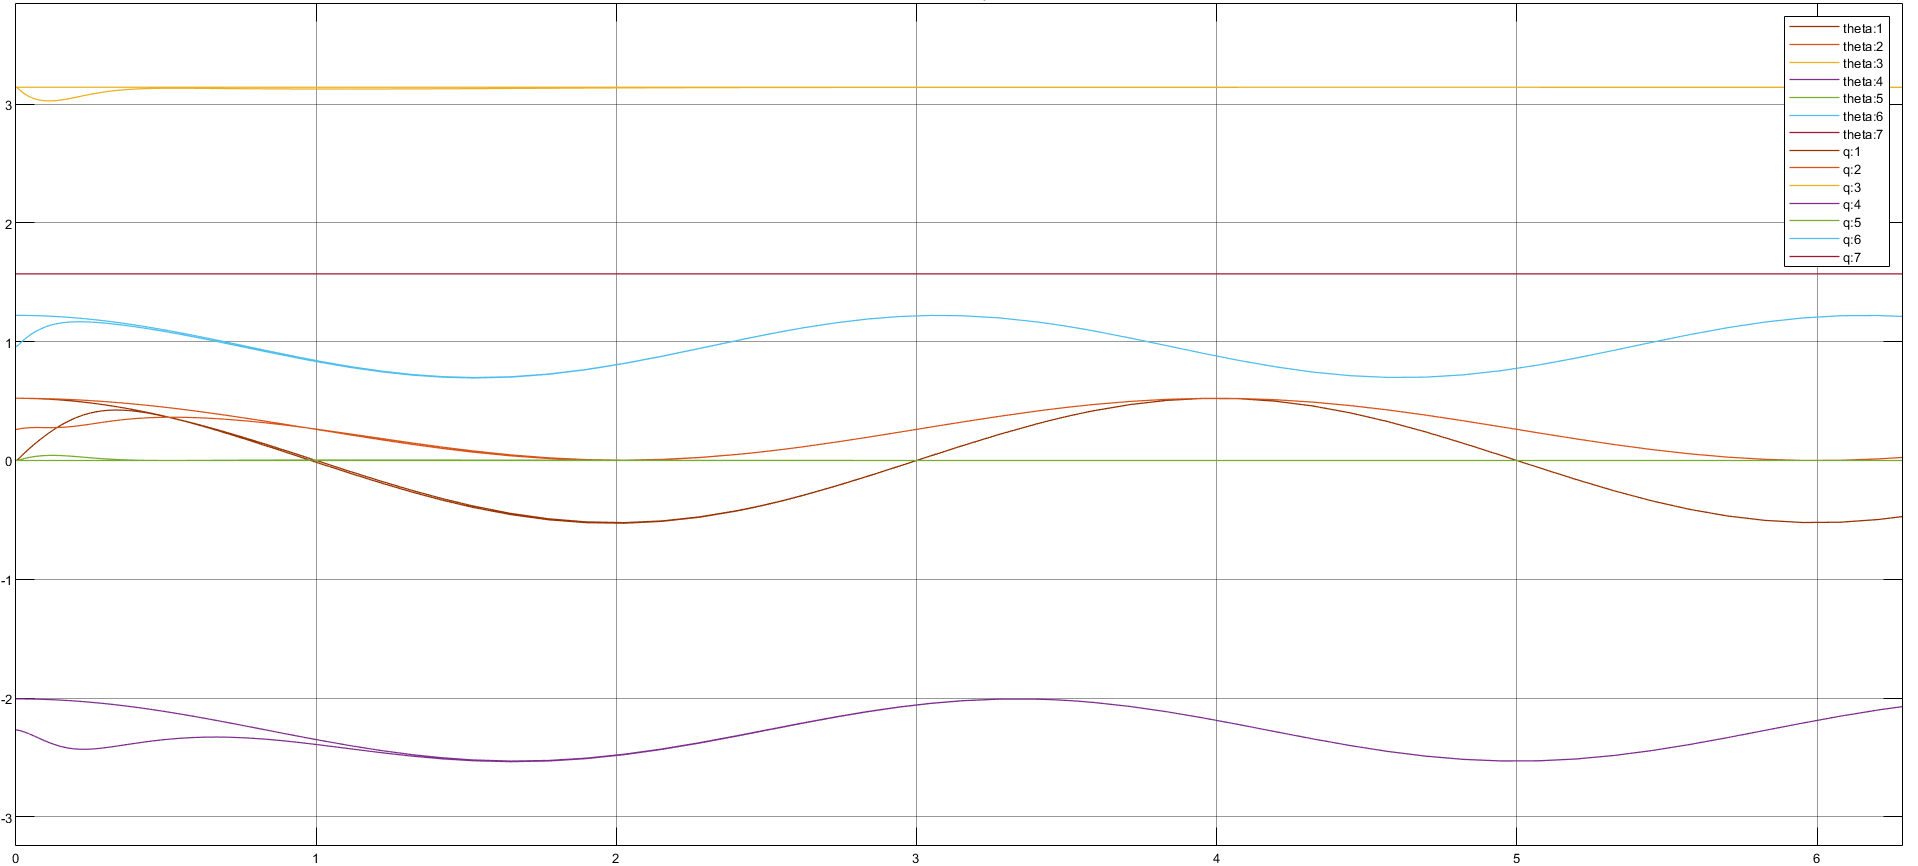
\includegraphics[width=\linewidth]{posicao_slotine_li_pi2.png}
        \caption{Posições das juntas}
        \label{fig:posicao_slotine_li_pi2}
    \end{subfigure}%
    \hfill
    \begin{subfigure}[b]{0.49\textwidth}
        \centering
        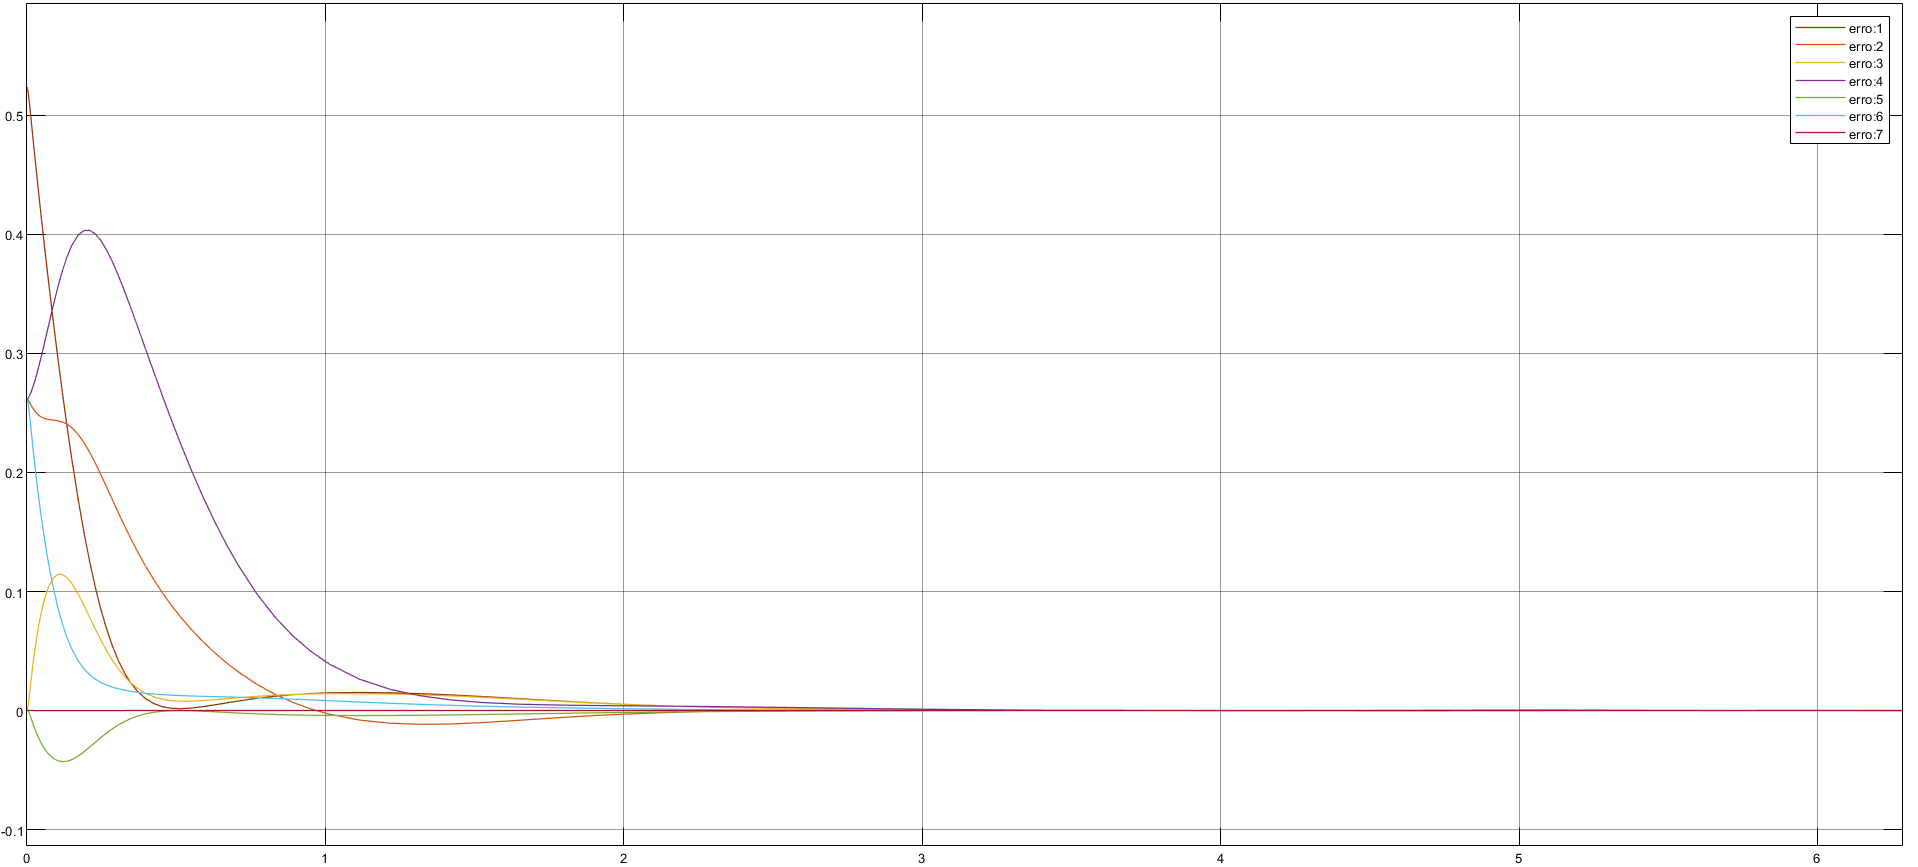
\includegraphics[width=\linewidth]{erro_slotine_li_pi2.png}
        \caption{Erros de posições das juntas}
        \label{fig:erro_slotine_li_pi2}
    \end{subfigure}%
    \hfill
    \begin{subfigure}[b]{0.49\textwidth}
        \centering
        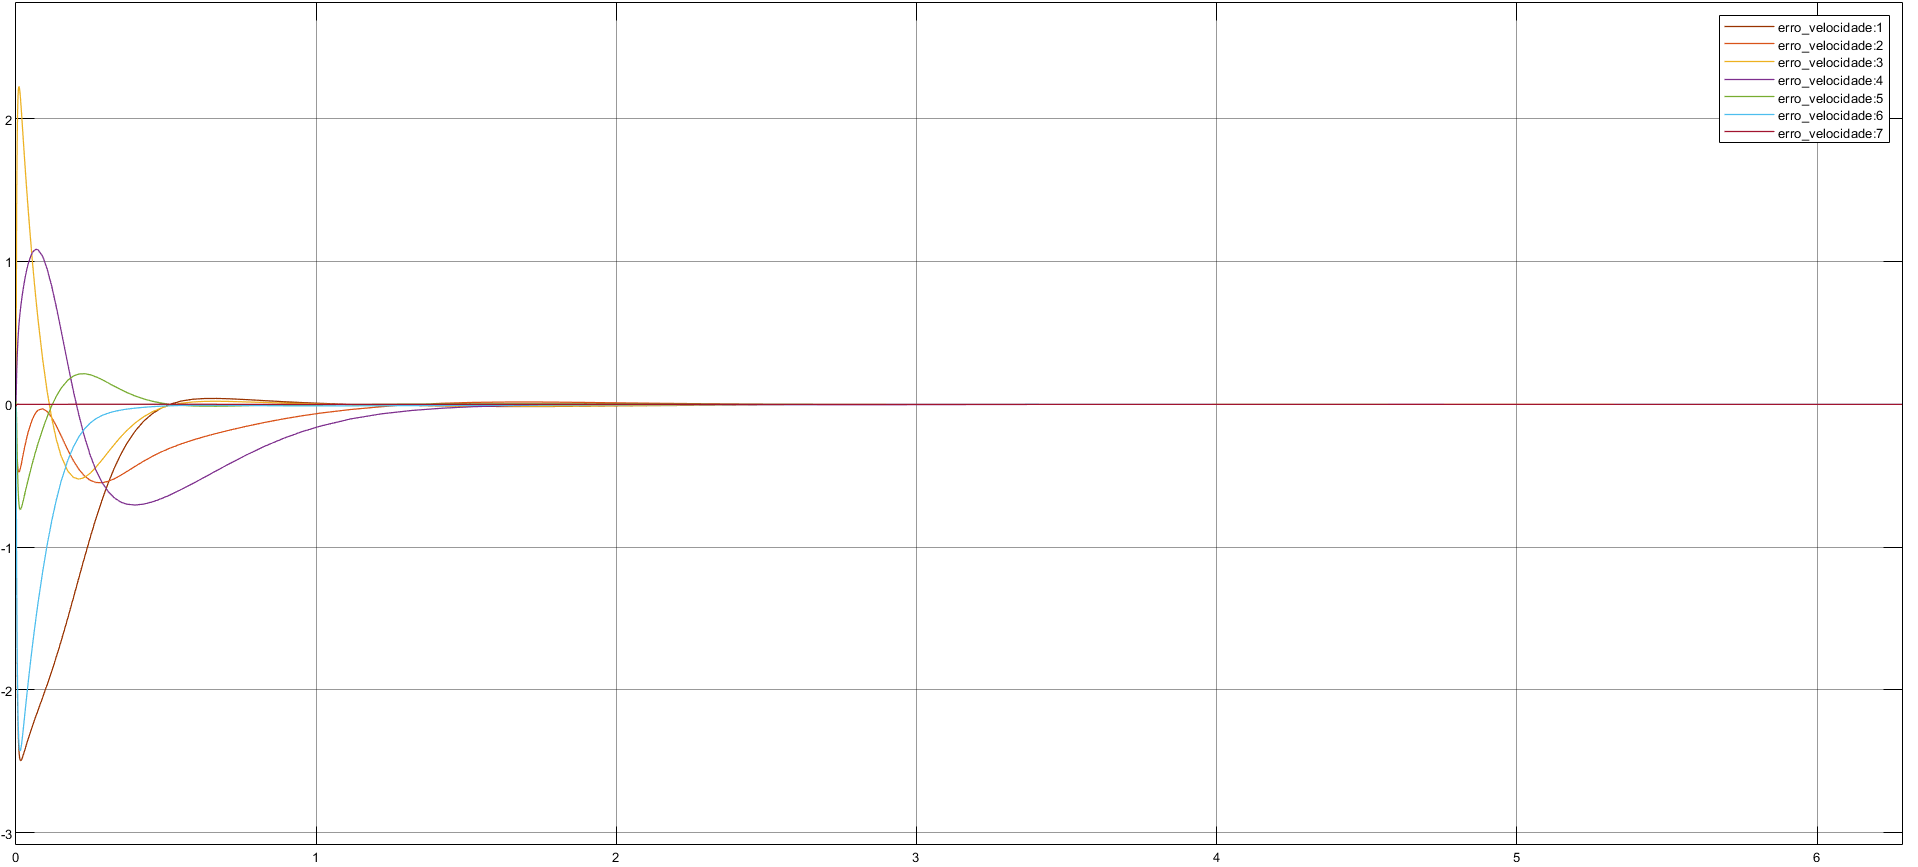
\includegraphics[width=\linewidth]{erro_velocidade_slotine_li_pi2.png}
        \caption{Erros de velocidades das juntas}
        \label{fig:erro_velocidade_slotine_li_pi2}
    \end{subfigure}%
    \caption{Controlador por Slotine \& Li ($\omega_n = \pi/2$)}
    \label{fig:imagens_slotine_li_pi2}
\end{figure}

Além disso, foi feito a simulação com a massa adicional de 10kg para $\omega_n = \pi$:

\begin{figure}[h!]
    \centering
    \begin{subfigure}[b]{0.47\textwidth}
        \centering
        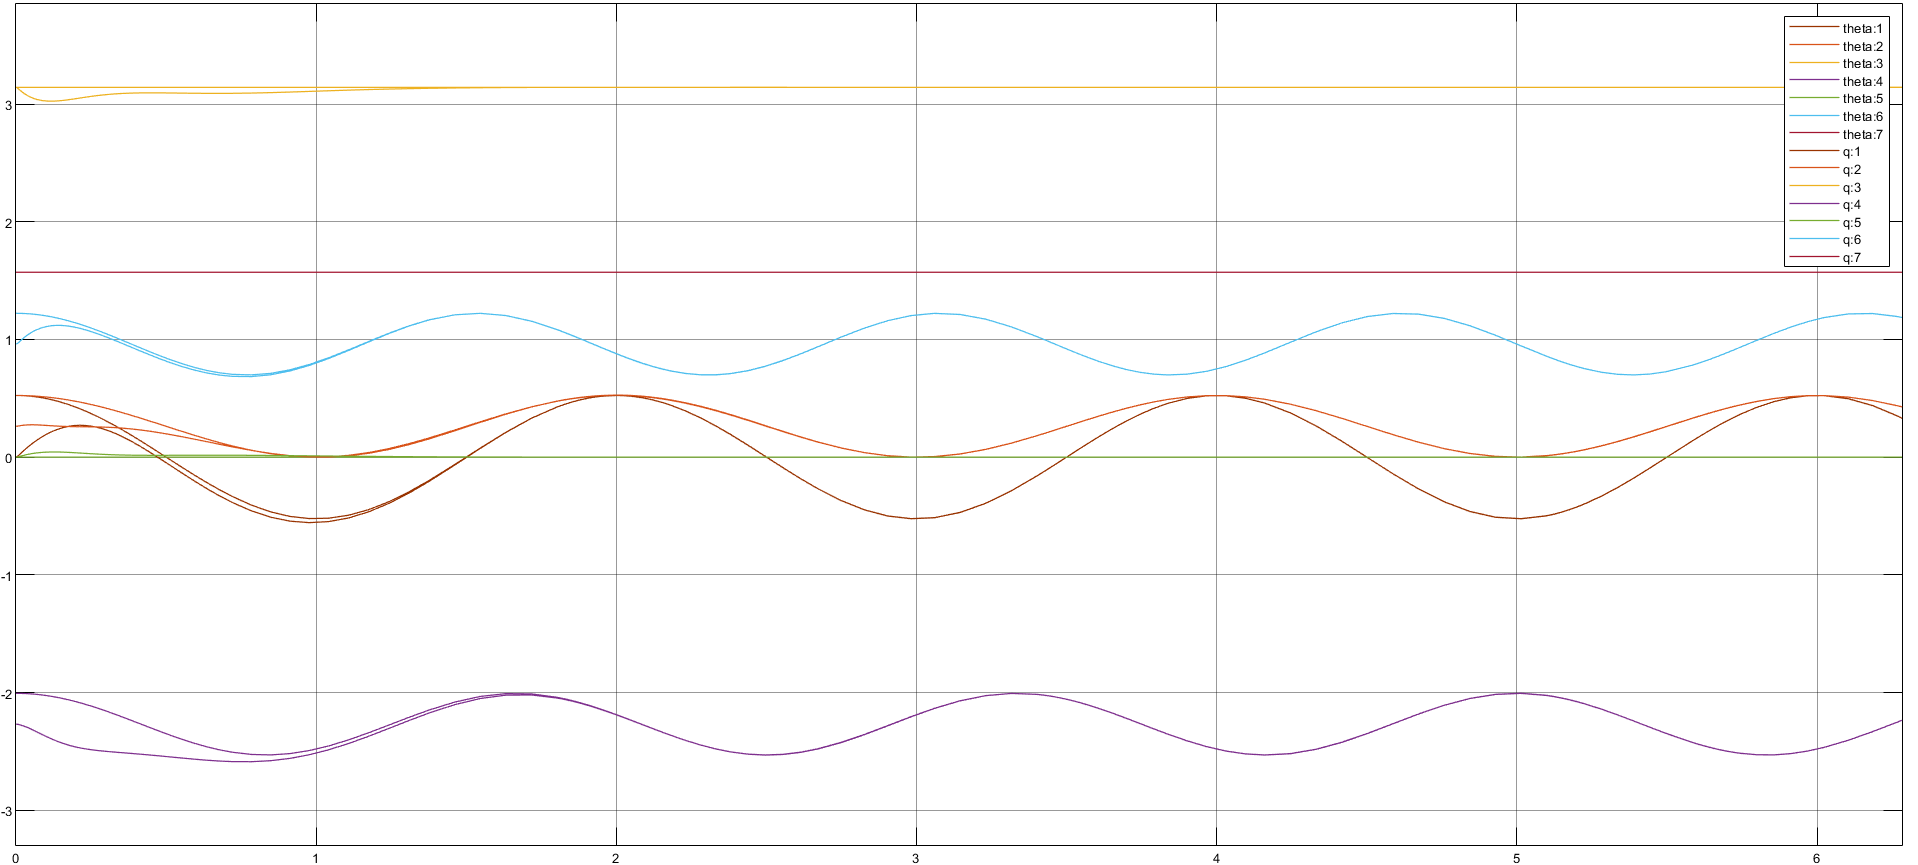
\includegraphics[width=\linewidth]{posicao_slotine_li_pi_m.png}
        \caption{Posições das juntas}
        \label{fig:posicao_slotine_li_pi_m}
    \end{subfigure}%
    \hfill
    \begin{subfigure}[b]{0.47\textwidth}
        \centering
        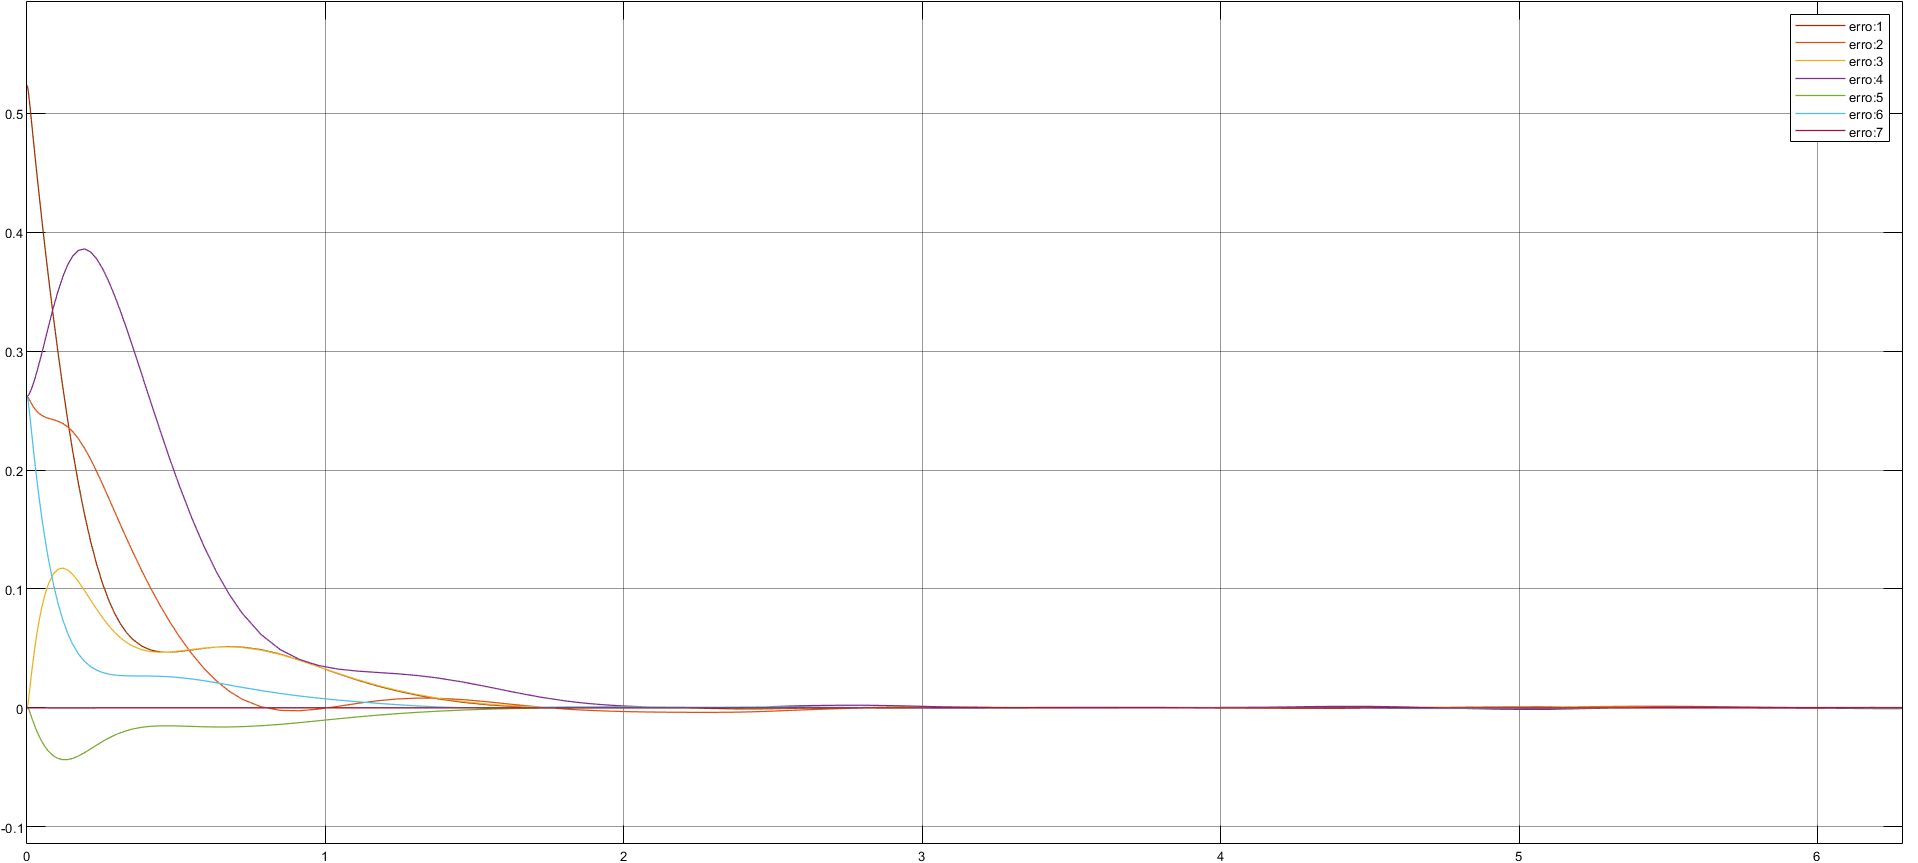
\includegraphics[width=\linewidth]{erro_slotine_li_pi_m.png}
        \caption{Erros de posições das juntas}
        \label{fig:erro_slotine_li_pi_m}
    \end{subfigure}%
    \hfill
    \begin{subfigure}[b]{0.47\textwidth}
        \centering
        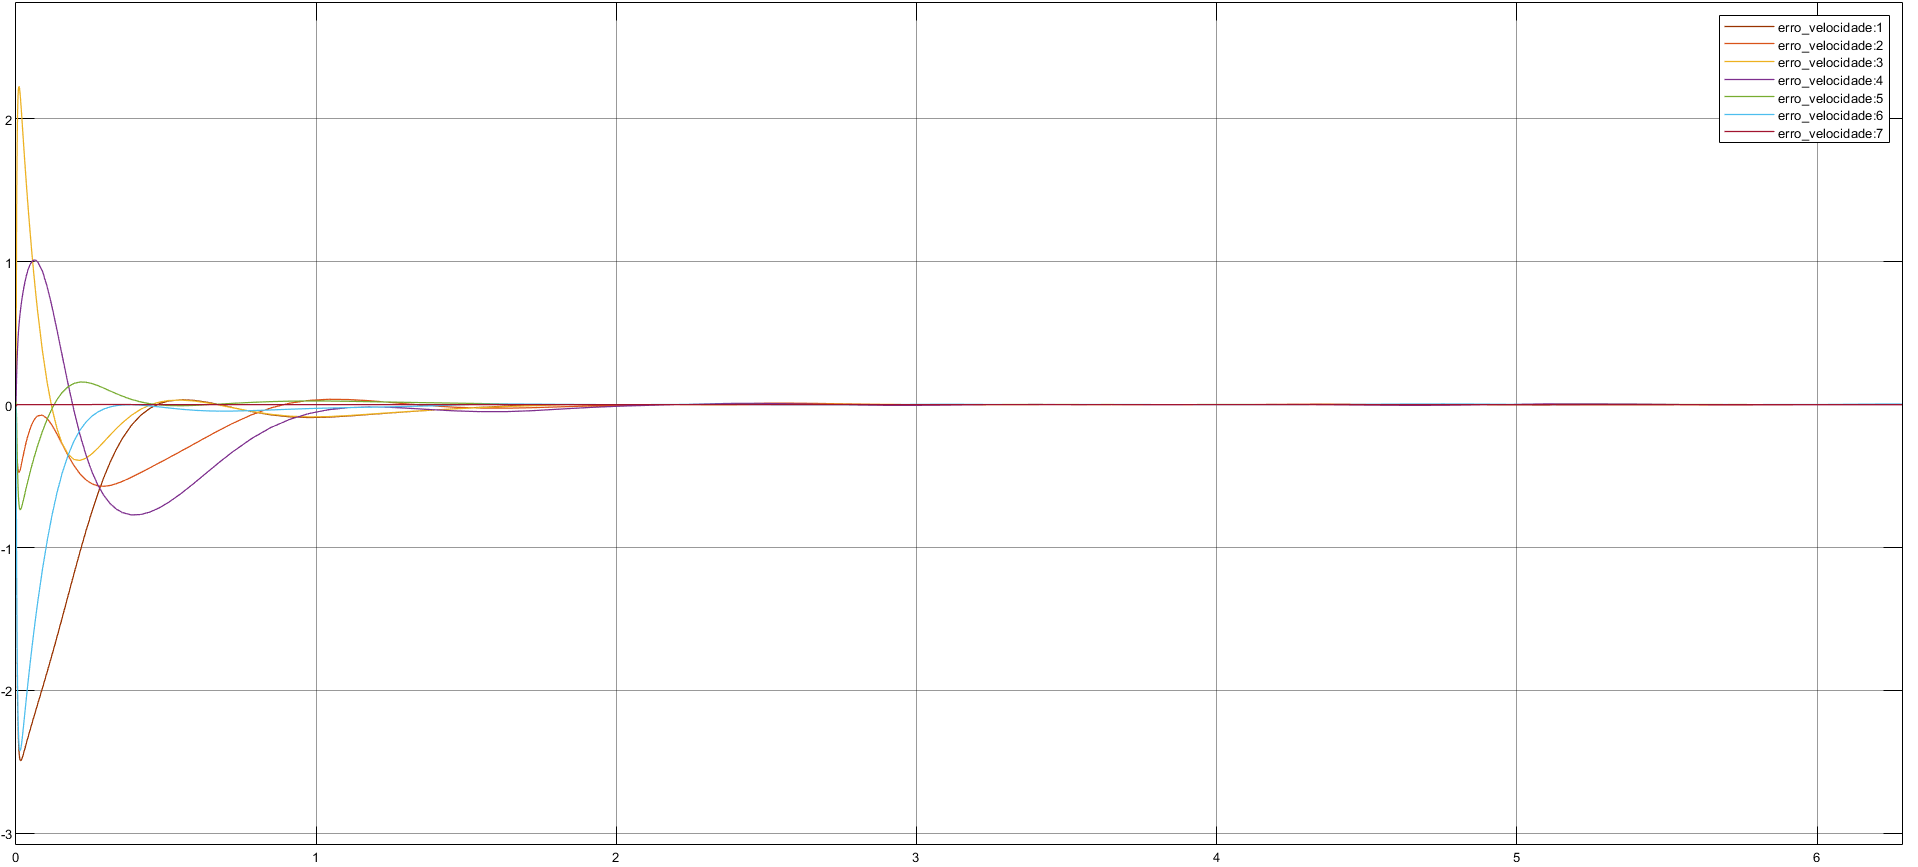
\includegraphics[width=\linewidth]{erro_velocidade_slotine_li_pi_m.png}
        \caption{Erros de velocidades das juntas}
        \label{fig:erro_velocidade_slotine_li_pi_m}
    \end{subfigure}%
    \caption{Controlador por Slotine \& Li ($\omega_n = \pi$)}
    \label{fig:imagens_slotine_li_pi_m}
\end{figure}

Ademais, foi feito a simulação com a massa adicional de 10kg para $\omega_n = \pi/2$:
\begin{figure}[h!]
    \centering
    \begin{subfigure}[b]{0.47\textwidth}
        \centering
        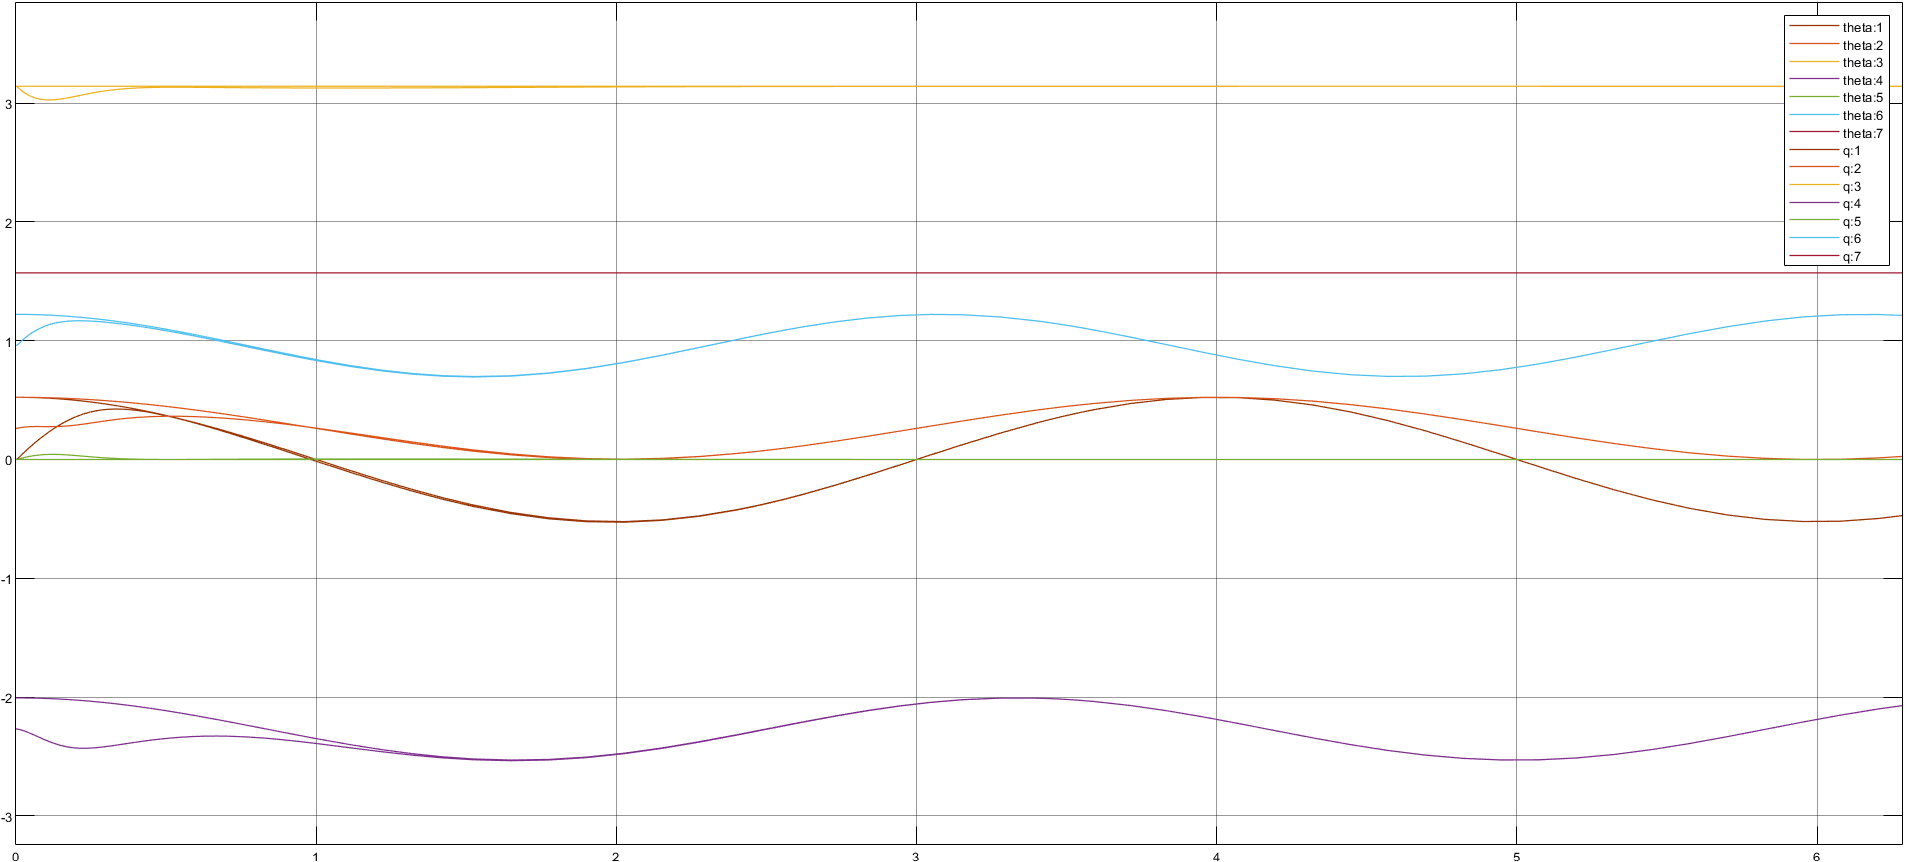
\includegraphics[width=\linewidth]{posicao_slotine_li_pi2_m.png}
        \caption{Posições das juntas}
        \label{fig:posicao_slotine_li_pi2_m}
    \end{subfigure}%
    \hfill
    \begin{subfigure}[b]{0.47\textwidth}
        \centering
        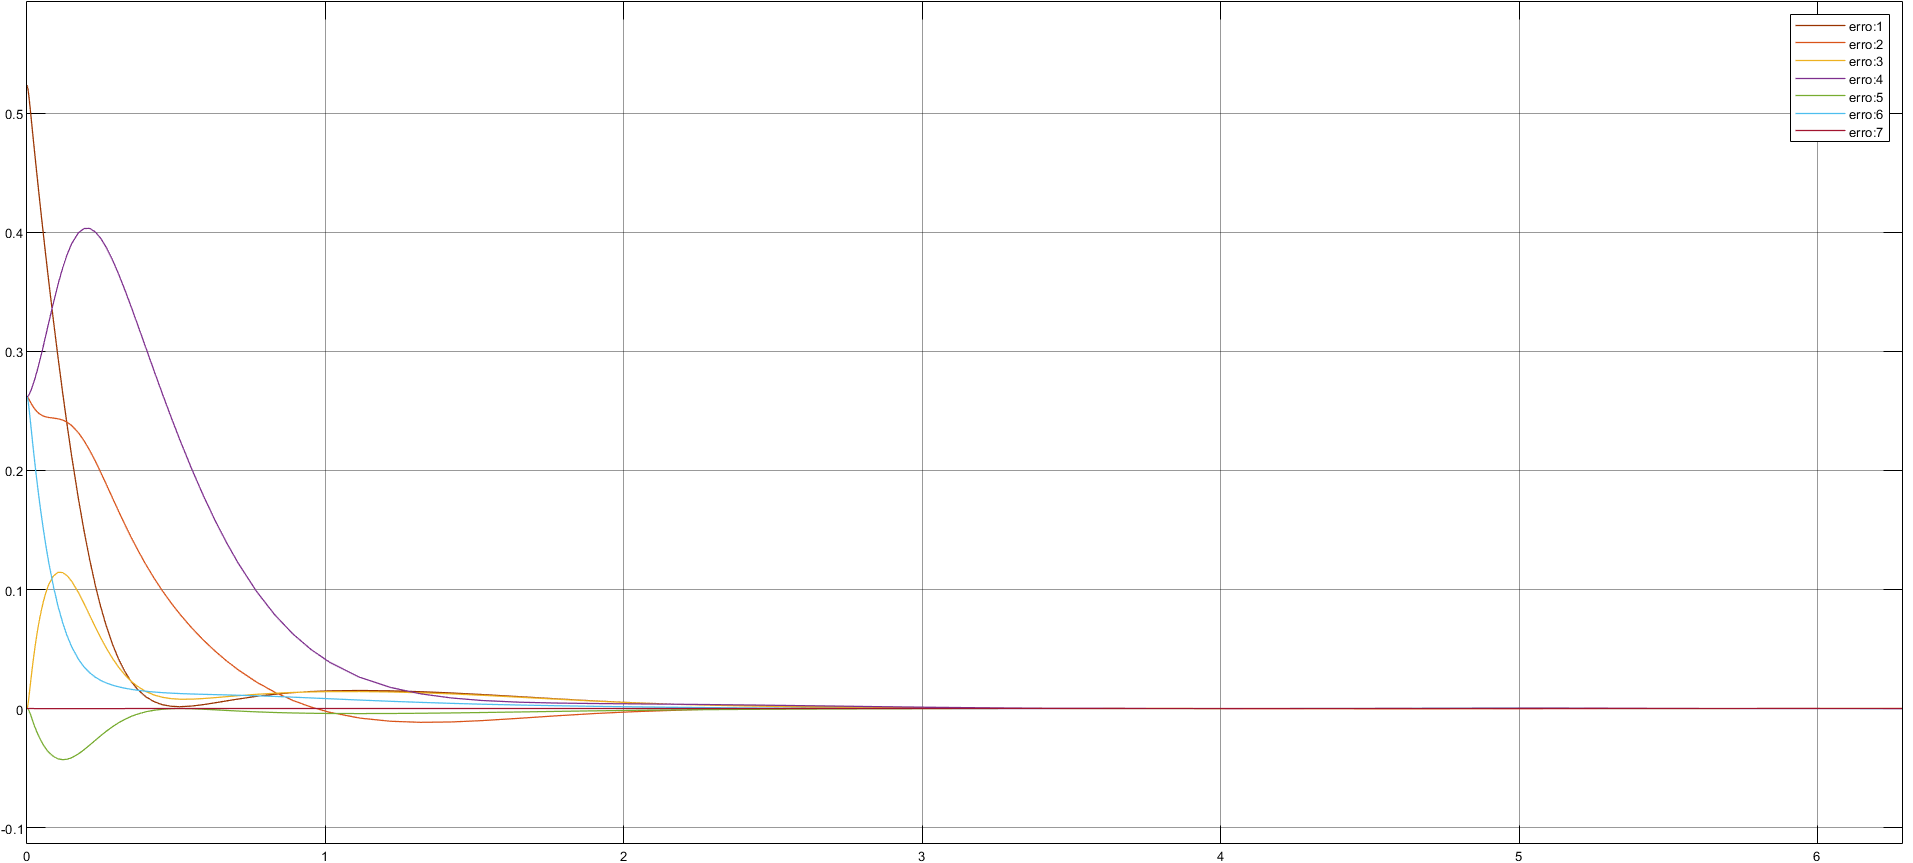
\includegraphics[width=\linewidth]{erro_slotine_li_pi2_m.png}
        \caption{Erros de posições das juntas}
        \label{fig:erro_slotine_li_pi2_m}
    \end{subfigure}%
    \hfill
    \begin{subfigure}[b]{0.47\textwidth}
        \centering
        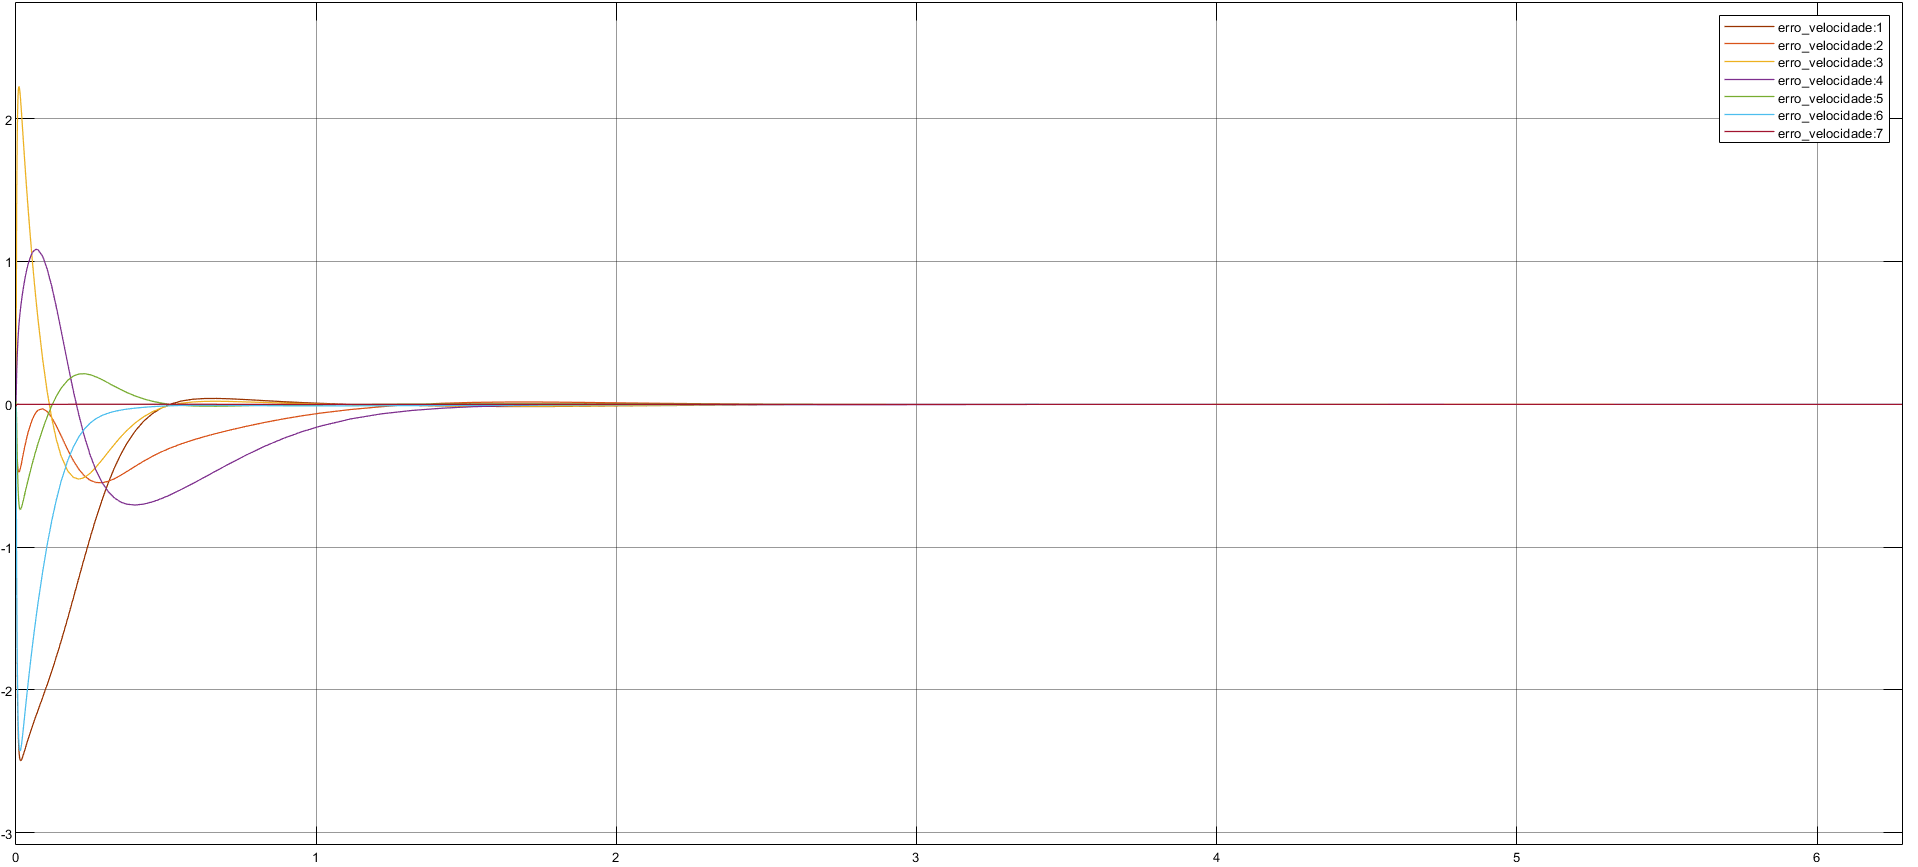
\includegraphics[width=\linewidth]{erro_velocidade_slotine_li_pi2_m.png}
        \caption{Erros de velocidades das juntas}
        \label{fig:erro_velocidade_slotine_li_pi2_m}
    \end{subfigure}%
    \caption{Controlador por Slotine \& Li ($\omega_n = \pi/2$)}
    \label{fig:imagens_slotine_li_pi2_m}
\end{figure}

\section{Conclusão}

Após a implementação e simulação dos controladores PD, P-PI, Torque Computado + PD e Slotine \& Li no manipulador Kinova Gen3, considerando trajetórias rápidas e lentas, e a alteração de massa do último elo, conclui-se que quase todos os controladores demonstraram desempenho estável e adequado em condições nominais, mas o controlador PD não teve um desempenho adequado por não conseguir seguir as trajetórias por não ter uma parcela integradora para zerar o erro em regime permanente e diferiram em robustez frente à alteração de massa. 

Ao adicionar uma massa de 10kg no último efetuador, os controladores PD e P-PI pioraram consideravelmente o resultado no quesito estabilidade, já o Torque Computado + PD conseguiu manter a estabilidade e o desempenho, enquanto o controlador de Slotine \& Li manteve a estabilidade, mas perdeu desempenho comparado com o projetado. 

Os controladores P-PI e por Torque Computado + PD apresentaram melhor desempenho em rastreamento de trajetórias, devido, respectivamente, à parcela integradora do controlador PI e à compensação explícita de termos dinâmicos, enquanto o controlador de Slotine \& Li destacou-se pela robustez em cenários de incerteza dinâmica. Por outro lado, o controlador PD apresentou oscilações e menor precisão nas condições modificadas.


\newpage

\section*{Apêndice}

\begin{lstlisting}[caption={Código principal do trabalho}, label={code:codigo}]
% Definindo a cinematica direta do Kinova Gen3 usando o padrao DH (Denavit-Hartenberg)
clear L
% Definicao dos parametros DH para cada elo do robo
%            theta    d(m)     a    alpha type offset
L(1) = Link([  0      -0.2848  0      pi/2  0   0], 'standard');
L(2) = Link([  0      -0.0118  0      pi/2  0   pi], 'standard');
L(3) = Link([  0      -0.4208  0      pi/2  0   pi], 'standard');
L(4) = Link([  0      -0.0128  0      pi/2  0   pi], 'standard');
L(5) = Link([  0      -0.3143  0      pi/2  0   pi], 'standard');
L(6) = Link([  0      0        0      pi/2  0   pi], 'standard');
L(7) = Link([  0      0        0      pi    0   pi], 'standard');

% Convertendo os frames do URDF para os frames do padrao DH
% Definicao das transformacoes homogeneas para alinhar os frames
% Frame 1
R1 = rotx(-90);
P1 = [0;0.12837;0];
T1 = SE3(R1, P1);

% Frame 2
R2 = rotx(-90)*rotz(180);
P2 = [0;0.006425; -0.00001];
T2 = SE3(R2, P2);

% Frame 3
R3 = rotx(-90);
P3 = [0;0.21041;0.00005];
T3 = SE3(R3, P3);

% Frame 4
R4 = roty(180)*rotx(-90);
P4 = [0;0.006475;0.00003];
T4 = SE3(R4, P4);

% Frame 5
R5 = rotx(-90);
P5 = [0;0.1059;0.0001];
T5 = SE3(R5, P5);

% Frame 6
R6 = roty(180)*rotx(-90);
P6 = [0;-0.00007505;-0.00003];
T6 = SE3(R6, P6);

% Frame 7
R7 = rotx(180);
P7 = [0;-0.0002501;0.10596];
T7 = SE3(R7, P7);

% Definicao dos parametros dinamicos do robo
% Massa, centro de massa e inercia para cada elo
L(1).m = 1.377; % Massa do shoulder_link
cmass1 = T1.T*[-2.3E-05; -0.010364; -0.07336; 1];
L(1).r = cmass1(1:3); % Centro de massa
L(1).I = [0.00457, 0.004831, 0.001409, 1E-06, 0.000448, 2E-06]; % Inercia

L(2).m = 1.163; % Massa do half_arm_1_link
cmass2 = T2.T*[-4.4E-05; -0.09958; -0.013278; 1];
L(2).r = cmass2(1:3);
L(2).I = [0.011088, 0.001072, 0.011255, 5E-06, -0.000691, 0];

L(3).m = 1.163; % Massa do half_arm_2_link
cmass3 = T3.T*[-4.4E-05; -0.006641; -0.117892; 1];
L(3).r = cmass3(1:3);
L(3).I = [0.010932, 0.011127, 0.001043, 0, 0.000606, -7E-06];

L(4).m = 0.93; % Massa do forearm_link
cmass4 = T4.T*[-1.8E-05; -0.075478; -0.015006; 1];
L(4).r = cmass4(1:3);
L(4).I = [0.008147, 0.000631, 0.008316, -1E-06, -0.0005, 0];

L(5).m = 0.678; % Massa do spherical_wrist_1_link
cmass5 = T5.T*[1E-06; -0.009432; -0.063883; 1];
L(5).r = cmass5(1:3);
L(5).I = [0.001596, 0.001607, 0.000399, 0, 0.000256, 0];

L(6).m = 0.678; % Massa do spherical_wrist_2_link
cmass6 = T6.T*[1E-06; -0.045483; -0.00965; 1];
L(6).r = cmass6(1:3);
L(6).I = [0.001641, 0.00041, 0.001641, 0, -2E-06, 0];

L(7).m = 0.364; % Massa do bracelet_link + end-effector
cmass7 = T7.T*[-9.3E-05; 0.000132; -0.022905; 1];
L(7).r = cmass7(1:3);
L(7).I = [0.000214, 0.000223, 0.00024, 0, -2E-06, 1E-06];

% Inicializar a inercia do motor para todas as juntas como zero
for i = 1:7
    L(i).Jm = 0;
end

% Criando o modelo dinamico do robo Kinova Gen3
kinova = SerialLink(L, 'name', 'Kinova Gen3');

% Definir a transformacao base do robo
Tb0 = trotx(180);
kinova.base = Tb0;

% Inicializar a matriz M_bar como uma matriz diagonal
M_bar = zeros(7, 7);

% Calcular a matriz de inercia diagonal M_bar
for i = 1:7
    % Inicializar o termo diagonal da junta i
    M_bar_i = 0;
    % Acumulador para a distancia ao longo das juntas
    distancia_acumulada = 0;
    for j = i:7
        % Adicionar o termo de inercia e centro de massa
        M_bar_i = M_bar_i + L(j).I(3,3) + L(j).m * (norm(L(j).r)^2 + (distancia_acumulada));

        % Distancia acumulada ate a junta atual
        distancia_acumulada = distancia_acumulada + abs(L(j).d)^2; % Somar comprimento da junta
    end
    % Preencher o elemento diagonal correspondente
    M_bar(i, i) = M_bar_i;
end

% Adicao de uma massa adicional de 10kg no "end effector link"
L_alterado = L;
L_alterado(7).m = 10.364;

% Calculo do centro de massa alterado
cmass_alterado = (0.364 * cmass7(1:3) + 10 * [0; 0; 0.1674]) / 10.364;
L_alterado(7).r = cmass_alterado;

% Inercia devido a massa adicional (em forma de vetor)
inercia_massa_adicional = (0.1674 - cmass_alterado(3))^2 * 10 * [1, 1, 0, 0, 0, 0];

% Inercia antiga no formato de matriz
inercia_antiga = [0.000214, 0.000223, 0.00024, 0, -2E-06, 1E-06];
I_A = [inercia_antiga(1), inercia_antiga(4), inercia_antiga(6); 
        inercia_antiga(4), inercia_antiga(2), inercia_antiga(5); 
        inercia_antiga(6), inercia_antiga(5), inercia_antiga(3)];

% Vetor de deslocamento entre os centros de massa antigo e alterado
d = cmass_alterado - cmass7(1:3);

% Matriz de inercia no novo ponto (teorema dos eixos paralelos)
I_P = I_A - 0.364 * ((d * d') - (d' * d) * eye(3) );

% Conversao da matriz de inercia alterada para o formato de vetor
inercia_massa_antiga_vec = [I_P(1,1), I_P(2,2), I_P(3,3), I_P(1,2), I_P(1,3), I_P(2,3)];

% Soma da nova inercia no formato de vetor
L_alterado(7).I = inercia_massa_adicional + inercia_massa_antiga_vec;

% Criando o modelo dinamico do robo Kinova Gen3
kinova_alterado = SerialLink(L_alterado, 'name', 'Kinova Gen3 Alterado');

% Definir a transformacao base do robo
kinova_alterado.base = Tb0;    
\end{lstlisting}

\end{document}